\documentclass[11pt]{article}
\usepackage{amsmath,amssymb,amsthm}
\usepackage[margin=1in]{geometry}
\usepackage[colorlinks=true,linkcolor=blue,urlcolor=blue]{hyperref}
\usepackage{multicol}
\usepackage{enumitem}
\usepackage{tikz}
\usetikzlibrary{calc,arrows.meta,decorations.pathreplacing}

\setlength{\parindent}{0pt}
\setlength{\parskip}{4pt}
\setcounter{secnumdepth}{0}  % unnumbered but TOC-linked sections

\newtheoremstyle{compact}{4pt}{2pt}{}{}{\bfseries}{.}{.5em}{}
\theoremstyle{compact}
\newtheorem{thm}{Theorem}[section]
\newtheorem{defn}[thm]{Definition}
\newtheorem{prop}[thm]{Property}

\renewcommand{\vec}[1]{\mathbf{#1}}
\newcommand{\vv}[1]{\langle #1 \rangle}
\newcommand{\ds}{\displaystyle}
\newcommand{\R}{\mathbb{R}}
\newcommand{\grad}{\nabla}
\newcommand{\ihat}{\hat{\mathbf{i}}}
\newcommand{\jhat}{\hat{\mathbf{j}}}
\newcommand{\khat}{\hat{\mathbf{k}}}

\begin{document}

\begin{center}
{\LARGE\bfseries Math 2531 Outline}\\[4pt]
{\large Multivariable Calculus . Stewart 9th ed.}
\end{center}

\tableofcontents
\newpage

%=======================================================================
\section{Definitions and Results . Quick Reference}
%=======================================================================

\subsection{Ch.\ 10: Parametric \& Polar}
\begin{enumerate}[label=\textbf{10.\arabic*.},leftmargin=*,itemsep=1pt]
  \item \textbf{Parametric curve}: $x=f(t)$, $y=g(t)$. Slope: $dy/dx=(dy/dt)/(dx/dt)$.
  \item \textbf{Horizontal tangent}: $dy/dt=0$, $dx/dt\ne0$. \textbf{Vertical tangent}: $dx/dt=0$, $dy/dt\ne0$.
  \item \textbf{Arc length} (parametric): $L=\int_\alpha^\beta\sqrt{(dx/dt)^2+(dy/dt)^2}\,dt$.
  \item \textbf{Area} (parametric, left-to-right): $A=\int_\alpha^\beta y\,(dx/dt)\,dt$.
  \item \textbf{Polar conversion}: $x=r\cos\theta$, $y=r\sin\theta$; $r^2=x^2+y^2$, $\tan\theta=y/x$.
  \item \textbf{Polar area}: $A=\tfrac{1}{2}\int_\alpha^\beta r^2\,d\theta$. Between curves: $A=\tfrac{1}{2}\int_\alpha^\beta(r_{\rm out}^2-r_{\rm in}^2)\,d\theta$.
  \item \textbf{Polar arc length}: $L=\int_\alpha^\beta\sqrt{r^2+(dr/d\theta)^2}\,d\theta$.
\end{enumerate}

\subsection{Ch.\ 12: Vectors \& Geometry of Space}
\begin{enumerate}[label=\textbf{12.\arabic*.},leftmargin=*,itemsep=1pt]
  \item \textbf{Distance}: $|P_1P_2|=\sqrt{(x_2-x_1)^2+(y_2-y_1)^2+(z_2-z_1)^2}$.
  \item \textbf{Sphere}: $(x-h)^2+(y-k)^2+(z-l)^2=r^2$.
  \item \textbf{Magnitude}: $|\vec{a}|=\sqrt{a_1^2+a_2^2+a_3^2}$. \textbf{Unit vector}: $\hat{\vec{a}}=\vec{a}/|\vec{a}|$.
  \item \textbf{Dot product}: $\vec{a}\cdot\vec{b}=a_1b_1+a_2b_2+a_3b_3=|\vec{a}||\vec{b}|\cos\theta$.
  \item $\vec{a}\perp\vec{b}\iff\vec{a}\cdot\vec{b}=0$.
  \item \textbf{Direction cosines}: $\cos\alpha=a_1/|\vec{a}|$, $\cos\beta=a_2/|\vec{a}|$, $\cos\gamma=a_3/|\vec{a}|$; sum of squares $=1$.
  \item \textbf{Scalar proj}: $\mathrm{comp}_{\vec{a}}\vec{b}=\vec{a}\cdot\vec{b}/|\vec{a}|$. \textbf{Vector proj}: $\mathrm{proj}_{\vec{a}}\vec{b}=(\vec{a}\cdot\vec{b}/|\vec{a}|^2)\vec{a}$.
  \item \textbf{Cross product}: $\vec{a}\times\vec{b}=\langle a_2b_3-a_3b_2,\,a_3b_1-a_1b_3,\,a_1b_2-a_2b_1\rangle$; $|\vec{a}\times\vec{b}|=|\vec{a}||\vec{b}|\sin\theta$.
  \item $\vec{a}\times\vec{b}\perp\vec{a}$ and $\vec{a}\times\vec{b}\perp\vec{b}$; $\vec{a}\parallel\vec{b}\iff\vec{a}\times\vec{b}=\vec{0}$; anticommutative.
  \item \textbf{Area parallelogram} $=|\vec{a}\times\vec{b}|$. \textbf{Volume parallelepiped} $=|\vec{a}\cdot(\vec{b}\times\vec{c})|$.
  \item \textbf{Line}: $\vec{r}=\vec{r}_0+t\vec{v}$; parametric $x=x_0+at$, $y=y_0+bt$, $z=z_0+ct$.
  \item \textbf{Plane} (normal $\vec{n}$): $\vec{n}\cdot(\vec{r}-\vec{r}_0)=0$, i.e.\ $a(x-x_0)+b(y-y_0)+c(z-z_0)=0$.
  \item \textbf{Distance, point $P$ to plane}: pick any $Q_0$ on the plane; $D=\bigl|\overrightarrow{Q_0P}\cdot\hat{\vec{n}}\bigr|=|ax_1+by_1+cz_1+d|/|\vec{n}|$.
  \item \textbf{Quadric surfaces}: ellipsoid, elliptic/hyperbolic paraboloid, cone, hyperboloid (1- and 2-sheet). Identify by traces.
\end{enumerate}

\subsection{Ch.\ 13: Vector Functions}
\begin{enumerate}[label=\textbf{13.\arabic*.},leftmargin=*,itemsep=1pt]
  \item \textbf{Derivative}: $\vec{r}'(t)=\langle f'(t),g'(t),h'(t)\rangle$ (component-wise).
  \item \textbf{Unit tangent}: $\vec{T}(t)=\vec{r}'(t)/|\vec{r}'(t)|$.
  \item \textbf{Thm}: $|\vec{r}(t)|=c\Rightarrow\vec{r}'(t)\perp\vec{r}(t)$.
  \item \textbf{Product rules}: $(\vec{u}\cdot\vec{v})'=\vec{u}'\cdot\vec{v}+\vec{u}\cdot\vec{v}'$; $(\vec{u}\times\vec{v})'=\vec{u}'\times\vec{v}+\vec{u}\times\vec{v}'$.
  \item \textbf{Arc length}: $L=\int_a^b|\vec{r}'(t)|\,dt$; arc length function $s(t)=\int_a^t|\vec{r}'(u)|\,du$.
  \item \textbf{Curvature}: $\kappa=|\vec{T}'|/|\vec{r}'|=|\vec{r}'\times\vec{r}''|/|\vec{r}'|^3$. For $y=f(x)$: $\kappa=|f''|/(1+f'^2)^{3/2}$.
  \item \textbf{Principal unit normal}: $\vec{N}=\vec{T}'/|\vec{T}'|$ (toward center of curvature). Radius of curvature $\rho=1/\kappa$.
  \item \textbf{Velocity/speed/acceleration}: $\vec{v}=\vec{r}'$, speed$=|\vec{v}|=ds/dt$, $\vec{a}=\vec{v}'$.
  \item \textbf{Acceleration decomposition}: $\vec{a}=a_T\vec{T}+a_N\vec{N}$; $a_T=\vec{r}'\cdot\vec{r}''/|\vec{r}'|$; $a_N=|\vec{r}'\times\vec{r}''|/|\vec{r}'|=\kappa v^2$.
\end{enumerate}

\subsection{Ch.\ 14: Partial Derivatives}
\begin{enumerate}[label=\textbf{14.\arabic*.},leftmargin=*,itemsep=1pt]
  \item \textbf{Level curves/surfaces}: $f(x,y)=k$; $f(x,y,z)=k$.
  \item \textbf{Limit}: same value along \emph{every} path. To show DNE: find two paths with different limits.
  \item \textbf{Continuity}: $\lim_{(x,y)\to(a,b)}f=f(a,b)$.
  \item \textbf{Partial derivative}: $f_x=\lim_{h\to0}[f(x+h,y)-f(x,y)]/h$ (hold $y$ fixed).
  \item \textbf{Clairaut's Thm}: $f_{xy}=f_{yx}$ when both continuous.
  \item \textbf{Tangent plane}: $z-z_0=f_x(x_0,y_0)(x-x_0)+f_y(x_0,y_0)(y-y_0)$.
  \item \textbf{Linearization}: $L(x,y)=f(a,b)+f_x(a,b)(x-a)+f_y(a,b)(y-b)$.
  \item \textbf{Differentiability thm}: $f_x$, $f_y$ continuous near $(a,b)\Rightarrow f$ differentiable at $(a,b)$.
  \item \textbf{Total differential}: $dz=(\partial z/\partial x)dx+(\partial z/\partial y)dy$.
  \item \textbf{Chain rule}: $dz/dt=(\partial z/\partial x)(dx/dt)+(\partial z/\partial y)(dy/dt)$.
  \item \textbf{Implicit}: $\partial z/\partial x=-F_x/F_z$ from $F(x,y,z)=0$.
  \item \textbf{Directional derivative}: $D_{\vec{u}}f=\nabla f\cdot\vec{u}$ ($\vec{u}$ unit). $\max D_{\vec{u}}f=|\nabla f|$.
  \item \textbf{Gradient}: $\nabla f=\langle f_x,f_y\rangle$; $\nabla f\perp$ level curves; points toward steepest ascent.
  \item \textbf{Tangent plane to} $F(x,y,z)=k$: $\nabla F(P_0)\cdot\langle x-x_0,y-y_0,z-z_0\rangle=0$.
  \item \textbf{Critical point}: $f_x=f_y=0$ or a partial DNE.
  \item \textbf{Second Derivatives Test}: $D=f_{xx}f_{yy}-f_{xy}^2$. $D>0,f_{xx}>0$: min; $D>0,f_{xx}<0$: max; $D<0$: saddle.
  \item \textbf{Extreme Value Thm}: continuous $f$ on closed bounded $D$ attains abs.\ max and min.
  \item \textbf{Lagrange multipliers}: at an extremum of $f$ subject to $g=k$, $\nabla f=\lambda\nabla g$.
\end{enumerate}

\subsection{Ch.\ 15: Multiple Integrals}
\begin{enumerate}[label=\textbf{15.\arabic*.},leftmargin=*,itemsep=1pt]
  \item \textbf{Fubini (rectangle)}: $\iint_R f\,dA=\int_a^b\int_c^d f\,dy\,dx=\int_c^d\int_a^b f\,dx\,dy$.
  \item \textbf{Type I/II}: $\iint_D f\,dA=\int_a^b\int_{g_1(x)}^{g_2(x)}f\,dy\,dx$ or $\int_c^d\int_{h_1(y)}^{h_2(y)}f\,dx\,dy$.
  \item \textbf{Polar}: $\iint_D f\,dA=\int_\alpha^\beta\int_{r_1}^{r_2}f(r\cos\theta,r\sin\theta)\,r\,dr\,d\theta$. \quad($dA=r\,dr\,d\theta$)
  \item \textbf{Mass/CoM}: $m=\iint\rho\,dA$; $\bar x=M_y/m$, $\bar y=M_x/m$; $M_y=\iint x\rho\,dA$, $M_x=\iint y\rho\,dA$.
  \item \textbf{Moments of inertia}: $I_x=\iint y^2\rho\,dA$, $I_y=\iint x^2\rho\,dA$.
  \item \textbf{Triple integral / Fubini}: any order; $\iiint_E dV=$ volume of $E$.
  \item \textbf{Cylindrical}: $dV=r\,dz\,dr\,d\theta$; $x=r\cos\theta$, $y=r\sin\theta$, $z=z$.
  \item \textbf{Spherical}: $dV=\rho^2\sin\phi\,d\rho\,d\theta\,d\phi$; $x=\rho\sin\phi\cos\theta$, $y=\rho\sin\phi\sin\theta$, $z=\rho\cos\phi$.
\end{enumerate}

\subsection{Ch.\ 16: Vector Calculus}
\begin{enumerate}[label=\textbf{16.\arabic*.},leftmargin=*,itemsep=1pt]
  \item \textbf{Conservative field}: $\vec{F}=\nabla f$ (potential $f$).
  \item \textbf{Line integral (scalar)}: $\int_C f\,ds=\int_a^b f(\vec{r}(t))|\vec{r}'(t)|\,dt$.
  \item \textbf{Work}: $\int_C\vec{F}\cdot d\vec{r}=\int_a^b\vec{F}(\vec{r}(t))\cdot\vec{r}'(t)\,dt=\int_C P\,dx+Q\,dy+R\,dz$.
  \item \textbf{FTLI}: $\vec{F}=\nabla f\Rightarrow\int_C\vec{F}\cdot d\vec{r}=f(\vec{r}(b))-f(\vec{r}(a))$ (path-independent).
  \item \textbf{Conservative test} ($\R^2$, simply-connected): $\partial P/\partial y=\partial Q/\partial x$.
  \item \textbf{Closed-curve criterion}: $\vec{F}$ conservative $\iff\oint_C\vec{F}\cdot d\vec{r}=0$ for all closed $C$.
  \item \textbf{Green's Thm}: $\oint_C P\,dx+Q\,dy=\iint_D(Q_x-P_y)\,dA$ ($C$ positively oriented).
  \item \textbf{Area via Green's}: $A=\tfrac{1}{2}\oint_C(x\,dy-y\,dx)$.
  \item \textbf{Curl}: $\nabla\times\vec{F}=\langle R_y-Q_z,\,P_z-R_x,\,Q_x-P_y\rangle$. Conservative $\Rightarrow\mathrm{curl}\,\vec{F}=\vec{0}$.
  \item \textbf{Divergence}: $\nabla\cdot\vec{F}=P_x+Q_y+R_z$. $\mathrm{div}(\mathrm{curl}\,\vec{F})=0$.
  \item \textbf{Green's (vector form)}: $\oint_C\vec{F}\cdot d\vec{r}=\iint_D(\mathrm{curl}\,\vec{F})\cdot\hat{\mathbf{k}}\,dA$.
\end{enumerate}

\newpage

%                       --
\section{Chapter 10 Review: Parametric Curves and Polar Coordinates}
%                       --

\begin{center}
\begin{tikzpicture}[>=Latex,scale=1.3]
  \draw[->,gray!60] (-0.3,0)--(4.0,0) node[right,font=\tiny]{$x$};
  \draw[->,gray!60] (0,-0.3)--(0,2.2) node[above,font=\tiny]{$y$};
  \draw[thick,blue,->,domain=0:3.1,samples=40] plot[smooth] ({0.4+\x*0.45},{0.9+0.7*sin(\x r)});
  \draw[thick,blue,->,domain=3.1:6.2,samples=40] plot[smooth] ({0.4+\x*0.45},{0.9+0.7*sin(\x r)});
  \foreach \tt/\lbl/\pos in {0.7/t_0/{below left},3.1/t_{\pi}/{above},5.5/t_2/{above right}} {
    \pgfmathsetmacro{\xx}{0.4+\tt*0.45}
    \pgfmathsetmacro{\yy}{0.9+0.7*sin(\tt r)}
    \filldraw[black] (\xx,\yy) circle (1.3pt) node[\pos,font=\small,inner sep=2pt]{$\lbl$};
  }
\end{tikzpicture}
\end{center}

\subsection{10.1 Parametric Curves}

\textbf{Parametric equations.} $x=f(t)$, $y=g(t)$. As $t$ varies you trace a \emph{parametric curve}.

\textbf{Eliminating the parameter.} solve one equation for $t$, substitute into the other. parametric form tracks direction and speed; Cartesian does not.

\textbf{Circle} of radius $r$ centered at $(h,k)$:
\[
x = h + r\cos t,\quad y = k + r\sin t, \quad 0\le t\le 2\pi
\]

\textbf{Line segment} from $(x_0,y_0)$ to $(x_1,y_1)$:
\[
x = x_0+(x_1-x_0)t,\quad y = y_0+(y_1-y_0)t,\quad 0\le t\le 1
\]

\textbf{Direction.} an arrowhead on a parametric curve shows which way $t$ goes.

\begin{center}
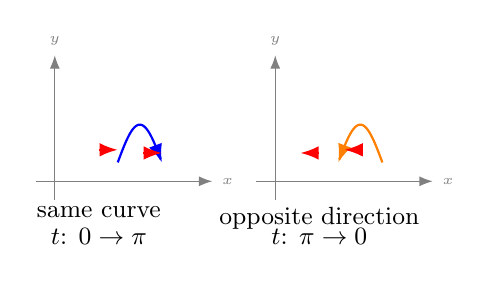
\begin{tikzpicture}[>=Latex,scale=0.8]
  \begin{scope}
    \draw[->,gray] (-0.3,0)--(2.5,0) node[right,font=\tiny]{$x$};
    \draw[->,gray] (0,-0.3)--(0,2.0) node[above,font=\tiny]{$y$};
    \draw[thick,blue,->,domain=0:3.14159,samples=40] plot ({1+0.7*\x/3.14159},{0.3+0.6*sin(\x r)});
    \draw[->,thick,red,shift={(0.7,0.5)}] (0,0)--(0.3,0);
    \draw[->,thick,red,shift={(1.4,0.45)}] (0,0)--(0.3,0);
    \node[below,font=\small] at (0.7,-0.25){same curve};
    \node[below,font=\small] at (0.7,-0.6){$t$: $0\to\pi$};
  \end{scope}
  \begin{scope}[xshift=3.5cm]
    \draw[->,gray] (-0.3,0)--(2.5,0) node[right,font=\tiny]{$x$};
    \draw[->,gray] (0,-0.3)--(0,2.0) node[above,font=\tiny]{$y$};
    \draw[thick,orange,->,domain=0:3.14159,samples=40] plot ({1.7-0.7*\x/3.14159},{0.3+0.6*sin(\x r)});
    \draw[->,thick,red,shift={(1.4,0.5)}] (0,0)--(-0.3,0);
    \draw[->,thick,red,shift={(0.7,0.45)}] (0,0)--(-0.3,0);
    \node[below,font=\small] at (0.7,-0.25){opposite direction};
    \node[below,font=\small] at (0.7,-0.6){$t$: $\pi\to 0$};
  \end{scope}
\end{tikzpicture}
\end{center}

\subsection{10.2 Calculus with Parametric Curves}

\textbf{Slope (tangent line).}
\[
\frac{dy}{dx} = \frac{dy/dt}{dx/dt}, \qquad \frac{dx}{dt}\ne 0
\]

\textbf{Horizontal tangent.} $dy/dt=0$ and $dx/dt\ne 0$.
\textbf{Vertical tangent.} $dx/dt=0$ and $dy/dt\ne 0$.

\textbf{Second derivative.}
\[
\frac{d^2y}{dx^2} = \frac{\dfrac{d}{dt}\!\left(\dfrac{dy}{dx}\right)}{dx/dt}
\]

\textbf{Arc length} ($f'$, $g'$ continuous, curve traced once):
\[
L = \int_\alpha^\beta \sqrt{\left(\frac{dx}{dt}\right)^2+\left(\frac{dy}{dt}\right)^2}\,dt
\]

\textit{Derivation.} pythagoras on the infinitesimal step gives $ds^2=dx^2+dy^2=\left(\frac{dx}{dt}\right)^2dt^2+\left(\frac{dy}{dt}\right)^2dt^2$ so $ds=\sqrt{(dx/dt)^2+(dy/dt)^2}\,dt$.

\textbf{Area under a parametric curve} (curve traversed left to right):
\[
A = \int_\alpha^\beta y\,\frac{dx}{dt}\,dt
\]

\begin{center}
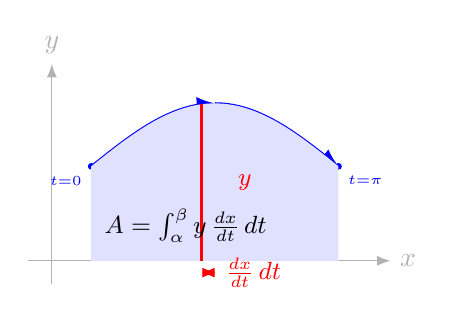
\begin{tikzpicture}[>=Latex,scale=1.0]
  \draw[->,gray!60] (-0.3,0)--(4.3,0) node[right]{$x$};
  \draw[->,gray!60] (0,-0.3)--(0,2.5) node[above]{$y$};
  % Parametric curve traced left to right
  \draw[blue,thick,->,domain=0:1.57,samples=30,variable=\t]
    plot ({0.5+\t},{1.2+0.8*sin(\t r)});
  \draw[blue,thick,->,domain=1.57:3.14,samples=30,variable=\t]
    plot ({0.5+\t},{1.2+0.8*sin(\t r)});
  \filldraw[blue] (0.5,1.2) circle (1pt) node[below left,font=\tiny]{$t{=}0$};
  \filldraw[blue] (3.64,1.2) circle (1pt) node[below right,font=\tiny]{$t{=}\pi$};
  \fill[blue!12]
    plot[domain=0:3.14,samples=60,variable=\t] ({0.5+\t},{1.2+0.8*sin(\t r)})
    -- (3.64,0) -- (0.5,0) -- cycle;
  % Sample slab of width dx at sample point
  \pgfmathsetmacro{\ts}{1.4}
  \pgfmathsetmacro{\xs}{0.5+\ts}
  \pgfmathsetmacro{\ys}{1.2+0.8*sin(\ts r)}
  \draw[red,thick] (\xs,0) -- (\xs,\ys);
  \draw[red,<->] (\xs,-0.15) -- (\xs+0.18,-0.15) node[right,red,font=\small]{$\tfrac{dx}{dt}\,dt$};
  \node[red,font=\small] at (\xs+0.55,{\ys/2}){$y$};
  \node[font=\small] at (1.7,0.45){$A=\int_\alpha^\beta y\,\tfrac{dx}{dt}\,dt$};
\end{tikzpicture}
\end{center}

\subsection{10.3 Polar Coordinates}

\textbf{Polar coordinates.} point $P$ is $(r,\theta)$ where $r=|OP|$ and $\theta$ is the angle from the polar axis. negative $r$ allowed: $(-r,\theta)=(r,\theta+\pi)$.

\begin{center}
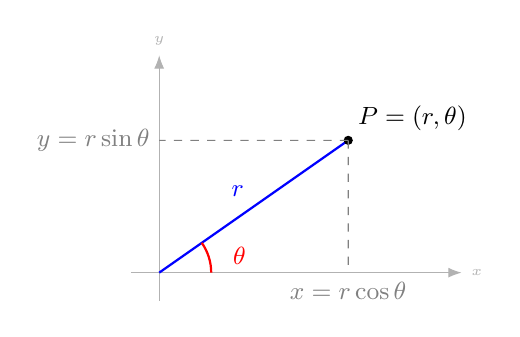
\begin{tikzpicture}[>=Latex,scale=1.2]
  \draw[->,gray!60] (-0.3,0)--(3.2,0) node[right,font=\tiny]{$x$};
  \draw[->,gray!60] (0,-0.3)--(0,2.3) node[above,font=\tiny]{$y$};
  \coordinate (P) at (2.0,1.4);
  \draw[thick,blue] (0,0) -- (P);
  \draw[red,thick] (0.55,0) arc (0:35:0.55);
  \node[red] at (0.85,0.18){\small$\theta$};
  \node[blue,above left] at (1.0,0.7){\small$r$};
  \filldraw (P) circle (1.2pt) node[above right]{\small$P=(r,\theta)$};
  \draw[dashed,gray] (P) -- (2.0,0) node[below]{\small$x=r\cos\theta$};
  \draw[dashed,gray] (P) -- (0,1.4) node[left]{\small$y=r\sin\theta$};
\end{tikzpicture}
\end{center}

\textbf{Conversion formulas.}
\[
x = r\cos\theta,\quad y = r\sin\theta \qquad\qquad r^2=x^2+y^2,\quad \tan\theta = \frac{y}{x}
\]

\textbf{Common curves} ($r$ at each angle $\theta$):

\begin{center}
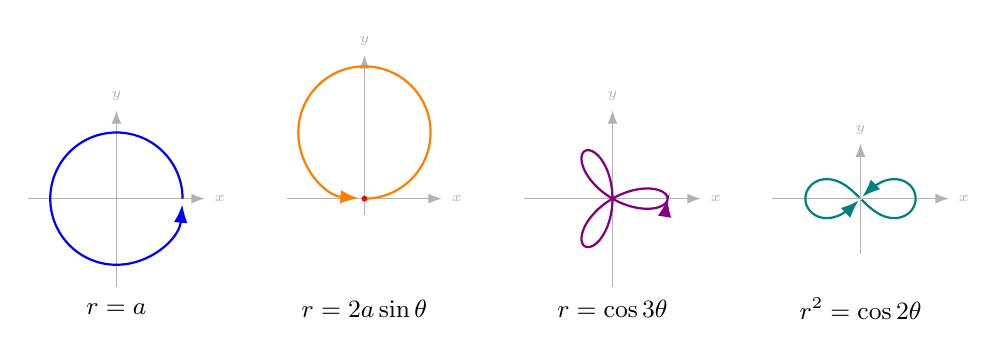
\begin{tikzpicture}[>=Latex,scale=0.7]
  % r = a (circle at origin)
  \begin{scope}
    \draw[->,gray!60] (-1.6,0)--(1.6,0) node[right,font=\tiny]{$x$};
    \draw[->,gray!60] (0,-1.6)--(0,1.6) node[above,font=\tiny]{$y$};
    \draw[thick,blue,->] (1.2,0) arc (0:355:1.2);
    \node at (0,-2){\small $r=a$};
  \end{scope}
  % r = 2a sin theta (circle through origin)
  \begin{scope}[xshift=4.5cm]
    \draw[->,gray!60] (-1.4,0)--(1.4,0) node[right,font=\tiny]{$x$};
    \draw[->,gray!60] (0,-0.3)--(0,2.6) node[above,font=\tiny]{$y$};
    \draw[thick,orange,->] (0,0) arc (-90:265:1.2);
    \filldraw[red] (0,0) circle (1.2pt);
    \node at (0,-2){\small $r=2a\sin\theta$};
  \end{scope}
  % rose r = cos(3 theta)
  \begin{scope}[xshift=9cm]
    \draw[->,gray!60] (-1.6,0)--(1.6,0) node[right,font=\tiny]{$x$};
    \draw[->,gray!60] (0,-1.6)--(0,1.6) node[above,font=\tiny]{$y$};
    \draw[thick,violet,->,domain=0:6.2832,samples=200] plot ({cos(3*\x r)*cos(\x r)},{cos(3*\x r)*sin(\x r)});
    \node at (0,-2){\small $r=\cos 3\theta$};
  \end{scope}
  % lemniscate r^2 = cos 2 theta
  \begin{scope}[xshift=13.5cm]
    \draw[->,gray!60] (-1.6,0)--(1.6,0) node[right,font=\tiny]{$x$};
    \draw[->,gray!60] (0,-1)--(0,1) node[above,font=\tiny]{$y$};
    \draw[thick,teal,->,domain=-0.785:0.785,samples=80] plot ({sqrt(cos(2*\x r))*cos(\x r)},{sqrt(cos(2*\x r))*sin(\x r)});
    \draw[thick,teal,->,domain=-0.785:0.785,samples=80] plot ({-sqrt(cos(2*\x r))*cos(\x r)},{-sqrt(cos(2*\x r))*sin(\x r)});
    \node at (0,-2){\small $r^2=\cos 2\theta$};
  \end{scope}
\end{tikzpicture}
\end{center}

\begin{center}
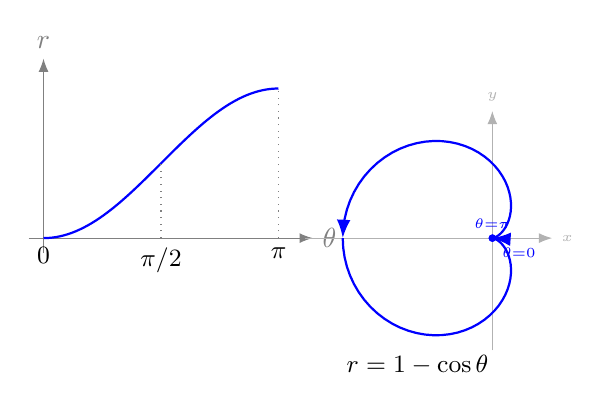
\begin{tikzpicture}[>=Latex,scale=0.95]
  % left: r vs theta plot
  \begin{scope}[xshift=-3.8cm]
    \draw[->,gray] (-0.2,0)--(3.6,0) node[right]{$\theta$};
    \draw[->,gray] (0,-0.2)--(0,2.4) node[above]{$r$};
    \draw[thick,blue,domain=0:3.14159,samples=60] plot (\x,{1-cos(\x r)});
    \foreach \t in {0,1.5708,3.14159} \draw[gray,dotted] (\t,0)--(\t,{1-cos(\t r)});
    \node[below] at (0,0){\small$0$};
    \node[below] at (1.5708,0){\small$\pi/2$};
    \node[below] at (3.14159,0){\small$\pi$};
  \end{scope}
  % right: polar curve
  \begin{scope}[xshift=2.2cm]
    \draw[->,gray!60] (-2.5,0)--(0.8,0) node[right,font=\tiny]{$x$};
    \draw[->,gray!60] (0,-1.5)--(0,1.7) node[above,font=\tiny]{$y$};
    \draw[thick,blue,->,domain=0:3.1416,samples=50] plot ({(1-cos(\x r))*cos(\x r)},{(1-cos(\x r))*sin(\x r)});
    \draw[thick,blue,->,domain=3.1416:6.2832,samples=50] plot ({(1-cos(\x r))*cos(\x r)},{(1-cos(\x r))*sin(\x r)});
    \filldraw (0,0) circle (0.8pt);
    \filldraw[blue] ({(1-cos(0))*cos(0)},{(1-cos(0))*sin(0)}) circle (1.2pt) node[below right,font=\tiny]{$\theta{=}0$};
    \filldraw[blue] ({(1-cos(3.1416))*cos(3.1416)},{(1-cos(3.1416))*sin(3.1416)}) circle (1.2pt) node[above,font=\tiny]{$\theta{=}\pi$};
    \node at (-1,-1.7){\small $r=1-\cos\theta$};
  \end{scope}
\end{tikzpicture}
\end{center}

\subsection{10.4 Calculus in Polar Coordinates}

\textbf{Tangent line} to $r=f(\theta)$: treat as parametric in $\theta$:
\[
\frac{dy}{dx} = \frac{(dr/d\theta)\sin\theta + r\cos\theta}{(dr/d\theta)\cos\theta - r\sin\theta}
\]

\textit{derivation.} from $x=r\cos\theta,\;y=r\sin\theta$, differentiate w.r.t.\ $\theta$ then divide.

\textbf{Area} swept by $r=f(\theta)$ from $\theta=\alpha$ to $\theta=\beta$:
\[
A = \frac{1}{2}\int_\alpha^\beta r^2\,d\theta
\]

\begin{center}
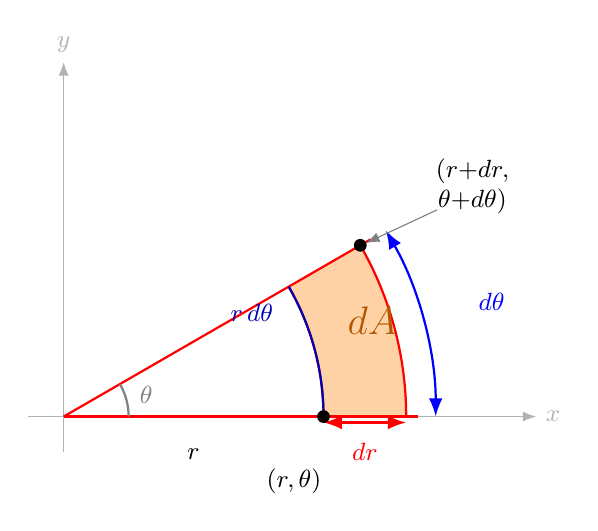
\begin{tikzpicture}[>=Latex,scale=1.5]
  \draw[->,gray!60] (-0.3,0)--(4.0,0) node[right,font=\small]{$x$};
  \draw[->,gray!60] (0,-0.3)--(0,3.0) node[above,font=\small]{$y$};
  % open the wedge wider: angles 8 to 30 deg, radii 2.2 to 2.9
  \pgfmathsetmacro{\ri}{2.2}\pgfmathsetmacro{\ro}{2.9}
  \fill[orange!35] (\ri,0) arc (0:30:\ri) -- ({\ro*cos(30)},{\ro*sin(30)}) arc (30:0:\ro) -- cycle;
  \draw[red,thick] (0,0) -- ({\ro*cos(0)+0.1},0);
  \draw[red,thick] (0,0) -- ({\ro*cos(30)+0.1*cos(30)},{\ro*sin(30)+0.1*sin(30)});
  \draw[red,thick] (\ri,0) arc (0:30:\ri);
  \draw[red,thick] (\ro,0) arc (0:30:\ro);
  % theta arc at origin
  \draw[gray,thick] (0.55,0) arc (0:30:0.55);
  \node[gray,font=\small] at (0.7,0.18){$\theta$};
  % d theta as the angle width, label moved well outside the upper-right arc
  \draw[blue,thick,<->] ({(\ro+0.25)*cos(0)},{(\ro+0.25)*sin(0)}) arc (0:30:{\ro+0.25});
  \node[blue,font=\small] at ({(\ro+0.85)*cos(15)},{(\ro+0.85)*sin(15)}){$d\theta$};
  % dr radial gap as a small double-arrow along the lower edge
  \draw[red,<->,thick] (\ri,-0.05)--(\ro,-0.05);
  \node[red,font=\small] at ({(\ri+\ro)/2},-0.3){$dr$};
  % arc r d theta drawn along the inner arc, label OUTSIDE on the upper side
  \draw[blue!70!black,thick] ({\ri*cos(0)},0) arc (0:30:\ri);
  \node[blue!70!black,font=\small] at ({(\ri-0.55)*cos(15)},{(\ri-0.55)*sin(15)+0.45}){$r\,d\theta$};
  % dA inside the wedge, well clear of the d theta label on the right
  \node[orange!70!black,font=\Large] at ({(\ri+\ro)/2*cos(15)+0.15},{(\ri+\ro)/2*sin(15)+0.15}){$dA$};
  % radial labels along the bottom only on the inner edge
  \node[font=\small] at ({\ri/2},-0.32){$r$};
  % Corner points - inner corner labelled to the left below the x axis, outer top-right with leader
  \filldraw[black] (\ri,0) circle (1.4pt);
  \node[font=\small] at (\ri-0.25,-0.55){$(r,\theta)$};
  \filldraw[black] ({\ro*cos(30)},{\ro*sin(30)}) circle (1.4pt);
  \node[font=\small,align=center] at ({\ro*cos(30)+0.95},{\ro*sin(30)+0.5}){$(r{+}dr,$\\ $\theta{+}d\theta)$};
  \draw[gray,thin,->] ({\ro*cos(30)+0.65},{\ro*sin(30)+0.3})--({\ro*cos(30)+0.05},{\ro*sin(30)+0.02});
\end{tikzpicture}
\end{center}

\textit{thin sector of angle $d\theta$ and radius $r$ has area $\tfrac12 r^2\,d\theta$, from the wedge formula $A=\tfrac12 r^2\theta$.}

\textbf{Area between two polar curves} ($f(\theta)\ge g(\theta)\ge 0$):
\[
A = \frac{1}{2}\int_\alpha^\beta \bigl([f(\theta)]^2 - [g(\theta)]^2\bigr)\,d\theta
\]

\begin{center}
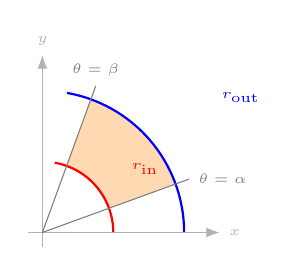
\begin{tikzpicture}[>=Latex,scale=0.9]
  \fill[orange!30,domain=20:70,samples=40,variable=\t]
    plot ({1.0*cos(\t)},{1.0*sin(\t)})
    -- plot[domain=70:20,samples=40,variable=\t] ({2.0*cos(\t)},{2.0*sin(\t)}) -- cycle;
  \draw[thick,blue,domain=0:80,samples=40] plot ({2.0*cos(\x)},{2.0*sin(\x)});
  \draw[thick,red,domain=0:80,samples=40] plot ({1.0*cos(\x)},{1.0*sin(\x)});
  \node[blue,font=\tiny] at (2.8,1.9){$r_{\rm out}$};
  \node[red,font=\tiny] at (1.45,0.9){$r_{\rm in}$};
  \draw[->,gray!60] (-0.2,0)--(2.5,0) node[right,font=\tiny]{$x$};
  \draw[->,gray!60] (0,-0.2)--(0,2.5) node[above,font=\tiny]{$y$};
  \draw[gray] (0,0) -- ({2.2*cos(20)},{2.2*sin(20)}) node[right,font=\tiny]{$\theta=\alpha$};
  \draw[gray] (0,0) -- ({2.2*cos(70)},{2.2*sin(70)}) node[above,font=\tiny]{$\theta=\beta$};
\end{tikzpicture}
\end{center}

\textbf{Arc length.}
\[
L = \int_\alpha^\beta \sqrt{r^2+\left(\frac{dr}{d\theta}\right)^2}\,d\theta
\]

\newpage

%                       --
\section{Chapter 12: Vectors and the Geometry of Space}
%                       --

\subsection{12.1 Three-Dimensional Coordinate Systems}

\begin{center}
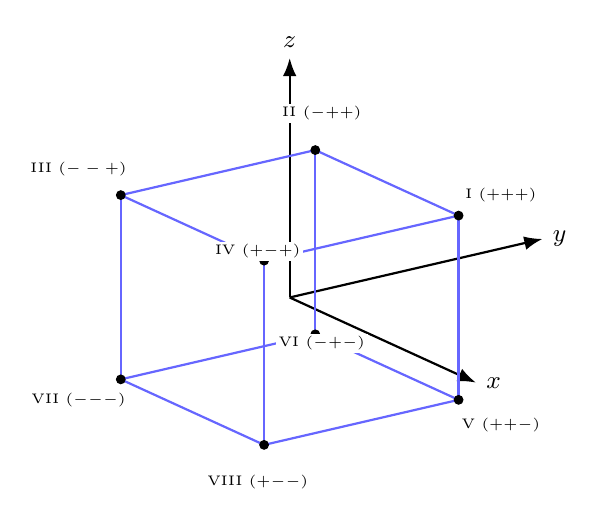
\begin{tikzpicture}[>=Latex,scale=1.3,x={(0.7cm,-0.32cm)},y={(0.95cm,0.22cm)},z={(0cm,0.9cm)}]
  % Axes
  \draw[->,thick] (0,0,0)--(2.6,0,0) node[right,font=\small]{$x$};
  \draw[->,thick] (0,0,0)--(0,2.6,0) node[right,font=\small]{$y$};
  \draw[->,thick] (0,0,0)--(0,0,2.6) node[above,font=\small]{$z$};
  % Cube edges centered at origin from (-1,-1,-1) to (1,1,1)
  \draw[blue!60,thick] (-1,-1,-1)--(1,-1,-1)--(1,1,-1)--(-1,1,-1)--cycle;
  \draw[blue!60,thick] (-1,-1,1)--(1,-1,1)--(1,1,1)--(-1,1,1)--cycle;
  \draw[blue!60,thick] (-1,-1,-1)--(-1,-1,1);
  \draw[blue!60,thick] (1,-1,-1)--(1,-1,1);
  \draw[blue!60,thick] (1,1,-1)--(1,1,1);
  \draw[blue!60,thick] (-1,1,-1)--(-1,1,1);
  % Vertex dots
  \foreach \sx in {-1,1} \foreach \sy in {-1,1} \foreach \sz in {-1,1}
    \filldraw[black] (\sx,\sy,\sz) circle (1.2pt);
  % Vertex labels (octant Roman + sign triple). Each label placed slightly outside the cube vertex.
  \node[font=\tiny,fill=white,inner sep=1pt] at (1.25,1.25,1.25){I $(+{+}{+})$};
  \node[font=\tiny,fill=white,inner sep=1pt] at (-1.25,1.25,1.25){II $(-{+}{+})$};
  \node[font=\tiny,fill=white,inner sep=1pt] at (-1.25,-1.25,1.25){III $(--{+})$};
  \node[font=\tiny,fill=white,inner sep=1pt] at (1.25,-1.25,1.25){IV $(+{-}{+})$};
  \node[font=\tiny,fill=white,inner sep=1pt] at (1.25,1.25,-1.25){V $(+{+}{-})$};
  \node[font=\tiny,fill=white,inner sep=1pt] at (-1.25,1.25,-1.25){VI $(-{+}{-})$};
  \node[font=\tiny,fill=white,inner sep=1pt] at (-1.25,-1.25,-1.25){VII $({-}{-}{-})$};
  \node[font=\tiny,fill=white,inner sep=1pt] at (1.25,-1.25,-1.25){VIII $({+}{-}{-})$};
\end{tikzpicture}
\end{center}

\textbf{Distance.} $|P_1P_2| = \sqrt{(x_2-x_1)^2+(y_2-y_1)^2+(z_2-z_1)^2}$.\quad
\textbf{Sphere.} $(x-h)^2+(y-k)^2+(z-l)^2=r^2$.

\medskip\textbf{Practice.}
\begin{enumerate}[noitemsep]
  \item Using only the 2D Pythagorean theorem (applied twice), find the distance from $(0,0,0)$ to $(1,1,1)$.
  \item Find the distance from the point $(4,-2,6)$ to each coordinate axis.
  \item Find the equation of a sphere if one of its diameters has endpoints $(2,1,4)$ and $(4,3,10)$.
\end{enumerate}

\subsection{12.2 Vectors}

\textbf{Vector.} something with magnitude and direction, $\vec{a} = \vv{a_1,a_2,a_3}$.

\textbf{Magnitude.} $|\vec{a}| = \sqrt{a_1^2+a_2^2+a_3^2}$

\textbf{Operations} (component-wise):
\[
\vec{a}+\vec{b} = \vv{a_1+b_1,\,a_2+b_2,\,a_3+b_3}, \qquad c\vec{a} = \vv{ca_1,ca_2,ca_3}
\]

\textbf{Unit vector.} $\hat{\vec{a}} = \vec{a}/|\vec{a}|$. standard basis $\ihat=\vv{1,0,0}$, $\jhat=\vv{0,1,0}$, $\khat=\vv{0,0,1}$.

\begin{center}
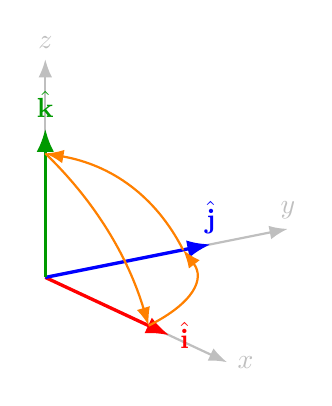
\begin{tikzpicture}[>=Latex,scale=1.4,x={(0.75cm,-0.35cm)},y={(1cm,0.2cm)},z={(0cm,0.9cm)}]
  % 3D axes with basis vectors (right-handed)
  \draw[->,gray!50,thick] (0,0,0) -- (2.2,0,0) node[right]{$x$};
  \draw[->,gray!50,thick] (0,0,0) -- (0,2.2,0) node[above]{$y$};
  \draw[->,gray!50,thick] (0,0,0) -- (0,0,2.2) node[above]{$z$};
  % Basis vectors (bold arrows from origin)
  \draw[->,very thick,red] (0,0,0) -- (1.5,0,0) node[right,red]{$\ihat$};
  \draw[->,very thick,blue] (0,0,0) -- (0,1.5,0) node[above,blue]{$\jhat$};
  \draw[->,very thick,green!60!black] (0,0,0) -- (0,0,1.5) node[above,green!60!black]{$\khat$};
  % Cyclic arrow: ihat -> jhat -> khat -> ihat (right-handed cycle, all bending outward from origin)
  \draw[->,thick,orange] (1.25,0,0) .. controls (1.0,0.6,0) and (0.6,1.0,0) .. (0,1.25,0);
  \draw[->,thick,orange] (0,1.25,0) .. controls (0,1.0,0.6) and (0,0.6,1.0) .. (0,0,1.25);
  \draw[->,thick,orange] (0,0,1.25) .. controls (0.6,0,1.0) and (1.0,0,0.6) .. (1.25,0,0);
\end{tikzpicture}
\end{center}

cyclic relations $\ihat\times\jhat=\khat$, $\jhat\times\khat=\ihat$, $\khat\times\ihat=\jhat$.

\begin{center}
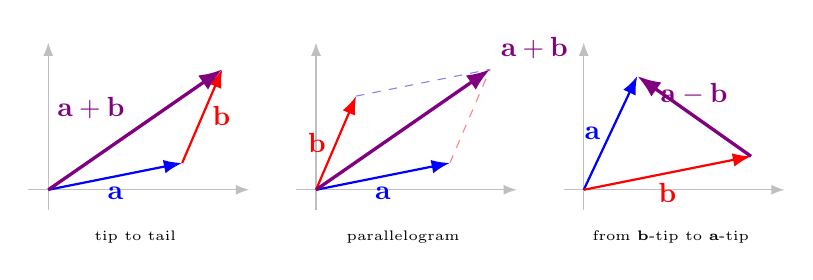
\begin{tikzpicture}[>=Latex,scale=0.85]
  % Addition (tip to tail)
  \begin{scope}
    \draw[->,gray!50] (-0.3,0)--(3,0); \draw[->,gray!50] (0,-0.3)--(0,2.2);
    \draw[->,thick,blue] (0,0)--(2,0.4) node[midway,below,blue]{$\vec a$};
    \draw[->,thick,red] (2,0.4)--(2.6,1.8) node[midway,right,red]{$\vec b$};
    \draw[->,very thick,violet] (0,0)--(2.6,1.8) node[midway,above left,violet]{$\vec a+\vec b$};
    \node[font=\tiny] at (1.3,-0.7){tip to tail};
  \end{scope}
  % Addition parallelogram law
  \begin{scope}[xshift=4cm]
    \draw[->,gray!50] (-0.3,0)--(3,0); \draw[->,gray!50] (0,-0.3)--(0,2.2);
    \draw[->,thick,blue] (0,0)--(2,0.4) node[midway,below,blue]{$\vec a$};
    \draw[->,thick,red] (0,0)--(0.6,1.4) node[midway,left,red]{$\vec b$};
    \draw[dashed,blue!50] (0.6,1.4)--(2.6,1.8);
    \draw[dashed,red!50] (2,0.4)--(2.6,1.8);
    \draw[->,very thick,violet] (0,0)--(2.6,1.8) node[above right,violet]{$\vec a+\vec b$};
    \node[font=\tiny] at (1.3,-0.7){parallelogram};
  \end{scope}
  % Subtraction (tip to tip)
  \begin{scope}[xshift=8cm]
    \draw[->,gray!50] (-0.3,0)--(3,0); \draw[->,gray!50] (0,-0.3)--(0,2.2);
    \draw[->,thick,blue] (0,0)--(0.8,1.7) node[midway,left,blue]{$\vec a$};
    \draw[->,thick,red] (0,0)--(2.5,0.5) node[midway,below,red]{$\vec b$};
    \draw[->,very thick,violet] (2.5,0.5)--(0.8,1.7) node[midway,above,violet]{$\vec a-\vec b$};
    \node[font=\tiny] at (1.3,-0.7){from $\vec b$-tip to $\vec a$-tip};
  \end{scope}
\end{tikzpicture}

\medskip

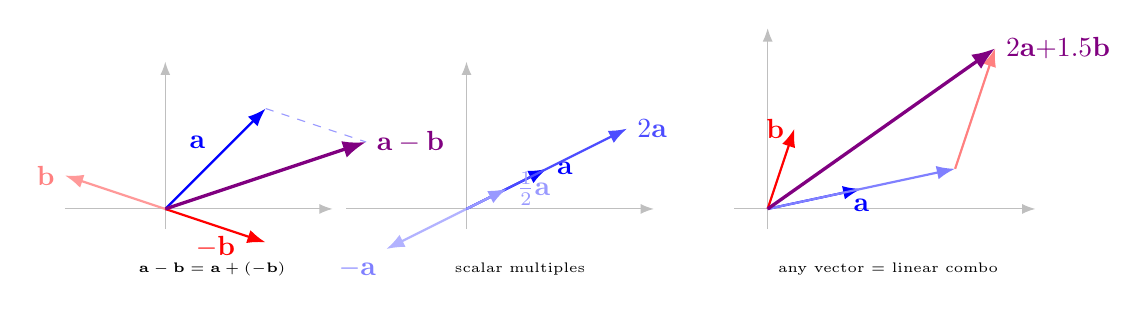
\begin{tikzpicture}[>=Latex,scale=0.85]
  % Subtraction as a + (-b)
  \begin{scope}
    \draw[->,gray!50] (-1.5,0)--(2.5,0); \draw[->,gray!50] (0,-0.3)--(0,2.2);
    \draw[->,thick,blue] (0,0)--(1.5,1.5) node[midway,above left,blue]{$\vec a$};
    \draw[->,thick,red] (0,0)--(1.5,-0.5) node[midway,below,red]{$-\vec b$};
    \draw[->,thick,red!40] (0,0)--(-1.5,0.5) node[left,red!50]{$\vec b$};
    \draw[->,very thick,violet] (0,0)--(3.0,1.0) node[right,violet]{$\vec a-\vec b$};
    \draw[dashed,blue!40] (1.5,1.5)--(3.0,1.0);
    \node[font=\tiny] at (0.7,-0.9){$\vec a-\vec b=\vec a+(-\vec b)$};
  \end{scope}
  % Scalar multiples
  \begin{scope}[xshift=4.5cm]
    \draw[->,gray!50] (-1.8,0)--(2.8,0); \draw[->,gray!50] (0,-0.3)--(0,2.2);
    \draw[->,thick,blue!30] (0,0)--(-1.2,-0.6) node[below left,blue!50]{$-\vec a$};
    \draw[->,thick,blue] (0,0)--(1.2,0.6) node[right,blue]{$\vec a$};
    \draw[->,thick,blue!70] (0,0)--(2.4,1.2) node[right,blue!70]{$2\vec a$};
    \draw[->,thick,blue!40] (0,0)--(0.6,0.3) node[right,blue!40]{$\tfrac12\vec a$};
    \node[font=\tiny] at (0.8,-0.9){scalar multiples};
  \end{scope}
  % Linear combination
  \begin{scope}[xshift=9cm]
    \draw[->,gray!50] (-0.5,0)--(4,0); \draw[->,gray!50] (0,-0.3)--(0,2.7);
    \draw[->,thick,blue] (0,0)--(1.4,0.3) node[below,blue]{$\vec a$};
    \draw[->,thick,red] (0,0)--(0.4,1.2) node[left,red]{$\vec b$};
    \draw[->,thick,blue!50] (0,0)--(2.8,0.6);
    \draw[->,thick,red!50] (2.8,0.6)--(3.4,2.4);
    \draw[->,very thick,violet] (0,0)--(3.4,2.4) node[right,violet]{$2\vec a{+}1.5\vec b$};
    \node[font=\tiny] at (1.8,-0.9){any vector $=$ linear combo};
  \end{scope}
\end{tikzpicture}

\medskip

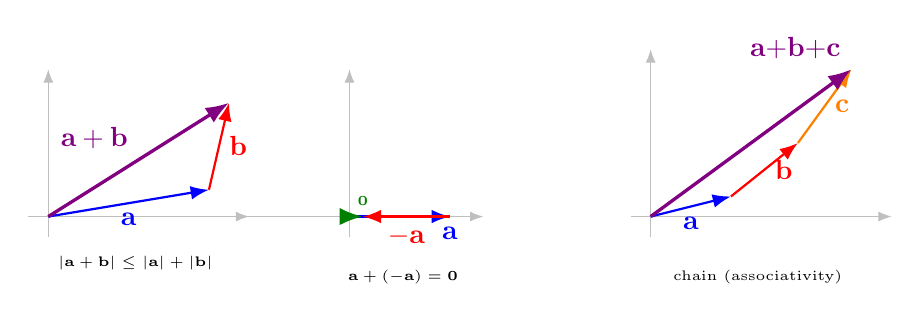
\begin{tikzpicture}[>=Latex,scale=0.85]
  % Triangle inequality
  \begin{scope}
    \draw[->,gray!50] (-0.3,0)--(3,0); \draw[->,gray!50] (0,-0.3)--(0,2.2);
    \draw[->,thick,blue] (0,0)--(2.4,0.4) node[midway,below,blue]{$\vec a$};
    \draw[->,thick,red] (2.4,0.4)--(2.7,1.7) node[midway,right,red]{$\vec b$};
    \draw[->,very thick,violet] (0,0)--(2.7,1.7) node[midway,above left,violet]{$\vec a+\vec b$};
    \node[font=\tiny] at (1.3,-0.7){$|\vec a+\vec b|\le|\vec a|+|\vec b|$};
  \end{scope}
  % Anti-parallel cancellation
  \begin{scope}[xshift=4.5cm]
    \draw[->,gray!50] (-2,0)--(2,0); \draw[->,gray!50] (0,-0.3)--(0,2.2);
    \draw[->,thick,blue] (0,0)--(1.5,0) node[below,blue]{$\vec a$};
    \draw[->,thick,red] (1.5,0)--(0.2,0) node[midway,below,red]{$-\vec a$};
    \draw[->,thick,green!50!black,very thick] (0,0)--(0.2,0) node[above,green!50!black,font=\tiny]{$\vec 0$};
    \node[font=\tiny] at (0.8,-0.9){$\vec a+(-\vec a)=\vec 0$};
  \end{scope}
  % Chain of three vectors
  \begin{scope}[xshift=9cm]
    \draw[->,gray!50] (-0.3,0)--(3.6,0); \draw[->,gray!50] (0,-0.3)--(0,2.5);
    \draw[->,thick,blue] (0,0)--(1.2,0.3) node[midway,below,blue]{$\vec a$};
    \draw[->,thick,red] (1.2,0.3)--(2.2,1.1) node[midway,right,red]{$\vec b$};
    \draw[->,thick,orange] (2.2,1.1)--(3.0,2.2) node[midway,right,orange]{$\vec c$};
    \draw[->,very thick,violet] (0,0)--(3.0,2.2) node[above left,violet]{$\vec a{+}\vec b{+}\vec c$};
    \node[font=\tiny] at (1.6,-0.9){chain (associativity)};
  \end{scope}
\end{tikzpicture}
\end{center}

\textit{Same idea in 3D.}

\begin{center}
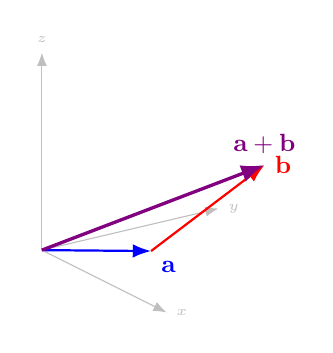
\begin{tikzpicture}[>=Latex,scale=1.2,x={(0.6cm,-0.3cm)},y={(0.85cm,0.2cm)},z={(0cm,0.95cm)}]
  \draw[->,gray!50] (0,0,0)--(2.2,0,0) node[right,font=\tiny]{$x$};
  \draw[->,gray!50] (0,0,0)--(0,2.2,0) node[right,font=\tiny]{$y$};
  \draw[->,gray!50] (0,0,0)--(0,0,2.2) node[above,font=\tiny]{$z$};
  \draw[->,thick,blue] (0,0,0)--(1.5,0.3,0.4) node[below right,font=\small]{$\vec a$};
  \draw[->,thick,red] (1.5,0.3,0.4)--(1.5+0.3,0.3+1.2,0.4+0.8) node[right,font=\small]{$\vec b$};
  \draw[->,very thick,violet] (0,0,0)--(1.8,1.5,1.2) node[above,font=\small]{$\vec a+\vec b$};
\end{tikzpicture}
\end{center}

\medskip\textbf{Practice.}
\begin{enumerate}[noitemsep]
  \item Find a vector parallel to the line $y=2x+1$.
  \item A 2D vector has magnitude $2$ and makes an angle of $\pi/4$ with the positive $x$-axis. Express it in $a\ihat+b\jhat$ form and find a unit vector in the same direction.
  \item Find the unit vector in the direction from $P(1,2,3)$ to $Q(4,6,3)$.
\end{enumerate}

\subsection{12.3 The Dot Product}

\textbf{Dot product.} $\vec{a}\cdot\vec{b} = a_1b_1+a_2b_2+a_3b_3$

\begin{thm}[Geometric formula]
$\vec{a}\cdot\vec{b} = |\vec{a}||\vec{b}|\cos\theta$ where $\theta\in[0,\pi]$ is the angle between the vectors.
\end{thm}

\textbf{Orthogonality.} $\vec{a}\perp\vec{b} \iff \vec{a}\cdot\vec{b}=0$

\textbf{Direction angles/cosines.}
\[
\cos\alpha = \frac{a_1}{|\vec{a}|},\quad \cos\beta = \frac{a_2}{|\vec{a}|},\quad \cos\gamma = \frac{a_3}{|\vec{a}|}; \qquad \cos^2\alpha+\cos^2\beta+\cos^2\gamma=1
\]

\textbf{Scalar projection.} $\text{comp}_{\vec{a}}\vec{b} = \dfrac{\vec{a}\cdot\vec{b}}{|\vec{a}|}$ \qquad
\textbf{Vector projection.} $\text{proj}_{\vec{a}}\vec{b} = \dfrac{\vec{a}\cdot\vec{b}}{|\vec{a}|^2}\,\vec{a}$

\begin{center}
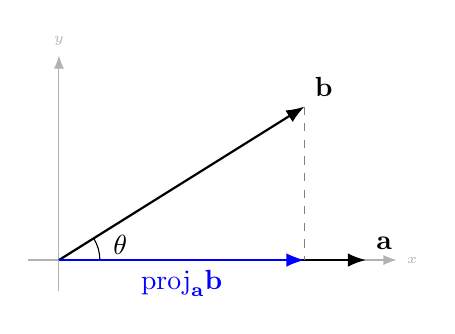
\begin{tikzpicture}[>=Latex,scale=1.3]
  \draw[->,gray!60] (-0.3,0)--(3.3,0) node[right,font=\tiny]{$x$};
  \draw[->,gray!60] (0,-0.3)--(0,2.0) node[above,font=\tiny]{$y$};
  \draw[->,thick] (0,0) -- (3,0) node[above right] {$\vec{a}$};
  \draw[->,thick] (0,0) -- (2.4,1.5) node[above right] {$\vec{b}$};
  \draw[dashed,gray] (2.4,1.5) -- (2.4,0);
  \draw[->,blue,thick] (0,0) -- (2.4,0) node[midway,below,blue] {$\mathrm{proj}_{\vec{a}}\vec{b}$};
  \draw (0.4,0) arc (0:32:0.4);
  \node at (0.6,0.15) {$\theta$};
\end{tikzpicture}
\end{center}

\textit{3D version, same projection idea.}

\begin{center}
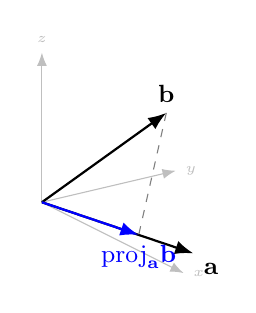
\begin{tikzpicture}[>=Latex,scale=1.0,x={(0.6cm,-0.3cm)},y={(0.85cm,0.2cm)},z={(0cm,0.95cm)}]
  \draw[->,gray!50] (0,0,0)--(3,0,0) node[right,font=\tiny]{$x$};
  \draw[->,gray!50] (0,0,0)--(0,2,0) node[right,font=\tiny]{$y$};
  \draw[->,gray!50] (0,0,0)--(0,0,2) node[above,font=\tiny]{$z$};
  \draw[->,thick] (0,0,0)--(2.5,0.5,0) node[below right,font=\small]{$\vec a$};
  \draw[->,thick] (0,0,0)--(1.5,0.8,1.5) node[above,font=\small]{$\vec b$};
  % projection of b onto a direction
  \pgfmathsetmacro{\nrm}{sqrt(2.5*2.5+0.5*0.5)}
  \pgfmathsetmacro{\dotv}{(1.5*2.5+0.8*0.5+1.5*0)/(\nrm*\nrm)}
  \draw[->,blue,thick] (0,0,0)--({2.5*\dotv},{0.5*\dotv},0) node[below,font=\small,blue]{$\mathrm{proj}_{\vec a}\vec b$};
  \draw[dashed,gray] (1.5,0.8,1.5)--({2.5*\dotv},{0.5*\dotv},0);
\end{tikzpicture}
\end{center}

\textbf{Work.} $W = \vec{F}\cdot\vec{D} = |\vec{F}||\vec{D}|\cos\theta$.

\textit{Geometrically.} dot product is length of projection of one vector onto the other.

\medskip\textbf{Practice.}
\begin{enumerate}[noitemsep]
  \item Find the angle $\theta$ between $\vec{u}=\langle 1,\sqrt{3}\rangle$ and $\vec{v}=\langle 1,0\rangle$.
  \item Determine whether $\vec{u}=\langle 2,6,-4\rangle$ and $\vec{v}=\langle -3,1,0\rangle$ are orthogonal, parallel, or neither.
  \item If $\vec{a}=\langle 1,1\rangle$ and $\vec{b}=\langle -1,2\rangle$, draw and calculate $\mathrm{proj}_{\vec{a}}\vec{b}$ and $\mathrm{orth}_{\vec{a}}\vec{b}$.
\end{enumerate}

\subsection{12.4 The Cross Product}

\textbf{Cross product.}
\[
\vec{a}\times\vec{b} = \begin{vmatrix}\ihat & \jhat & \khat \\ a_1 & a_2 & a_3 \\ b_1 & b_2 & b_3\end{vmatrix} = \vv{a_2b_3-a_3b_2,\; a_3b_1-a_1b_3,\; a_1b_2-a_2b_1}
\]

\textbf{Determinants and areas/volumes.} A $2\times 2$ determinant $\begin{vmatrix}a&b\\c&d\end{vmatrix} = ad-bc$ gives the signed area of the parallelogram spanned by $(a,c)$ and $(b,d)$. The $3\times 3$ determinant $\det\begin{pmatrix}a_1&a_2&a_3\\b_1&b_2&b_3\\c_1&c_2&c_3\end{pmatrix}$ gives the signed volume of the parallelepiped spanned by $\vec{a},\vec{b},\vec{c}$.

\textit{Derivation of $|ad-bc|$.} Span the parallelogram by $\vec u=(a,b)$ and $\vec v=(c,d)$. Enclose it in the $(a+c)\times(b+d)$ bounding rectangle and subtract the corner pieces (2 small rectangles of area $bc$ each and 4 right triangles whose pairs sum to $ab$ and $cd$):
\[
\text{Area}=(a+c)(b+d)-2bc-ab-cd=ab+ad+bc+cd-2bc-ab-cd=ad-bc.
\]

\begin{center}
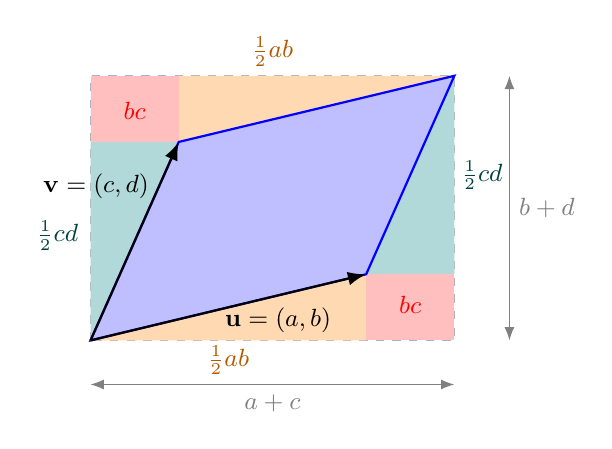
\begin{tikzpicture}[>=Latex,scale=1.4]
  % Bounding rectangle + parallelogram decomposition: u=(a,b)=(2.5,0.6), v=(c,d)=(0.8,1.8)
  \coordinate (O) at (0,0);
  \coordinate (U) at (2.5,0.6);
  \coordinate (V) at (0.8,1.8);
  \coordinate (UV) at (3.3,2.4);
  \draw[gray!60,dashed] (0,0) rectangle (3.3,2.4);
  % Corner triangles & rectangles (faintly shaded)
  \fill[orange!30] (0,0)--(U)--(2.5,0)--cycle;
  \fill[orange!30] (V)--(UV)--(0.8,2.4)--cycle;
  \fill[teal!30] (0,0)--(V)--(0,1.8)--cycle;
  \fill[teal!30] (U)--(UV)--(3.3,0.6)--cycle;
  \fill[red!25] (2.5,0)--(3.3,0)--(3.3,0.6)--(2.5,0.6)--cycle;
  \fill[red!25] (0,1.8)--(0.8,1.8)--(0.8,2.4)--(0,2.4)--cycle;
  % Parallelogram
  \fill[blue!25] (O)--(U)--(UV)--(V)--cycle;
  \draw[blue,thick] (O)--(U)--(UV)--(V)--cycle;
  \draw[->,thick] (O)--(U);
  \draw[->,thick] (O)--(V);
  % Vector labels placed clear
  \node[font=\small] at (1.7,0.18){$\vec u=(a,b)$};
  \node[font=\small] at (0.05,1.4){$\vec v=(c,d)$};
  % Side dimensions
  \draw[<->,gray] (0,-0.4)--(3.3,-0.4) node[midway,below,font=\small]{$a+c$};
  \draw[<->,gray] (3.8,0)--(3.8,2.4) node[midway,right,font=\small]{$b+d$};
  % Piece labels — well separated outside the rectangle
  \node[red,font=\small] at (2.9,0.32){$bc$};
  \node[red,font=\small] at (0.4,2.08){$bc$};
  \node[orange!70!black,font=\small] at (1.25,-0.18){$\tfrac12 ab$};
  \node[orange!70!black,font=\small] at (1.65,2.62){$\tfrac12 ab$};
  \node[teal!50!black,font=\small] at (-0.3,0.95){$\tfrac12 cd$};
  \node[teal!50!black,font=\small] at (3.55,1.5){$\tfrac12 cd$};
\end{tikzpicture}
\end{center}

\textit{Sign of $ad-bc$.} If $\vec u$ to $\vec v$ goes counterclockwise, $ad-bc>0$; if clockwise, $ad-bc<0$. The unsigned area is $|ad-bc|$.

\begin{center}
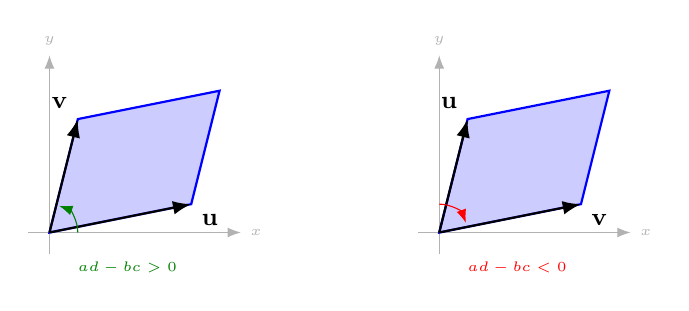
\begin{tikzpicture}[>=Latex,scale=0.9]
  % Positive orientation (CCW from u to v)
  \begin{scope}
    \draw[->,gray!60](-0.3,0)--(2.7,0)node[right,font=\tiny]{$x$};
    \draw[->,gray!60](0,-0.3)--(0,2.5)node[above,font=\tiny]{$y$};
    \fill[blue!20] (0,0)--(2,0.4)--(2.4,2.0)--(0.4,1.6)--cycle;
    \draw[blue,thick] (0,0)--(2,0.4)--(2.4,2.0)--(0.4,1.6)--cycle;
    \draw[->,thick] (0,0)--(2,0.4) node[below right,font=\small]{$\vec u$};
    \draw[->,thick] (0,0)--(0.4,1.6) node[above left,font=\small]{$\vec v$};
    \draw[->,green!50!black] (0.4,0) arc (0:70:0.4);
    \node[green!50!black,font=\tiny] at (1.1,-0.5){$ad-bc>0$};
  \end{scope}
  % Negative orientation
  \begin{scope}[xshift=5.5cm]
    \draw[->,gray!60](-0.3,0)--(2.7,0)node[right,font=\tiny]{$x$};
    \draw[->,gray!60](0,-0.3)--(0,2.5)node[above,font=\tiny]{$y$};
    \fill[blue!20] (0,0)--(0.4,1.6)--(2.4,2.0)--(2,0.4)--cycle;
    \draw[blue,thick] (0,0)--(0.4,1.6)--(2.4,2.0)--(2,0.4)--cycle;
    \draw[->,thick] (0,0)--(0.4,1.6) node[above left,font=\small]{$\vec u$};
    \draw[->,thick] (0,0)--(2,0.4) node[below right,font=\small]{$\vec v$};
    \draw[->,red] (0,0.4) arc (90:20:0.4);
    \node[red,font=\tiny] at (1.1,-0.5){$ad-bc<0$};
  \end{scope}
\end{tikzpicture}
\end{center}

\textit{check.} For $\vec u=(1,0)$, $\vec v=(0,1)$: $ad-bc=1\cdot 1-0\cdot 0=1$ — the unit square has area 1, CCW orientation.

\begin{center}
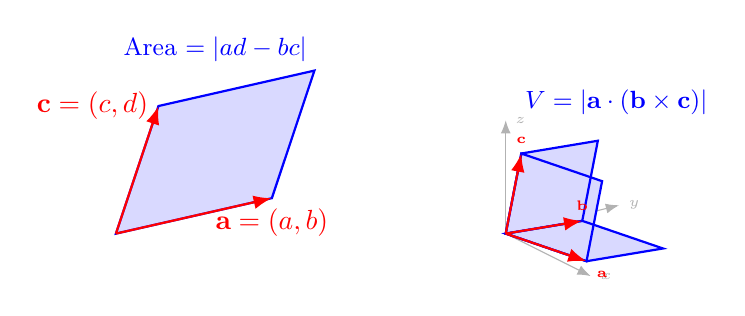
\begin{tikzpicture}[>=Latex,scale=0.9]
  % 2D parallelogram: vec a = (a,b), vec c = (c,d)
  \begin{scope}
    \coordinate (a) at (2.2,0.5);
    \coordinate (c) at (0.6,1.8);
    \filldraw[blue!15] (0,0) -- (a) -- ($(a)+(c)$) -- (c) -- cycle;
    \draw[blue,thick] (0,0) -- (a) -- ($(a)+(c)$) -- (c) -- cycle;
    \draw[->,thick,red] (0,0) -- (a) node[below]{$\vec a=(a,b)$};
    \draw[->,thick,red] (0,0) -- (c) node[left]{$\vec c=(c,d)$};
    \node[blue,font=\small,align=center] at (1.4,2.6){Area $=|ad-bc|$};
  \end{scope}
  % 3D parallelepiped
  \begin{scope}[xshift=5.5cm,x={(0.6cm,-0.3cm)},y={(0.8cm,0.2cm)},z={(0cm,0.8cm)}]
    \draw[->,gray!60,thin] (0,0,0) -- (2,0,0) node[right,font=\tiny]{$x$};
    \draw[->,gray!60,thin] (0,0,0) -- (0,2,0) node[right,font=\tiny]{$y$};
    \draw[->,gray!60,thin] (0,0,0) -- (0,0,2) node[right,font=\tiny]{$z$};
    \coordinate (va) at (1.5,0.3,0);
    \coordinate (vb) at (0.2,1.2,0);
    \coordinate (vc) at (0.1,0.2,1.4);
    \fill[blue!15] (0,0,0) -- (va) -- ($(va)+(vb)$) -- (vb) -- cycle;
    \fill[blue!15] (0,0,0) -- (va) -- ($(va)+(vc)$) -- (vc) -- cycle;
    \fill[blue!15] (0,0,0) -- (vb) -- ($(vb)+(vc)$) -- (vc) -- cycle;
    \draw[blue,thick] (0,0,0) -- (va) -- ($(va)+(vb)$) -- (vb) -- cycle;
    \draw[blue,thick] (0,0,0) -- (vc) -- ($(vc)+(va)$) -- (va) -- cycle;
    \draw[blue,thick] (0,0,0) -- (vc) -- ($(vc)+(vb)$) -- (vb) -- cycle;
    \draw[->,thick,red] (0,0,0) -- (va) node[below right,font=\tiny]{$\vec a$};
    \draw[->,thick,red] (0,0,0) -- (vb) node[above,font=\tiny]{$\vec b$};
    \draw[->,thick,red] (0,0,0) -- (vc) node[above,font=\tiny]{$\vec c$};
    \node[blue,font=\small,align=center] at (1.0,1.2,2.4){$V = |\vec a \cdot (\vec b \times \vec c)|$};
  \end{scope}
\end{tikzpicture}
\end{center}

cofactor expansion along the top row
\[
\det\begin{pmatrix}\ihat&\jhat&\khat\\a_1&a_2&a_3\\b_1&b_2&b_3\end{pmatrix} = \ihat(a_2b_3-a_3b_2) - \jhat(a_1b_3-a_3b_1) + \khat(a_1b_2-a_2b_1) = \vec{a}\times\vec{b}.
\]

\textbf{Perpendicularity.} check $(\vec{a}\times\vec{b})\cdot\vec{a}=0$ by expanding.
\begin{align*}
(\vec{a}\times\vec{b})\cdot\vec{a} &= (a_2b_3-a_3b_2)a_1 - (a_1b_3-a_3b_1)a_2 + (a_1b_2-a_2b_1)a_3\\
&= a_1a_2b_3 - a_1a_3b_2 - a_1a_2b_3 + a_2a_3b_1 + a_1a_3b_2 - a_2a_3b_1 = 0.
\end{align*}
same for $\vec b$. any vector perpendicular to both $\vec a$ and $\vec b$ (when not parallel) is a scalar multiple of $\vec a\times\vec b$.

\textbf{Properties.}
\begin{itemize}[noitemsep]
\item $\vec{a}\times\vec{b}$ is perpendicular to both $\vec{a}$ and $\vec{b}$ (right-hand rule gives direction)
\item $|\vec{a}\times\vec{b}| = |\vec{a}||\vec{b}|\sin\theta$
\item $\vec{a}\parallel\vec{b} \iff \vec{a}\times\vec{b} = \vec{0}$
\item $\vec{a}\times\vec{b} = -\vec{b}\times\vec{a}$ (anticommutative)
\end{itemize}

\textbf{Areas.} parallelogram $= |\vec{a}\times\vec{b}|$. triangle $= \tfrac{1}{2}|\vec{a}\times\vec{b}|$.

\begin{center}
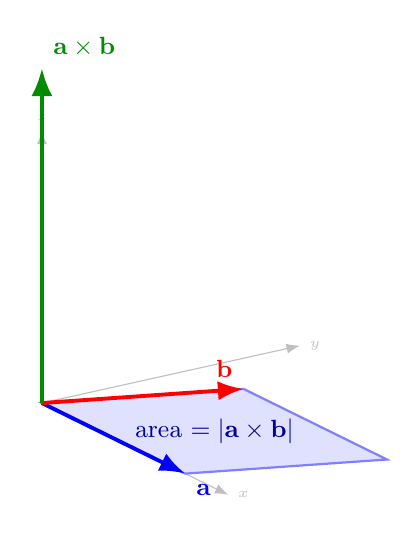
\begin{tikzpicture}[>=Latex,scale=1.4,x={(0.65cm,-0.32cm)},y={(0.9cm,0.2cm)},z={(0cm,0.95cm)}]
  \draw[->,gray!50] (0,0,0)--(2.6,0,0) node[right,font=\tiny]{$x$};
  \draw[->,gray!50] (0,0,0)--(0,2.6,0) node[right,font=\tiny]{$y$};
  \draw[->,gray!50] (0,0,0)--(0,0,2.6) node[above,font=\tiny]{$z$};
  % a along x.  b at angle in xy-plane.
  \pgfmathsetmacro{\ax}{2.0}\pgfmathsetmacro{\ay}{0.0}
  \pgfmathsetmacro{\bx}{0.6}\pgfmathsetmacro{\by}{1.6}
  % parallelogram in the xy plane.  axb is perpendicular pointing along +z.
  \fill[blue!12] (0,0,0) -- (\ax,\ay,0) -- (\ax+\bx,\ay+\by,0) -- (\bx,\by,0) -- cycle;
  \draw[blue!50,thick] (0,0,0) -- (\ax,\ay,0) -- (\ax+\bx,\ay+\by,0) -- (\bx,\by,0) -- cycle;
  % a and b
  \draw[->,line width=1.4pt,blue] (0,0,0) -- (\ax,\ay,0) node[below right,blue,font=\small]{$\vec a$};
  \draw[->,line width=1.4pt,red]  (0,0,0) -- (\bx,\by,0) node[above left,red,font=\small]{$\vec b$};
  % a x b straight up.   length = |a||b| sin theta which here is 2 * sqrt(b_x^2+b_y^2) * sin angle.
  \pgfmathsetmacro{\axbLen}{\ax * \by - \ay * \bx}
  \draw[->,line width=1.6pt,green!55!black] (0,0,0) -- (0,0,{\axbLen})
    node[above right,green!55!black,font=\small]{$\vec a\times\vec b$};
  % area label in the middle of the parallelogram
  \node[blue!60!black,font=\small] at ({(\ax+\bx)/2},{(\ay+\by)/2},0){area $= |\vec a\times\vec b|$};
\end{tikzpicture}
\end{center}

$|\vec a\times\vec b|$ is the area of the parallelogram. direction is perp by the right hand rule.

\textit{Right hand rule.} curl your right-hand fingers from $\vec a$ toward $\vec b$. your thumb points along $\vec a\times\vec b$.

\begin{center}
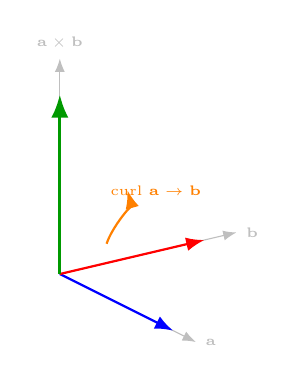
\begin{tikzpicture}[>=Latex,scale=1.2,x={(0.6cm,-0.3cm)},y={(0.85cm,0.2cm)},z={(0cm,0.95cm)}]
  \draw[->,gray!50] (0,0,0)--(2.4,0,0) node[right,font=\tiny]{$\vec a$};
  \draw[->,gray!50] (0,0,0)--(0,2.2,0) node[right,font=\tiny]{$\vec b$};
  \draw[->,gray!50] (0,0,0)--(0,0,2.4) node[above,font=\tiny]{$\vec a\times\vec b$};
  % Vectors
  \draw[->,thick,blue] (0,0,0)--(2,0,0);
  \draw[->,thick,red] (0,0,0)--(0,1.8,0);
  \draw[->,thick,green!60!black,very thick] (0,0,0)--(0,0,2);
  % Curling arc from a to b
  \draw[->,orange,thick] (0.4,0.3,0.4) .. controls (0.7,0.15,0.7) and (0.55,0.5,0.85) .. (0.2,0.7,0.85);
  \node[orange,font=\tiny] at (0.7,0.7,1.0){curl $\vec a\to\vec b$};
\end{tikzpicture}
\end{center}

\textbf{Scalar triple product.} $\vec{a}\cdot(\vec{b}\times\vec{c}) = \det\begin{pmatrix}a_1&a_2&a_3\\b_1&b_2&b_3\\c_1&c_2&c_3\end{pmatrix}$.

\textbf{Volume of parallelepiped.} $V = |\vec{a}\cdot(\vec{b}\times\vec{c})|$.

\textbf{Torque.} $\vec{\tau} = \vec{r}\times\vec{F}$, magnitude $|\vec r||\vec F|\sin\theta$, force times moment arm.

\medskip\textbf{Practice.}
\begin{enumerate}[noitemsep]
  \item Determine each of the following without explicit computation: $\ihat\times\jhat$,\ $\jhat\times\khat$,\ $\khat\times\ihat$,\ and $-2\khat\times\jhat$.
  \item Find the cross product $\vec{a}\times\vec{b}$ for $\vec{a}=\langle 1,3,-2\rangle$ and $\vec{b}=\langle 2,1,1\rangle$.
  \item Find a unit vector orthogonal to both $\vec{u}=\langle 1,1,0\rangle$ and $\vec{v}=\langle 0,1,1\rangle$.
\end{enumerate}

\subsection{12.5 Equations of Lines and Planes}

\textbf{Line through $P_0=(x_0,y_0,z_0)$ with direction $\vec{v}=\vv{a,b,c}$:}
\begin{align*}
\text{Vector:}\quad & \vec{r} = \vec{r}_0 + t\vec{v}\\
\text{Parametric:}\quad & x=x_0+at,\; y=y_0+bt,\; z=z_0+ct\\
\text{Symmetric:}\quad & \frac{x-x_0}{a}=\frac{y-y_0}{b}=\frac{z-z_0}{c}
\end{align*}

\textbf{Skew lines.} non-parallel, non-intersecting (exist only in $\R^3$).

\textbf{Plane through $P_0$ with normal $\vec{n}=\vv{a,b,c}$:}
\[
\vec{n}\cdot(\vec{r}-\vec{r}_0)=0, \qquad a(x-x_0)+b(y-y_0)+c(z-z_0)=0
\]

\textbf{Distance from $P$ to plane.} Pick \emph{any} point $Q_0$ on the plane; project $\overrightarrow{Q_0P}$ onto unit normal $\hat{\vec n}$:
\[
D = \bigl|\overrightarrow{Q_0P}\cdot\hat{\vec{n}}\bigr| = \frac{|ax_1+by_1+cz_1+d|}{\sqrt{a^2+b^2+c^2}}
\]

\begin{center}
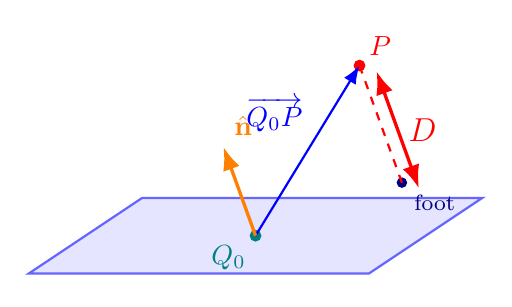
\begin{tikzpicture}[>=Latex,scale=1.2]
  % Plane lying mostly flat with a slight tilt.  parameter the plane as
  % { Q_0 + s u + t v }  with u = (1.6, -0.05), v = (0.7, 0.45)
  % so normal n = u x v has its 2-d projection nearly vertical.
  \coordinate (Q) at (1.6, 0.7);
  \coordinate (P) at (2.7, 2.5);
  \fill[blue!10]   ($(Q)+(-1.8,0)+(-0.6,-0.4)$) --
                   ($(Q)+( 1.8,0)+(-0.6,-0.4)$) --
                   ($(Q)+( 1.8,0)+( 0.6, 0.4)$) --
                   ($(Q)+(-1.8,0)+( 0.6, 0.4)$) -- cycle;
  \draw[blue!60,thick]
                   ($(Q)+(-1.8,0)+(-0.6,-0.4)$) --
                   ($(Q)+( 1.8,0)+(-0.6,-0.4)$) --
                   ($(Q)+( 1.8,0)+( 0.6, 0.4)$) --
                   ($(Q)+(-1.8,0)+( 0.6, 0.4)$) -- cycle;
  % The foot of the perpendicular from P to the plane.  Plane's 2-d normal
  % direction (-0.36, 1) normalised then projected.
  \pgfmathsetmacro{\nhx}{-0.34}\pgfmathsetmacro{\nhy}{0.94}
  \pgfmathsetmacro{\dval}{(2.7-1.6)*\nhx + (2.5-0.7)*\nhy}
  \coordinate (foot) at ($(P)-(\dval*\nhx,\dval*\nhy)$);
  % Q0 and P points
  \filldraw[teal] (Q) circle (1.6pt) node[below left,teal]{$Q_0$};
  \filldraw[red]  (P) circle (1.6pt) node[above right,red]{$P$};
  \filldraw[blue!50!black] (foot) circle (1.4pt) node[below right=1pt,font=\footnotesize]{foot};
  % Q_0 P vector
  \draw[->,thick,blue] (Q) -- (P) node[pos=0.55,above left,blue]{$\overrightarrow{Q_0P}$};
  % Unit normal n hat from Q_0, pointing into the half-space containing P
  \draw[->,very thick,orange] (Q) -- ($(Q)+(\nhx,\nhy)$) node[above right,orange]{$\hat{\vec n}$};
  % Perpendicular distance D from P down to the foot
  \draw[dashed,red,thick] (P) -- (foot);
  \draw[<->,red,very thick] ($(P)+(0.18,-0.06)$) -- ($(foot)+(0.18,-0.06)$)
    node[pos=0.5,right,red,font=\large\bfseries]{$D$};
\end{tikzpicture}
\end{center}

\textit{Picture.} drop a perpendicular from $P$ to the plane; its length $D$ equals the projection of $\overrightarrow{Q_0P}$ onto the unit normal $\hat{\vec n}$.

\textbf{Angle between planes} = angle between their normals.

\textbf{Distance from $P$ to line.} Let the line pass through point $Q$ with direction $\vec{v}$. Two methods:

\textit{Method 1.} $D = |\mathrm{orth}_{\vec{v}}\,\overrightarrow{QP}| = \sqrt{|\overrightarrow{QP}|^2 - |\mathrm{proj}_{\vec{v}}\,\overrightarrow{QP}|^2}$ \quad (orthogonal projection)

\textit{Method 2.} $D = \dfrac{|\overrightarrow{QP}\times\vec{v}|}{|\vec{v}|}$ \quad (derived from $|\overrightarrow{QP}\times\vec{v}| = |\overrightarrow{QP}||\vec{v}|\sin\theta$, where $\sin\theta \cdot |\overrightarrow{QP}| = D$)

\begin{center}
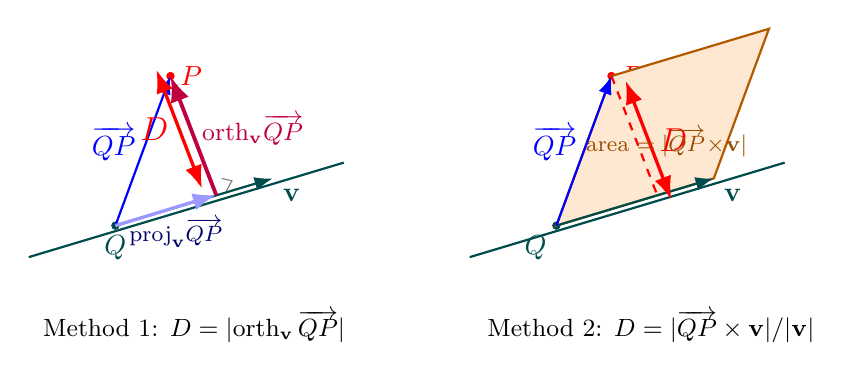
\begin{tikzpicture}[>=Latex,scale=1.0]
  % Left: Method 1 — D = | orth_v QP | as the perpendicular component
  \begin{scope}
    \node[font=\small,below] at (1.5,-0.85) {Method 1: $D = |\mathrm{orth}_{\vec v}\,\overrightarrow{QP}|$};
    \draw[-,thick,teal!60!black] (-0.6,-0.3) -- (3.4,0.9);
    \draw[->,thick,teal!60!black] (0.5,0.1) -- ($(0.5,0.1)+(2,0.6)$) node[below right,teal!60!black]{$\vec v$};
    \filldraw[teal!60!black] (0.5,0.1) circle (1.3pt) node[below,teal!60!black]{$Q$};
    \filldraw[red] (1.2,2.0) circle (1.3pt) node[right,red]{$P$};
    \draw[->,thick,blue] (0.5,0.1) -- (1.2,2.0) node[pos=0.55,left,blue]{$\overrightarrow{QP}$};
    % proj_v QP — component along the line
    \coordinate (proj) at (1.78,0.49);
    \draw[->,blue!40,line width=1.2pt] (0.5,0.1) -- (proj) node[pos=0.6,below,blue!40!black,font=\footnotesize]{$\mathrm{proj}_{\vec v}\overrightarrow{QP}$};
    % orth_v QP — perpendicular component, drawn from proj to P
    \draw[->,purple,line width=1.4pt] (proj) -- (1.2,2.0)
      node[pos=0.55,right,purple,font=\small]{$\mathrm{orth}_{\vec v}\overrightarrow{QP}$};
    % D label on the orthogonal component
    \draw[<->,red,very thick] ($(proj)+(-0.18,0.08)$) -- ($(1.2,2.0)+(-0.18,0.08)$)
      node[pos=0.5,left,red,font=\large\bfseries]{$D$};
    \draw[gray,thin] ($(proj)+(0.07,0.21)$) -- ($(proj)+(0.2,0.18)$) -- ($(proj)+(0.13,0.05)$);
  \end{scope}
  % Right: Method 2 — D as the height of the parallelogram spanned by QP and v
  \begin{scope}[xshift=5.6cm]
    \node[font=\small,below] at (1.7,-0.85){Method 2: $D = |\overrightarrow{QP}\times\vec v|/|\vec v|$};
    \draw[-,thick,teal!60!black] (-0.6,-0.3) -- (3.4,0.9);
    \filldraw[teal!60!black] (0.5,0.1) circle (1.3pt) node[below left,teal!60!black]{$Q$};
    \filldraw[red] (1.2,2.0) circle (1.3pt) node[right,red]{$P$};
    \coordinate (Qpt) at (0.5,0.1);
    \coordinate (Ppt) at (1.2,2.0);
    \coordinate (vEnd) at ($(Qpt)+(2,0.6)$);
    \coordinate (vP)   at ($(Ppt)+(2,0.6)$);
    % Parallelogram spanned by v and QP
    \fill[orange!18] (Qpt) -- (vEnd) -- (vP) -- (Ppt) -- cycle;
    \draw[orange!70!black,thick] (Qpt) -- (vEnd) -- (vP) -- (Ppt) -- cycle;
    \draw[->,thick,teal!60!black] (Qpt) -- (vEnd) node[below right,teal!60!black]{$\vec v$};
    \draw[->,thick,blue] (Qpt) -- (Ppt) node[pos=0.55,left,blue]{$\overrightarrow{QP}$};
    % Drop a perpendicular from P to the line, this segment is D and the
    % parallelogram height
    \coordinate (foot2) at (1.78,0.49);
    \draw[dashed,red,thick] (Ppt) -- (foot2);
    \draw[<->,red,very thick] ($(foot2)+(0.18,-0.06)$) -- ($(Ppt)+(0.18,-0.06)$)
      node[pos=0.5,right,red,font=\large\bfseries]{$D$};
    % Parallelogram area note inside
    \node[orange!60!black,font=\footnotesize] at (1.9,1.15){area $= |\overrightarrow{QP}\!\times\!\vec v|$};
  \end{scope}
\end{tikzpicture}
\end{center}

\textit{Picture.} Method 1 splits $\overrightarrow{QP}$ into a component along the line, $\mathrm{proj}_{\vec v}\overrightarrow{QP}$, and a component perpendicular to it, $\mathrm{orth}_{\vec v}\overrightarrow{QP}$; the length of the perpendicular component is $D$.  Method 2 views $\overrightarrow{QP}$ and $\vec v$ as adjacent sides of a parallelogram, whose area $|\overrightarrow{QP}\times\vec v|$ equals base $\times$ height $= |\vec v|\,D$, so $D = |\overrightarrow{QP}\times\vec v|/|\vec v|$.

\medskip\textbf{Practice.}
\begin{enumerate}[noitemsep]
  \item Find an equation of the plane through $P(1,3,2)$, $Q(3,-1,6)$, and $R(5,2,0)$.
  \item Find the point of intersection of the line $x=1+t,\; y=2-t,\; z=3t$ and the plane $2x+y-z=5$.
  \item Find the distance from the point $Q(4,1,-2)$ to the plane $2x-3y+z=10$.
\end{enumerate}

\subsection{12.6 Quadric Surfaces}

Identify by traces (slice with $x=k$, $y=k$, $z=k$).

\medskip\textbf{Practice.}
\begin{enumerate}[noitemsep]
  \item Sketch the paraboloid $z=x^2+y^2$. Sketch the curve formed by its intersection with the plane $y=x$.
  \item Sketch the ellipsoid $\dfrac{x^2}{4}+y^2+\dfrac{z^2}{9}=1$.
  \item Sketch the surface $z=y^2-x^2$ and identify the type of quadric.
\end{enumerate}

\begin{center}
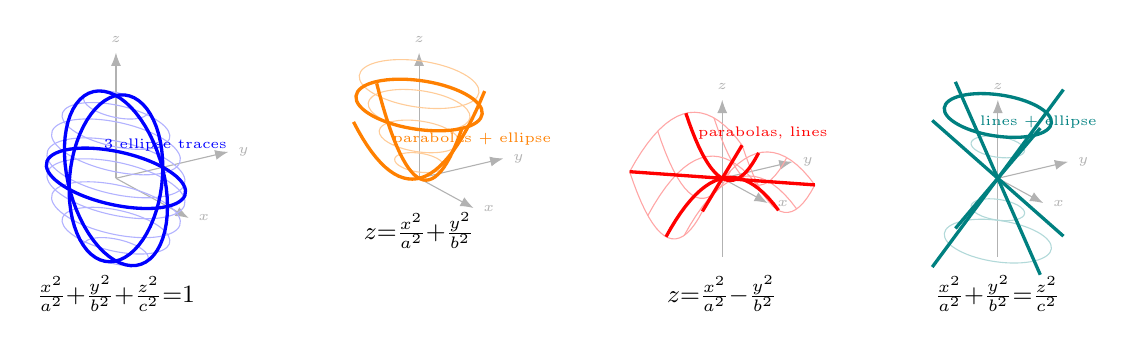
\begin{tikzpicture}[>=Latex,scale=0.7,x={(0.55cm,-0.3cm)},y={(0.85cm,0.2cm)},z={(0cm,0.95cm)}]
  % ellipsoid
  \begin{scope}
    \draw[->,gray!60] (0,0,0)--(2.4,0,0) node[right,font=\tiny]{$x$};
    \draw[->,gray!60] (0,0,0)--(0,2.4,0) node[right,font=\tiny]{$y$};
    \draw[->,gray!60] (0,0,0)--(0,0,2.4) node[above,font=\tiny]{$z$};
    \foreach \z in {-1.4,-1.0,...,1.4} {
      \pgfmathsetmacro{\rr}{sqrt(max(0,1-\z*\z/2.5))}
      \draw[blue!30] (0,0,\z) ellipse ({1.7*\rr} and {1.0*\rr});
    }
    % traces: bold ellipses in each coord plane
    \draw[blue,very thick] (0,0,0) ellipse (1.7 and 1.0);
    \draw[blue,very thick,domain=0:360,samples=60,variable=\t] plot ({1.7*cos(\t)},0,{1.58*sin(\t)});
    \draw[blue,very thick,domain=0:360,samples=60,variable=\t] plot (0,{1.0*cos(\t)},{1.58*sin(\t)});
    \node at (0,0,-2.2){\small $\tfrac{x^2}{a^2}{+}\tfrac{y^2}{b^2}{+}\tfrac{z^2}{c^2}{=}1$};
    \node[blue,font=\tiny] at (2.4,-0.5,1.5){3 ellipse traces};
  \end{scope}
  % elliptic paraboloid
  \begin{scope}[xshift=5.5cm]
    \draw[->,gray!60] (0,0,0)--(1.8,0,0) node[right,font=\tiny]{$x$};
    \draw[->,gray!60] (0,0,0)--(0,1.8,0) node[right,font=\tiny]{$y$};
    \draw[->,gray!60] (0,0,0)--(0,0,2.4) node[above,font=\tiny]{$z$};
    \foreach \z in {0.3,0.8,1.3,1.8} {
      \pgfmathsetmacro{\rr}{sqrt(\z)}
      \draw[orange!40] (0,0,\z) ellipse ({\rr} and {0.7*\rr});
    }
    % traces: 2 parabolas + 1 ellipse
    \draw[orange,very thick,domain=-1.4:1.4,samples=30] plot (\x,0,{0.7*\x*\x});
    \draw[orange,very thick,domain=-1.4:1.4,samples=30] plot (0,\x,{0.7*\x*\x});
    \draw[orange,very thick] (0,0,1.4) ellipse ({sqrt(2.0)} and {0.7*sqrt(2.0)});
    \node at (0,0,-1){\small $z{=}\tfrac{x^2}{a^2}{+}\tfrac{y^2}{b^2}$};
    \node[orange,font=\tiny] at (2.2,-0.3,1.5){parabolas + ellipse};
  \end{scope}
  % saddle
  \begin{scope}[xshift=11cm]
    \draw[->,gray!60] (0,0,0)--(1.5,0,0) node[right,font=\tiny]{$x$};
    \draw[->,gray!60] (0,0,0)--(0,1.5,0) node[right,font=\tiny]{$y$};
    \draw[->,gray!60] (0,0,-1.5)--(0,0,1.5) node[above,font=\tiny]{$z$};
    \foreach \v in {-1.2,-0.6,0,0.6,1.2}
      \draw[red!35,thin,domain=-1.2:1.2,samples=20,variable=\u] plot (\u,\v,{0.6*(\u*\u-\v*\v)});
    \foreach \u in {-1.2,-0.6,0,0.6,1.2}
      \draw[red!35,thin,domain=-1.2:1.2,samples=20,variable=\v] plot (\u,\v,{0.6*(\u*\u-\v*\v)});
    % traces: parabola up in xz, parabola down in yz, 2 lines in xy
    \draw[red,very thick,domain=-1.2:1.2,samples=24] plot (\x,0,{0.6*\x*\x});
    \draw[red,very thick,domain=-1.2:1.2,samples=24] plot (0,\x,{-0.6*\x*\x});
    \draw[red,very thick] (-1.2,-1.2,0)--(1.2,1.2,0);
    \draw[red,very thick] (-1.2,1.2,0)--(1.2,-1.2,0);
    \node at (0,0,-2.2){\small $z{=}\tfrac{x^2}{a^2}{-}\tfrac{y^2}{b^2}$};
    \node[red,font=\tiny] at (1.8,-0.3,1.5){parabolas, lines};
  \end{scope}
  % cone
  \begin{scope}[xshift=16cm]
    \draw[->,gray!60] (0,0,0)--(1.5,0,0) node[right,font=\tiny]{$x$};
    \draw[->,gray!60] (0,0,0)--(0,1.5,0) node[right,font=\tiny]{$y$};
    \draw[->,gray!60] (0,0,-1.5)--(0,0,1.5) node[above,font=\tiny]{$z$};
    \foreach \z in {-1.2,-0.6,0.6,1.2} \draw[teal!30] (0,0,\z) ellipse ({abs(\z)} and {0.7*abs(\z)});
    % traces: 4 lines (xz, yz planes) + ellipse at z=1
    \draw[teal,very thick] (-1.4,0,1.4)--(0,0,0)--(1.4,0,1.4);
    \draw[teal,very thick] (0,-1.4,1.4)--(0,0,0)--(0,1.4,1.4);
    \draw[teal,very thick] (-1.4,0,-1.4)--(0,0,0)--(1.4,0,-1.4);
    \draw[teal,very thick] (0,-1.4,-1.4)--(0,0,0)--(0,1.4,-1.4);
    \draw[teal,very thick] (0,0,1.2) ellipse (1.2 and {0.7*1.2});
    \node at (0,0,-2.2){\small $\tfrac{x^2}{a^2}{+}\tfrac{y^2}{b^2}{=}\tfrac{z^2}{c^2}$};
    \node[teal,font=\tiny] at (1.8,-0.3,1.7){lines + ellipse};
  \end{scope}
\end{tikzpicture}

\medskip

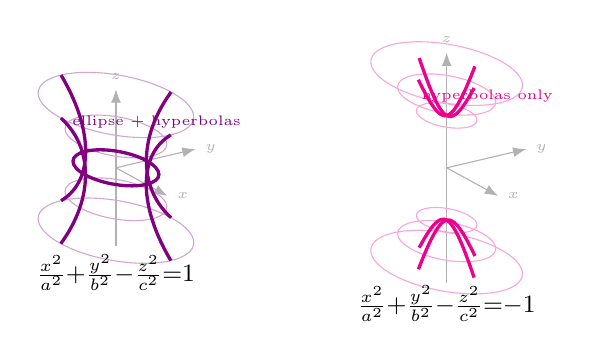
\begin{tikzpicture}[>=Latex,scale=0.7,x={(0.55cm,-0.3cm)},y={(0.85cm,0.2cm)},z={(0cm,0.95cm)}]
  % hyperboloid one sheet
  \begin{scope}
    \draw[->,gray!60] (0,0,0)--(1.7,0,0) node[right,font=\tiny]{$x$};
    \draw[->,gray!60] (0,0,0)--(0,1.7,0) node[right,font=\tiny]{$y$};
    \draw[->,gray!60] (0,0,-1.5)--(0,0,1.5) node[above,font=\tiny]{$z$};
    \foreach \z in {-1.2,-0.6,0,0.6,1.2} {
      \pgfmathsetmacro{\rr}{cosh(\z)}
      \draw[violet!35] (0,0,\z) ellipse ({\rr} and {0.65*\rr});
    }
    % traces: ellipse at z=0 + hyperbolas in xz,yz
    \draw[violet,very thick] (0,0,0) ellipse (1.0 and 0.65);
    \draw[violet,very thick,domain=-1.2:1.2,samples=30] plot ({cosh(\x)},0,\x);
    \draw[violet,very thick,domain=-1.2:1.2,samples=30] plot ({-cosh(\x)},0,\x);
    \draw[violet,very thick,domain=-1.2:1.2,samples=30] plot (0,{0.65*cosh(\x)},\x);
    \draw[violet,very thick,domain=-1.2:1.2,samples=30] plot (0,{-0.65*cosh(\x)},\x);
    \node at (0,0,-2){\small $\tfrac{x^2}{a^2}{+}\tfrac{y^2}{b^2}{-}\tfrac{z^2}{c^2}{=}1$};
    \node[violet,font=\tiny] at (1.8,-0.3,1.5){ellipse + hyperbolas};
  \end{scope}
  % hyperboloid two sheets
  \begin{scope}[xshift=6cm]
    \draw[->,gray!60] (0,0,0)--(1.7,0,0) node[right,font=\tiny]{$x$};
    \draw[->,gray!60] (0,0,0)--(0,1.7,0) node[right,font=\tiny]{$y$};
    \draw[->,gray!60] (0,0,-2.2)--(0,0,2.2) node[above,font=\tiny]{$z$};
    \foreach \z in {1.0,1.4,1.8,-1.0,-1.4,-1.8} {
      \pgfmathsetmacro{\rr}{0.6*sinh(abs(\z))}
      \draw[magenta!35] (0,0,\z) ellipse ({\rr} and {0.65*\rr});
    }
    % traces: hyperbolas in xz, yz (no real ellipse near origin)
    \draw[magenta,very thick,domain=0:1.2,samples=22] plot ({0.6*sinh(\x)},0,{cosh(\x)});
    \draw[magenta,very thick,domain=0:1.2,samples=22] plot ({-0.6*sinh(\x)},0,{cosh(\x)});
    \draw[magenta,very thick,domain=0:1.2,samples=22] plot ({0.6*sinh(\x)},0,{-cosh(\x)});
    \draw[magenta,very thick,domain=0:1.2,samples=22] plot ({-0.6*sinh(\x)},0,{-cosh(\x)});
    \draw[magenta,very thick,domain=0:1.2,samples=22] plot (0,{0.4*sinh(\x)},{cosh(\x)});
    \draw[magenta,very thick,domain=0:1.2,samples=22] plot (0,{-0.4*sinh(\x)},{cosh(\x)});
    \draw[magenta,very thick,domain=0:1.2,samples=22] plot (0,{0.4*sinh(\x)},{-cosh(\x)});
    \draw[magenta,very thick,domain=0:1.2,samples=22] plot (0,{-0.4*sinh(\x)},{-cosh(\x)});
    \node at (0,0,-2.6){\small $\tfrac{x^2}{a^2}{+}\tfrac{y^2}{b^2}{-}\tfrac{z^2}{c^2}{=}{-}1$};
    \node[magenta,font=\tiny] at (1.8,-0.3,2.0){hyperbolas only};
  \end{scope}
\end{tikzpicture}
\end{center}

\newpage
%                       --
\section{Chapter 13: Vector Functions}
%                       --

\subsection{13.1 Vector Functions and Space Curves}

\textbf{Limits and continuity.} $\lim_{t\to a}\vec{r}(t)=\vv{\lim f,\lim g,\lim h}$ component-wise; $\vec{r}$ continuous iff each component continuous.

$\vec{r}(t) = \vv{f(t),g(t),h(t)}$; operations (addition, scaling, dot, cross) are component-wise.

\textbf{Direction of traversal.} Arrowheads show direction as $t$ increases. Reversing the parameter reverses the arrow.

\begin{center}
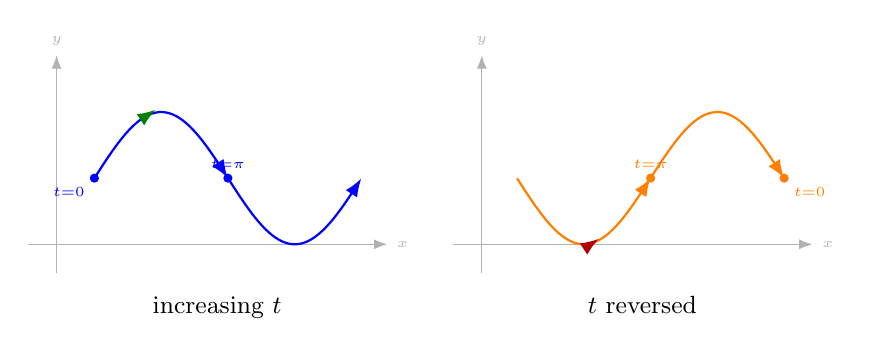
\begin{tikzpicture}[>=Latex,scale=1.2]
  \begin{scope}
    \draw[->,gray!60] (-0.3,0)--(3.5,0) node[right,font=\tiny]{$x$};
    \draw[->,gray!60] (0,-0.3)--(0,2.0) node[above,font=\tiny]{$y$};
    \draw[thick,blue,->,domain=0:3.14,samples=40] plot ({0.4+0.45*\x},{0.7+0.7*sin(\x r)});
    \draw[thick,blue,->,domain=3.14:6.28,samples=40] plot ({0.4+0.45*\x},{0.7+0.7*sin(\x r)});
    \filldraw[blue] (0.4,0.7) circle (1.2pt) node[below left,font=\tiny]{$t{=}0$};
    \filldraw[blue] ({0.4+0.45*3.14},0.7) circle (1.2pt) node[above,font=\tiny]{$t{=}\pi$};
    \draw[->,green!50!black,thick] ({0.4+0.45*1.2},{0.7+0.7*sin(1.2 r)}) -- ({0.4+0.45*1.2+0.3*cos(1.2 r)},{0.7+0.7*sin(1.2 r)+0.2*cos(1.2 r)});
    \node[below,font=\small] at (1.7,-0.45){increasing $t$};
  \end{scope}
  \begin{scope}[xshift=4.5cm]
    \draw[->,gray!60] (-0.3,0)--(3.5,0) node[right,font=\tiny]{$x$};
    \draw[->,gray!60] (0,-0.3)--(0,2.0) node[above,font=\tiny]{$y$};
    \draw[thick,orange,->,domain=6.28:3.14,samples=40] plot ({3.2-0.45*\x},{0.7+0.7*sin(\x r)});
    \draw[thick,orange,->,domain=3.14:0,samples=40] plot ({3.2-0.45*\x},{0.7+0.7*sin(\x r)});
    \filldraw[orange] (3.2,0.7) circle (1.2pt) node[below right,font=\tiny]{$t{=}0$};
    \filldraw[orange] ({3.2-0.45*3.14},0.7) circle (1.2pt) node[above,font=\tiny]{$t{=}\pi$};
    \draw[->,red!70!black,thick] ({3.2-0.45*4.5},{0.7+0.7*sin(4.5 r)}) -- ({3.2-0.45*4.5-0.3*cos(4.5 r)},{0.7+0.7*sin(4.5 r)-0.2*cos(4.5 r)});
    \node[below,font=\small] at (1.7,-0.45){$t$ reversed};
  \end{scope}
\end{tikzpicture}
\end{center}

\medskip\textbf{Practice.}
\begin{enumerate}[noitemsep]
  \item Sketch the directed curve $\vec{r}(t)=\langle 3\cos t, 3\sin t, 2\rangle$ for $0\le t\le 2\pi$. Indicate the direction of motion.
  \item Sketch the curve $\vec{r}(t)=\langle t^2, t\rangle$ in 2D and describe its shape.
  \item Find the domain of $\vec{r}(t)=\langle \ln(t-1),\; \arctan(t),\; \sqrt{4-t^2}\rangle$.
\end{enumerate}

\begin{center}
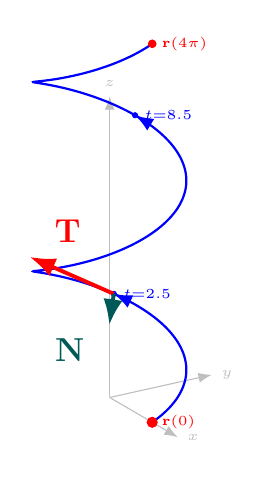
\begin{tikzpicture}[>=Latex,scale=0.9,x={(0.6cm,-0.35cm)},y={(0.9cm,0.2cm)},z={(0cm,0.85cm)}]
  \draw[->,gray!50,thin] (0,0,0) -- (1.6,0,0) node[right,font=\tiny]{$x$};
  \draw[->,gray!50,thin] (0,0,0) -- (0,1.6,0) node[right,font=\tiny]{$y$};
  \draw[->,gray!50,thin] (0,0,0) -- (0,0,5) node[above,font=\tiny]{$z$};
  % Helix r(t) = (cos t, sin t, t/2) for t in [0, 4pi]
  \draw[thick,blue,domain=0:4*pi,samples=160,variable=\t,smooth]
    plot ({cos(\t r)},{sin(\t r)},{\t/2});
  % Mark start and end
  \filldraw[red] (1,0,0) circle (2pt) node[right,red,font=\tiny]{$\vec r(0)$};
  \filldraw[red] ({cos(4*pi r)},{sin(4*pi r)},{2*pi}) circle (1.5pt) node[right,red,font=\tiny]{$\vec r(4\pi)$};
  % Two arrowheads on helix to indicate direction
  \pgfmathsetmacro{\ta}{2.5}
  \draw[->,blue,thick] ({cos((\ta-0.1) r)},{sin((\ta-0.1) r)},{(\ta-0.1)/2})
                    -- ({cos(\ta r)},{sin(\ta r)},{\ta/2});
  \pgfmathsetmacro{\tb}{8.5}
  \draw[->,blue,thick] ({cos((\tb-0.1) r)},{sin((\tb-0.1) r)},{(\tb-0.1)/2})
                    -- ({cos(\tb r)},{sin(\tb r)},{\tb/2});
  \filldraw[blue] ({cos(\ta r)},{sin(\ta r)},{\ta/2}) circle (1pt) node[right,font=\tiny]{$t{=}2.5$};
  \filldraw[blue] ({cos(\tb r)},{sin(\tb r)},{\tb/2}) circle (1pt) node[right,font=\tiny]{$t{=}8.5$};
  % TNB frame at t=2.5
  \pgfmathsetmacro{\Tx}{-sin(\ta r)}\pgfmathsetmacro{\Ty}{cos(\ta r)}\pgfmathsetmacro{\Tz}{0.5}
  \pgfmathsetmacro{\Nx}{-cos(\ta r)}\pgfmathsetmacro{\Ny}{-sin(\ta r)}
  \pgfmathsetmacro{\nrmB}{sqrt(1.25)}\pgfmathsetmacro{\Bx}{(cos(\ta r)*0.5+sin(\ta r))/\nrmB}\pgfmathsetmacro{\By}{(sin(\ta r)*0.5-cos(\ta r))/\nrmB}
  \draw[->,red,line width=1.4pt] ({cos(\ta r)},{sin(\ta r)},{\ta/2})--({cos(\ta r)+1.1*\Tx},{sin(\ta r)+1.1*\Ty},{\ta/2+1.1*\Tz}) node[above right=1pt,red,font=\large\bfseries,xshift=4pt]{$\vec T$};
  \draw[->,teal!70!black,line width=1.4pt] ({cos(\ta r)},{sin(\ta r)},{\ta/2})--({cos(\ta r)+1.1*\Nx},{sin(\ta r)+1.1*\Ny},{\ta/2}) node[below left=1pt,teal!70!black,font=\large\bfseries,xshift=-4pt]{$\vec N$};
\end{tikzpicture}
\end{center}

\textit{2D projections.} the $xy$-shadow is a circle (the first two components). the $z$-component grows linearly with $t$.

\begin{center}
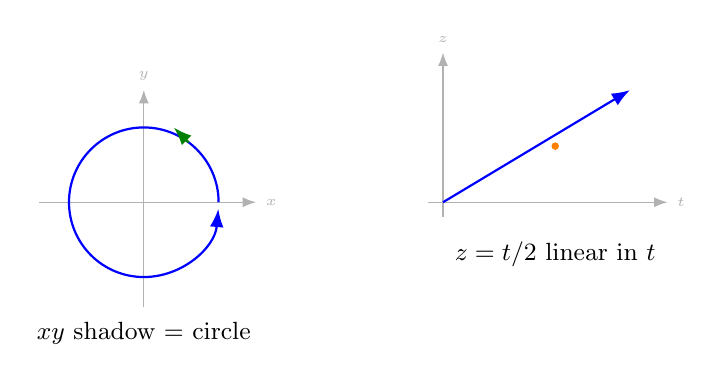
\begin{tikzpicture}[>=Latex,scale=0.95]
  % xy projection
  \begin{scope}
    \draw[->,gray!60] (-1.4,0)--(1.5,0) node[right,font=\tiny]{$x$};
    \draw[->,gray!60] (0,-1.4)--(0,1.5) node[above,font=\tiny]{$y$};
    \draw[thick,blue,->] (1,0) arc (0:355:1);
    \draw[->,green!50!black,thick] (0.6,0.8) -- (0.4,1.0);
    \node[font=\small] at (0,-1.75){$xy$ shadow $=$ circle};
  \end{scope}
  % z vs t plot
  \begin{scope}[xshift=4cm]
    \draw[->,gray!60] (-0.2,0)--(3,0) node[right,font=\tiny]{$t$};
    \draw[->,gray!60] (0,-0.2)--(0,2) node[above,font=\tiny]{$z$};
    \draw[thick,blue,->] (0,0)--(2.5,1.5);
    \filldraw[orange] (1.5,0.75) circle (1.2pt);
    \node[font=\small] at (1.5,-0.7){$z=t/2$ linear in $t$};
  \end{scope}
\end{tikzpicture}
\end{center}

\subsection{13.2 Derivatives and Integrals of Vector Functions}

\textbf{Derivative.}
\[
\vec{r}'(t) = \lim_{h\to 0}\frac{\vec{r}(t+h)-\vec{r}(t)}{h} = \vv{f'(t),g'(t),h'(t)}
\]
Geometrically, the tangent vector points in direction of motion.

\textbf{Unit tangent vector.} $\vec{T}(t) = \dfrac{\vec{r}'(t)}{|\vec{r}'(t)|}$

\textbf{Differentiation rules} (same form as scalar):
\begin{itemize}[noitemsep]
\item $(\vec{u}\cdot\vec{v})' = \vec{u}'\cdot\vec{v}+\vec{u}\cdot\vec{v}'$
\item $(\vec{u}\times\vec{v})' = \vec{u}'\times\vec{v}+\vec{u}\times\vec{v}'$
\end{itemize}

\begin{thm}
$|\vec{r}(t)|=c$ (constant) $\implies \vec{r}'(t)\perp\vec{r}(t)$.
\end{thm}
\textit{Proof.} Differentiate $\vec{r}\cdot\vec{r}=c^2$: $2\vec{r}'\cdot\vec{r}=0$ $\implies$ $\vec{r}'\perp\vec{r}$.

\textbf{Integral.} $\int_a^b \vec{r}(t)\,dt = \vv{\int_a^b f\,dt,\;\int_a^b g\,dt,\;\int_a^b h\,dt}$

\medskip\textbf{Practice.}
\begin{enumerate}[noitemsep]
  \item Given $\vec{r}(t)=\langle t^2,\sin t,e^t\rangle$, find the velocity $\vec{v}(t)$ and acceleration $\vec{a}(t)$ at $t=0$.
  \item If a particle moves with constant speed, show that its velocity and acceleration vectors are always orthogonal.
\end{enumerate}

\subsection{13.3 Arc Length and Curvature}

\textbf{Arc length.} Small arc element: $ds\approx |\vec{r}'(t)|\,dt$ (Pythagorean theorem).
\[
L = \int_a^b |\vec{r}'(t)|\,dt = \int_a^b \sqrt{(x')^2+(y')^2+(z')^2}\,dt
\]

\textbf{Arc length function.} $s(t)=\int_a^t |\vec{r}'(u)|\,du$; \quad $ds/dt=|\vec{r}'(t)|$ (speed).

\textbf{Curvature.}
\[
\kappa = \left|\frac{d\vec{T}}{ds}\right| = \frac{|\vec{T}'(t)|}{|\vec{r}'(t)|} = \frac{|\vec{r}'(t)\times\vec{r}''(t)|}{|\vec{r}'(t)|^3}
\]
For $y=f(x)$: $\kappa = \dfrac{|f''|}{(1+(f')^2)^{3/2}}$

\textbf{Principal unit normal.} $\vec{N}(t) = \dfrac{\vec{T}'(t)}{|\vec{T}'(t)|}$ (points toward center of curvature).

\textbf{Radius of curvature.} $\rho = 1/\kappa$; the \emph{osculating circle} has radius $\rho$ and center in the direction of $\vec{N}$.

\begin{center}
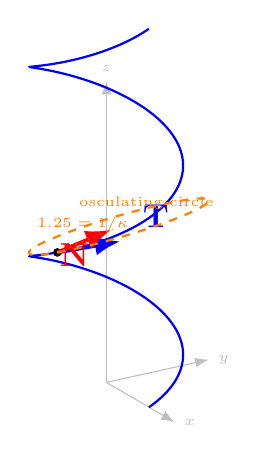
\begin{tikzpicture}[>=Latex,scale=0.9,x={(0.6cm,-0.35cm)},y={(0.9cm,0.2cm)},z={(0cm,0.85cm)}]
  \draw[->,gray!50,thin] (0,0,0) -- (1.6,0,0) node[right,font=\tiny]{$x$};
  \draw[->,gray!50,thin] (0,0,0) -- (0,1.6,0) node[right,font=\tiny]{$y$};
  \draw[->,gray!50,thin] (0,0,0) -- (0,0,5) node[above,font=\tiny]{$z$};
  % Reuse the same helix from 13.1: r(t) = (cos t, sin t, t/2), t in [0, 4 pi]
  \draw[thick,blue,domain=0:4*pi,samples=160,variable=\t,smooth]
    plot ({cos(\t r)},{sin(\t r)},{\t/2});
  % Sample point at t = 5 (radians)
  \pgfmathsetmacro{\ts}{5.0}
  \pgfmathsetmacro{\cs}{cos(\ts r)}
  \pgfmathsetmacro{\ss}{sin(\ts r)}
  \pgfmathsetmacro{\zs}{\ts/2}
  \filldraw[black] ({\cs},{\ss},{\zs}) circle (1.5pt);
  % Unit tangent T = (-sin t, cos t, 1/2) / |...|; |...| = sqrt(1.25)
  \pgfmathsetmacro{\nrm}{sqrt(1.25)}
  \draw[->,blue,line width=1.4pt] ({\cs},{\ss},{\zs})
                    -- ({\cs+1.2*(-\ss)/\nrm},{\ss+1.2*\cs/\nrm},{\zs+1.2*0.5/\nrm})
    node[above right=1pt,blue,font=\large\bfseries,xshift=3pt]{$\vec T$};
  % Principal normal N = (-cos t, -sin t, 0) (radially inward on a helix)
  \draw[->,red,line width=1.4pt] ({\cs},{\ss},{\zs}) -- ({\cs-1.1*\cs},{\ss-1.1*\ss},{\zs})
    node[below left=1pt,red,font=\large\bfseries,xshift=-3pt]{$\vec N$};
  % Osculating circle of radius rho = 1.25 IN THE T-N PLANE
  % center = sample + rho * N_hat, where N_hat = (-cs, -ss, 0)
  % T_hat = (-ss, cs, 0.5)/sqrt(1.25)
  % Circle: P(s) = center + rho*(-cos(s)*N_hat + sin(s)*T_hat)
  \pgfmathsetmacro{\rho}{1.25}
  \pgfmathsetmacro{\Cx}{\cs-\rho*\cs}
  \pgfmathsetmacro{\Cy}{\ss-\rho*\ss}
  \pgfmathsetmacro{\Cz}{\zs}
  \pgfmathsetmacro{\Txn}{(-\ss)/\nrm}
  \pgfmathsetmacro{\Tyn}{\cs/\nrm}
  \pgfmathsetmacro{\Tzn}{0.5/\nrm}
  \draw[dashed,orange,thick,domain=0:360,samples=80,variable=\s]
    plot ({\Cx + \rho*cos(\s)*(-(-\cs)) + \rho*sin(\s)*\Txn},
          {\Cy + \rho*cos(\s)*(-(-\ss)) + \rho*sin(\s)*\Tyn},
          {\Cz + \rho*cos(\s)*0          + \rho*sin(\s)*\Tzn});
  \draw[dotted,orange] ({\cs},{\ss},{\zs}) -- ({\Cx},{\Cy},{\Cz});
  \node[orange,font=\tiny] at ({\Cx+0.2},{\Cy+0.3},{\Cz+0.4}){osculating circle};
  \node[orange,font=\tiny] at ({\cs-0.15},{\ss+0.5},{\zs+0.3}){$\rho=1/\kappa$};
\end{tikzpicture}
\end{center}

\medskip\textbf{Practice.}
\begin{enumerate}[noitemsep]
  \item Find the length of the arc of the helix $\vec{r}(t)=\langle\cos t,\sin t,t\rangle$ from $t=0$ to $t=2\pi$.
  \item Find the curvature of the parabola $y=x^2$ at the origin.
  \item Find the unit tangent vector $\vec{T}(t)$ and unit normal $\vec{N}(t)$ for the helix $\vec{r}(t)=\langle\cos t,\sin t,t\rangle$.
\end{enumerate}

\subsection{13.4 Motion in Space: Velocity and Acceleration}

\textbf{Velocity, speed, acceleration.}
\[
\vec{v}(t)=\vec{r}'(t),\quad \text{speed}=|\vec{v}(t)|=\frac{ds}{dt},\quad \vec{a}(t)=\vec{v}'(t)=\vec{r}''(t)
\]

\textbf{Tangential/normal decomposition.}
\[
\vec{a} = a_T\vec{T}+a_N\vec{N}, \qquad a_T = \frac{d|\vec{v}|}{dt} = \frac{\vec{r}'\cdot\vec{r}''}{|\vec{r}'|}, \qquad a_N = \kappa|\vec{v}|^2 = \frac{|\vec{r}'\times\vec{r}''|}{|\vec{r}'|}
\]

\textit{$a_T$ is the speeding-up/slowing-down part, $a_N$ is the turning (centripetal) part.}

\begin{center}
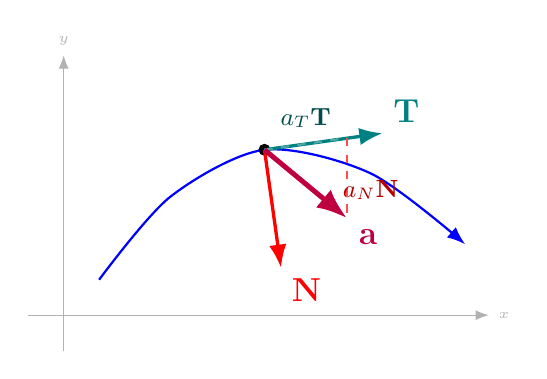
\begin{tikzpicture}[>=Latex,scale=1.5]
  % Curve
  \draw[->,gray!60] (-0.3,0)--(3.6,0) node[right,font=\tiny]{$x$};
  \draw[->,gray!60] (0,-0.3)--(0,2.2) node[above,font=\tiny]{$y$};
  \draw[thick,blue,->,smooth] plot coordinates {(0.3,0.3)(0.9,1.0)(1.7,1.4)(2.6,1.2)(3.4,0.6)};
  % Sample point
  \coordinate (P) at (1.7,1.4);
  \filldraw[black] (P) circle (1.3pt);
  % Tangent direction T (along curve direction)
  \draw[->,teal,line width=1.2pt] (P)--++(1.0,0.14) node[above right,font=\large\bfseries,teal]{T};
  % Normal N (perpendicular, toward concavity / inside of curve)
  \draw[->,red,line width=1.2pt] (P)--++(0.14,-1.0) node[below right,font=\large\bfseries,red]{N};
  % Dashed component legs (no yellow fill)
  \draw[teal!70,dashed,thick] (P)--++(0.7,0.1);
  \draw[red!70,dashed,thick] ($(P)+(0.7,0.1)$)--++(0.0,-0.68);
  % Acceleration vector (purple) — hypotenuse
  \draw[->,purple,line width=1.8pt] (P)--++(0.7,-0.58) node[below right,font=\large\bfseries,purple]{a};
  % Component labels along the legs
  \node[teal!60!black,font=\small] at ({1.7+0.35},{1.4+0.27}){$a_T\vec T$};
  \node[red!70!black,font=\small] at ({1.7+0.9},{1.4-0.34}){$a_N\vec N$};
\end{tikzpicture}
\end{center}

\textbf{Projectile motion.} $\vec{a}=-g\jhat$. integrate twice with initial $\vec r(0)$ and $\vec v(0)$.

\textit{Example.} fire from origin with $\vec v(0)=(v_0\cos\alpha)\ihat+(v_0\sin\alpha)\jhat$. then $\vec v(t)=\vv{v_0\cos\alpha,\;v_0\sin\alpha-gt}$ and $\vec r(t)=\vv{v_0\cos\alpha\cdot t,\;v_0\sin\alpha\cdot t-\tfrac{g}{2}t^2}$. range $=v_0^2\sin 2\alpha/g$.

\begin{center}
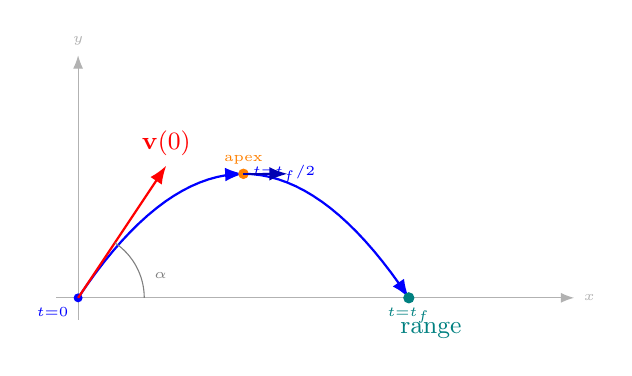
\begin{tikzpicture}[>=Latex,scale=1.4]
  \draw[->,gray!60] (-0.2,0)--(4.5,0) node[right,font=\tiny]{$x$};
  \draw[->,gray!60] (0,-0.2)--(0,2.2) node[above,font=\tiny]{$y$};
  % parabolic trajectory v0=5, alpha=60deg -> vx0=2.5, vy0=4.33; flight time = 2*vy0/g = 0.88, range = vx0*flight time = 2.21
  % Use simple v0cosa=2, v0sina=3, g=2 -> flight=3, range=6 too big. Use g=4 -> flight=1.5, range=3
  \pgfmathsetmacro{\vx}{2}\pgfmathsetmacro{\vy}{3}\pgfmathsetmacro{\g}{4}
  \pgfmathsetmacro{\tf}{2*\vy/\g}
  \pgfmathsetmacro{\thalf}{\tf/2}
  \draw[thick,blue,->,domain=0:\thalf,samples=20] plot ({\vx*\x},{\vy*\x-\g*\x*\x/2});
  \draw[thick,blue,->,domain=\thalf:\tf,samples=20] plot ({\vx*\x},{\vy*\x-\g*\x*\x/2});
  \filldraw[blue] (0,0) circle (1pt) node[below left,font=\tiny]{$t{=}0$};
  \filldraw[blue] ({\vx*\thalf},{\vy*\thalf-\g*\thalf*\thalf/2}) circle (1pt) node[right,font=\tiny]{$t{=}t_f/2$};
  % Initial velocity
  \draw[->,red,thick] (0,0)--({\vx*0.4},{\vy*0.4}) node[above,red,font=\small]{$\vec v(0)$};
  \draw[gray] (0.6,0) arc (0:{atan2(\vy,\vx)}:0.6);
  \node[gray,font=\tiny] at (0.75,0.2){$\alpha$};
  % Apex
  \pgfmathsetmacro{\ta}{\vy/\g}
  \pgfmathsetmacro{\xa}{\vx*\ta}
  \pgfmathsetmacro{\ya}{\vy*\ta-\g*\ta*\ta/2}
  \filldraw[orange] (\xa,\ya) circle (1.2pt) node[above,orange,font=\tiny]{apex};
  \draw[->,blue!70!black,thick] (\xa,\ya) -- ({\xa+0.4},{{\ya}});
  % Landing
  \pgfmathsetmacro{\xR}{\vx*\tf}
  \filldraw[teal] (\xR,0) circle (1.3pt) node[below,teal,font=\tiny]{$t{=}t_f$};
  \node[teal,font=\small] at ({\xR+0.2},-0.3){range};
\end{tikzpicture}
\end{center}

\medskip\textbf{Practice.}
\begin{enumerate}[noitemsep]
  \item Find the tangential and normal components of acceleration for $\vec{r}(t)=\langle t,t^2,3t\rangle$.
  \item A projectile is fired with initial speed $500\,\text{m/s}$ at angle $30^\circ$. Find range.
\end{enumerate}

\subsection{13.5 Taylor Approximation of Space Curves}

\textbf{Derivation.} Apply scalar Taylor expansion componentwise. Since $\vec{r}(t)=\vv{f(t),g(t),h(t)}$, each component satisfies $f(t_0+\delta)=f(t_0)+\delta f'(t_0)+\frac{\delta^2}{2}f''(t_0)+\cdots$ Similarly for $g$ and $h$, so:
\[
\vec{r}(t_0+h) = \vec{r}(t_0) + h\vec{r}'(t_0) + \frac{h^2}{2}\vec{r}''(t_0) + \frac{h^3}{6}\vec{r}'''(t_0) + \cdots
\]

\textbf{Geometric meaning.} Linear truncation gives tangent line. Quadratic adds osculating parabola. Cubic hugs curve even closer.

\textit{Example.} Take $\vec r(t)=(t,\;t^2/2,\;t^3/6)$, a true 3D curve.

\begin{center}
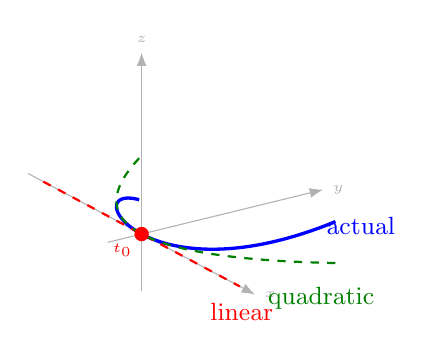
\begin{tikzpicture}[>=Latex,scale=1.6,x={(0.6cm,-0.32cm)},y={(0.9cm,0.22cm)},z={(0cm,0.9cm)}]
  \draw[->,gray!60] (-1.5,0,0)--(1.5,0,0) node[right,font=\tiny]{$x$};
  \draw[->,gray!60] (0,-0.3,0)--(0,1.6,0) node[right,font=\tiny]{$y$};
  \draw[->,gray!60] (0,0,-0.5)--(0,0,1.6) node[above,font=\tiny]{$z$};
  % Full 3D curve r(t) = (t, t^2/2, t^3/6)
  \draw[very thick,blue,domain=-1.3:1.3,samples=80,variable=\t,smooth]
    plot (\t,{0.5*\t*\t},{(1/6)*\t*\t*\t});
  % Linear approx: r(0)+t*(1,0,0)=(t,0,0): straight along x-axis
  \draw[red,thick,dashed,domain=-1.3:1.3,samples=20,variable=\t]
    plot (\t,0,0);
  % Quadratic: (t,t^2/2,0): parabola in xy-plane
  \draw[green!50!black,thick,dashed,domain=-1.3:1.3,samples=40,variable=\t]
    plot (\t,{0.5*\t*\t},0);
  % Base point at t=0
  \filldraw[red] (0,0,0) circle (1.5pt) node[below left,font=\tiny,red]{$t_0$};
  % Three clean labels
  \node[blue,font=\small] at (1.55,0.9,0.4){actual};
  \node[green!50!black,font=\small] at (1.55,0.55,-0.15){quadratic};
  \node[red,font=\small] at (1.55,-0.15,-0.1){linear};
\end{tikzpicture}
\end{center}

\textit{Linear truncation: $x$-axis tangent. Quadratic: $xy$-plane parabola. Cubic: adds $z$ wiggle which equals full curve for this example.}

\newpage
%                       --
\section{Chapter 14: Partial Derivatives}
%                       --

\subsection{14.1 Functions of Several Variables}

\textbf{Function of two variables.} $f:D\subset\R^2\to\R$. graph is a surface $z=f(x,y)$.

\textbf{Level curves.} $f(x,y)=k$, the contour lines. varying $k$ gives a contour map.

\textbf{Function of three variables.} $f(x,y,z)$, level surfaces $f(x,y,z)=k$.

\textit{close contours mean steep, wide contours mean shallow.}

\medskip\textbf{calc 1 recap.} in 1 variable we graph $y=f(x)$ as a curve. here $z=f(x,y)$ is a surface in $\R^3$.

\begin{center}
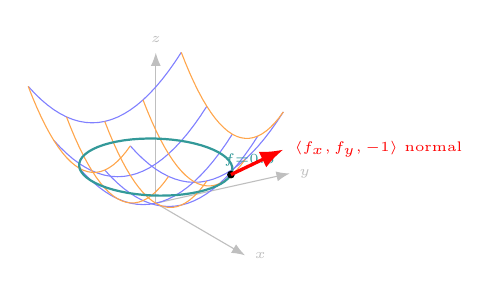
\begin{tikzpicture}[>=Latex,scale=0.9,x={(0.6cm,-0.35cm)},y={(0.9cm,0.2cm)},z={(0cm,0.85cm)}]
  % Left: 3D surface with xy-grid mapped on, axes labeled
  \draw[->,gray!50,thin] (0,0,0) -- (2.1,0,0) node[right,font=\tiny]{$x$};
  \draw[->,gray!50,thin] (0,0,0) -- (0,2.1,0) node[right,font=\tiny]{$y$};
  \draw[->,gray!50,thin] (0,0,0) -- (0,0,2.5) node[above,font=\tiny]{$z$};
  % Surface z = x^2 + y^2 (paraboloid) grid
  \foreach \u in {-1.2,-0.6,0,0.6,1.2}{
    \draw[blue!50,domain=-1.2:1.2,samples=25,variable=\v] plot (\u,\v,{0.6*(\u*\u+\v*\v)});
  }
  \foreach \v in {-1.2,-0.6,0,0.6,1.2}{
    \draw[orange!70,domain=-1.2:1.2,samples=25,variable=\u] plot (\u,\v,{0.6*(\u*\u+\v*\v)});
  }
  % Sample contour curve at z=0.6 (so x^2+y^2 = 1)
  \draw[teal!80,thick,domain=0:360,samples=60,variable=\t] plot ({cos(\t)},{sin(\t)},{0.6});
  \node[teal!80,font=\tiny] at ({0.4},{1.2},{0.6}){$f{=}0.6$};
  % Sample point on contour at angle 45
  \pgfmathsetmacro{\sa}{cos(45)}\pgfmathsetmacro{\sb}{sin(45)}
  \filldraw[black] (\sa,\sb,{0.6}) circle (1.3pt);
  % Outward normal in xy plane (which equals grad f direction up to z component)
  \draw[->,red,very thick] (\sa,\sb,{0.6})--({\sa+0.7*\sa},{\sb+0.7*\sb},{0.6+0.7*1.2*0.6}) node[right,red,font=\tiny]{$\langle f_x,f_y,-1\rangle$ normal};
\end{tikzpicture}
\qquad
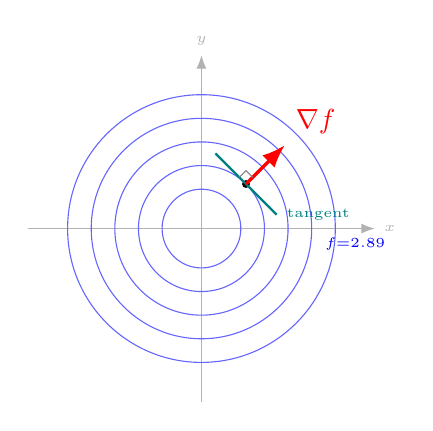
\begin{tikzpicture}[>=Latex,scale=1.0]
  % Right: contour map (top-down view) with clear perpendicularity
  \draw[->,gray!60] (-2.2,0)--(2.2,0) node[right,font=\tiny]{$x$};
  \draw[->,gray!60] (0,-2.2)--(0,2.2) node[above,font=\tiny]{$y$};
  \foreach \k in {0.25,0.64,1.21,1.96,2.89} {
    \pgfmathsetmacro{\r}{sqrt(\k)}
    \draw[blue!60] (0,0) circle (\r);
  }
  \node[blue,font=\tiny] at (1.95,-0.2){$f{=}2.89$};
  % Pick a point on a contour. Use the f=0.64 contour (radius 0.8), at angle 45 deg
  \pgfmathsetmacro{\rp}{0.8}
  \pgfmathsetmacro{\px}{\rp*cos(45)}
  \pgfmathsetmacro{\py}{\rp*sin(45)}
  \filldraw[black] (\px,\py) circle (1.2pt);
  % Tangent to contour at this point (perpendicular to radius)
  \draw[teal,thick] ({\px-0.55*sin(45)},{\py+0.55*cos(45)})
                 -- ({\px+0.55*sin(45)},{\py-0.55*cos(45)}) node[right,teal,font=\tiny]{tangent};
  % Gradient (radially outward at this point)
  \draw[->,red,very thick] (\px,\py) -- ({\px+0.7*cos(45)},{\py+0.7*sin(45)}) node[above right,red]{$\nabla f$};
  % Right angle marker
  \draw[gray] ({\px+0.12*cos(45)},{\py+0.12*sin(45)})
           -- ({\px+0.12*cos(45)+0.12*(-sin(45))},{\py+0.12*sin(45)+0.12*cos(45)})
           -- ({\px+0.12*(-sin(45))},{\py+0.12*cos(45)});
\end{tikzpicture}
\end{center}

\textit{Left.} surface $z=f(x,y)$ with grid lines mapped on. \textit{Right.} contour map of the same $f$; $\nabla f$ is always perpendicular to the contour through the point.

\begin{center}
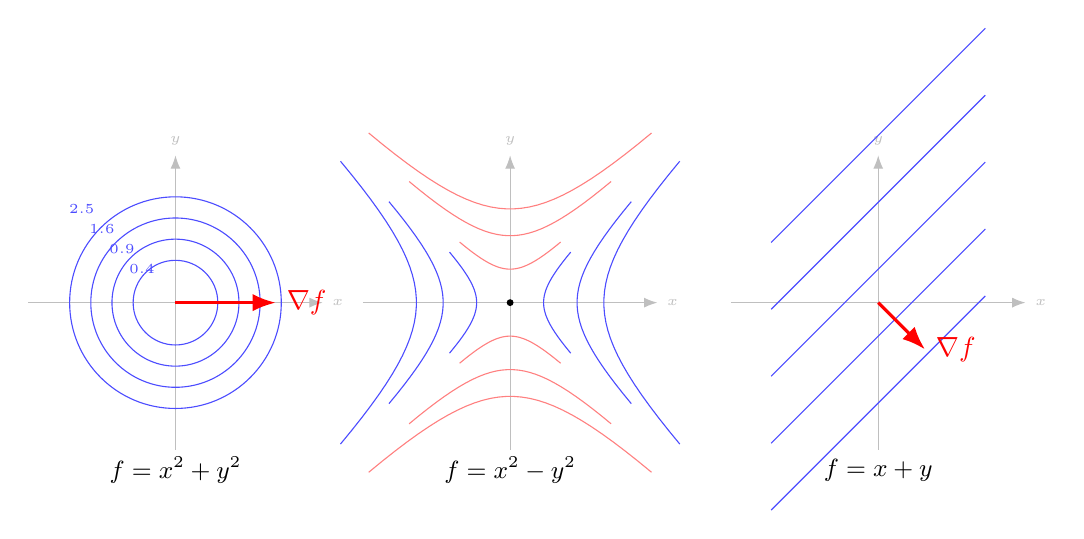
\begin{tikzpicture}[>=Latex,scale=0.85]
  % bowl: f = x^2+y^2 concentric circles with labels placed clear of curves
  \begin{scope}
    \draw[->,gray!50] (-2.2,0)--(2.2,0) node[right,font=\tiny]{$x$};
    \draw[->,gray!50] (0,-2.2)--(0,2.2) node[above,font=\tiny]{$y$};
    \foreach \k in {0.4, 0.9, 1.6, 2.5} {
      \pgfmathsetmacro{\r}{sqrt(\k)}
      \draw[blue!70] (0,0) circle (\r);
    }
    \node[blue!70,font=\tiny] at (-0.5,0.5){$0.4$};
    \node[blue!70,font=\tiny] at (-0.8,0.8){$0.9$};
    \node[blue!70,font=\tiny] at (-1.1,1.1){$1.6$};
    \node[blue!70,font=\tiny] at (-1.4,1.4){$2.5$};
    \draw[->,red,very thick] (0,0)--(1.5,0) node[right]{$\nabla f$};
    \node at (0,-2.5){\small $f=x^2+y^2$};
  \end{scope}
  % saddle
  \begin{scope}[xshift=5cm]
    \draw[->,gray!50] (-2.2,0)--(2.2,0) node[right,font=\tiny]{$x$};
    \draw[->,gray!50] (0,-2.2)--(0,2.2) node[above,font=\tiny]{$y$};
    \foreach \a in {0.5,1.0,1.4} {
      \draw[blue!70,domain=-1.2:1.2,samples=30] plot ({\a*cosh(\x)},{\a*sinh(\x)});
      \draw[blue!70,domain=-1.2:1.2,samples=30] plot ({-\a*cosh(\x)},{\a*sinh(\x)});
      \draw[red!50,domain=-1.2:1.2,samples=30] plot ({\a*sinh(\x)},{\a*cosh(\x)});
      \draw[red!50,domain=-1.2:1.2,samples=30] plot ({\a*sinh(\x)},{-\a*cosh(\x)});
    }
    \filldraw (0,0) circle (1.2pt);
    \node at (0,-2.5){\small $f=x^2-y^2$};
  \end{scope}
  % ridge / linear
  \begin{scope}[xshift=10.5cm]
    \draw[->,gray!50] (-2.2,0)--(2.2,0) node[right,font=\tiny]{$x$};
    \draw[->,gray!50] (0,-2.2)--(0,2.2) node[above,font=\tiny]{$y$};
    \foreach \k in {-1.5,-0.5,0.5,1.5,2.5} {
      \draw[blue!70] (-1.6,{\k-1.6})--(1.6,{\k+1.6});
    }
    \draw[->,red,very thick] (0,0)--(0.7,-0.7) node[right]{$\nabla f$};
    \node at (0,-2.5){\small $f=x+y$};
  \end{scope}
\end{tikzpicture}
\end{center}

\begin{center}
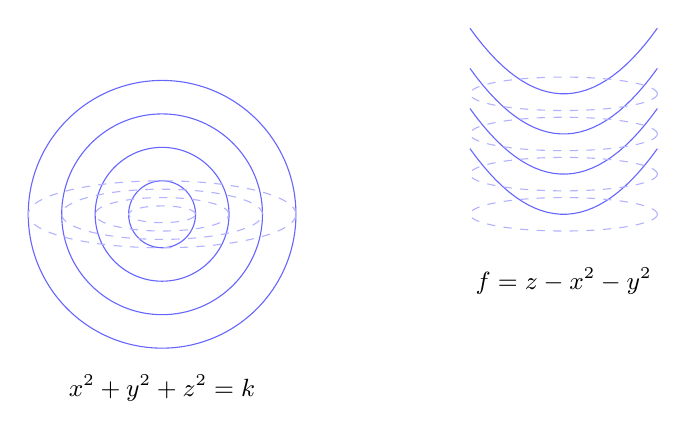
\begin{tikzpicture}[>=Latex,scale=0.85]
  % Nested spheres (cross-section view: nested circles, labeled as 3D)
  \begin{scope}
    \foreach \r/\rr in {0.5/0.125, 1.0/0.25, 1.5/0.375, 2.0/0.5} {
      \draw[blue!60] (0,0) circle (\r);
      \draw[blue!30,dashed] (0,0) ellipse ({\r} and {\rr});
    }
    \node at (0,-2.6){\small $x^2+y^2+z^2=k$};
  \end{scope}
  % Stacked paraboloids
  \begin{scope}[xshift=6cm]
    \foreach \k/\sh in {0/0, 0.5/0.6, 1.0/1.2, 1.5/1.8} {
      \draw[blue!60,domain=-1.4:1.4,samples=30] plot (\x,{0.5*\x*\x+\sh});
      \draw[blue!30,dashed] (0,\sh) ellipse (1.4 and 0.25);
    }
    \node at (0,-1){\small $f=z-x^2-y^2$};
  \end{scope}
\end{tikzpicture}
\end{center}

\medskip\textbf{Practice.}
\begin{enumerate}[noitemsep]
  \item Sketch the level curves of $f(x,y)=x^2+4y^2$ for $k=1,4,9$.
  \item Sketch the domain of $f(x,y)=\ln(y-x^2)$.
  \item Describe the level surfaces of $f(x,y,z)=x^2-y^2-z^2$ for $k>0$, $k=0$, and $k<0$.
\end{enumerate}

\subsection{14.2 Limits and Continuity}

\textbf{Limit.} $\lim_{(x,y)\to(a,b)}f(x,y)=L$ means $f\to L$ on \emph{every} path to $(a,b)$.

\textbf{DNE.} find two paths that disagree.

\textbf{Polar trick.} set $x=r\cos\theta,y=r\sin\theta$. if the value only depends on $r\to 0$ thats the limit.

\textbf{Continuity.} $f$ is continuous at $(a,b)$ if $\lim_{(x,y)\to(a,b)}f(x,y)=f(a,b)$. polynomials and rationals are continuous on their domains.

\textit{lines through origin.} for $f(x,y)=\dfrac{xy}{x^2+y^2}$ set $y=mx$. then $f=\dfrac{mx^2}{x^2+m^2x^2}=\dfrac{m}{1+m^2}$. value depends on $m$ so the limit doesnt exist.

\begin{center}
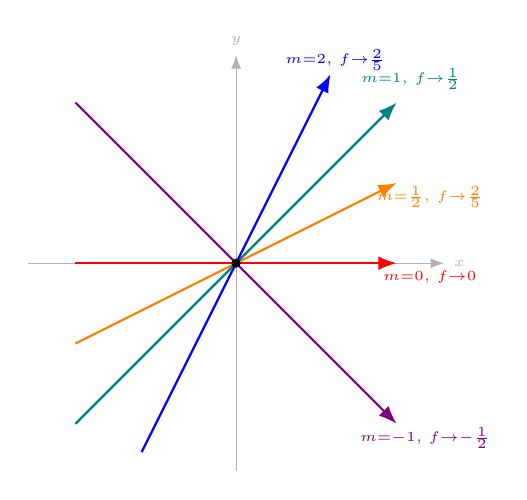
\begin{tikzpicture}[>=Latex,scale=1.2]
  \draw[->,gray!60] (-2.2,0)--(2.2,0) node[right,font=\tiny]{$x$};
  \draw[->,gray!60] (0,-2.2)--(0,2.2) node[above,font=\tiny]{$y$};
  \draw[->,red,thick] (-1.7,0)--(1.7,0);
  \node[red,font=\tiny] at (2.05,-0.15){$m{=}0,\,f{\to}0$};
  \draw[->,orange,thick] (-1.7,-0.85)--(1.7,0.85);
  \node[orange,font=\tiny] at (2.05,0.7){$m{=}\tfrac12,\,f{\to}\tfrac{2}{5}$};
  \draw[->,teal,thick] (-1.7,-1.7)--(1.7,1.7);
  \node[teal,font=\tiny] at (1.85,1.95){$m{=}1,\,f{\to}\tfrac12$};
  \draw[->,blue,thick] (-1.0,-2.0)--(1.0,2.0);
  \node[blue,font=\tiny] at (1.05,2.15){$m{=}2,\,f{\to}\tfrac{2}{5}$};
  \draw[->,violet,thick] (-1.7,1.7)--(1.7,-1.7);
  \node[violet,font=\tiny] at (2.0,-1.85){$m{=}{-1},\,f{\to}{-}\tfrac12$};
  \filldraw (0,0) circle (1.2pt);
\end{tikzpicture}
\end{center}

\textit{lines arent enough.} for $f(x,y)=\dfrac{xy^2}{x^2+y^4}$ every line $y=mx$ gives $f\to 0$. but along the parabola $x=y^2$ we get $f=\dfrac{y^4}{y^4+y^4}=\tfrac12$. so all lines agreeing is not enough for the limit to exist.

\begin{center}
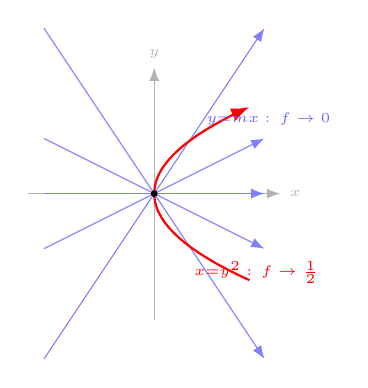
\begin{tikzpicture}[>=Latex,scale=1.0]
  \draw[->,gray!60] (-1.6,0)--(1.6,0) node[right,font=\tiny]{$x$};
  \draw[->,gray!60] (0,-1.6)--(0,1.6) node[above,font=\tiny]{$y$};
  \foreach \m in {-1.5,-0.5,0,0.5,1.5}{
    \draw[->,blue!50,thin] (-1.4,{\m*(-1.4)})--(1.4,{\m*1.4});
  }
  \draw[->,red,thick,domain=-1.1:1.1,samples=40] plot ({\x*\x},\x);
  \node[blue!60,font=\tiny] at (1.45,0.95){$y{=}mx:\,f\to 0$};
  \node[red,font=\tiny] at (1.3,-1.0){$x{=}y^2:\,f\to\tfrac12$};
  \filldraw (0,0) circle (1pt);
\end{tikzpicture}
\end{center}

\medskip\textbf{Practice.}
\begin{enumerate}[noitemsep]
  \item Evaluate the limit or show it does not exist: $\displaystyle\lim_{(x,y)\to(0,0)}\frac{x^2-y^2}{x^2+y^2}$.
  \item Use polar coordinates to evaluate $\displaystyle\lim_{(x,y)\to(0,0)}\frac{x^3+y^3}{x^2+y^2}$.
  \item Show that $\displaystyle\lim_{(x,y)\to(0,0)}\frac{xy^3}{x^2+y^6}$ does not exist, even though the limit is $0$ along every straight line through the origin.
\end{enumerate}

\subsection{14.3 Partial Derivatives}

\textbf{Definition.}
\[
f_x(x,y) = \lim_{h\to 0}\frac{f(x+h,y)-f(x,y)}{h} \qquad (\text{hold } y \text{ fixed})
\]
similarly $f_y$ holds $x$ fixed. notations $\partial f/\partial x$, $f_x$, $\partial z/\partial x$.

\medskip\textbf{calc 1 recap.} $f'(x)=\lim_{h\to0}[f(x+h)-f(x)]/h$. holding $y$ fixed makes $f$ depend on $x$ alone and you get the 1D derivative.

\textbf{Geometric.} $f_x$ is the slope of the trace cut by $y=$const, $f_y$ similar with $x=$const.

\begin{center}
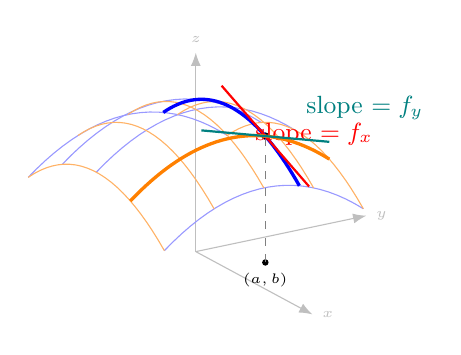
\begin{tikzpicture}[>=Latex,scale=0.95,x={(0.65cm,-0.35cm)},y={(0.95cm,0.2cm)},z={(0cm,0.95cm)}]
  \draw[->,gray!50] (0,0,0)--(2.4,0,0) node[right,font=\tiny]{$x$};
  \draw[->,gray!50] (0,0,0)--(0,2.4,0) node[right,font=\tiny]{$y$};
  \draw[->,gray!50] (0,0,0)--(0,0,2.8) node[above,font=\tiny]{$z$};
  % Surface z = 2 - 0.3(x^2+y^2) — gridded
  \foreach \u in {-1.4,-0.7,0,0.7,1.4}{
    \draw[blue!40,thin,domain=-1.4:1.4,samples=24,variable=\v] plot (\u,\v,{2-0.3*(\u*\u+\v*\v)});
  }
  \foreach \v in {-1.4,-0.7,0,0.7,1.4}{
    \draw[orange!60,thin,domain=-1.4:1.4,samples=24,variable=\u] plot (\u,\v,{2-0.3*(\u*\u+\v*\v)});
  }
  % Sample point (a,b) = (0.7, 0.5), value z = 2-0.3(0.49+0.25)=2-0.222=1.778
  \pgfmathsetmacro{\sa}{0.7} \pgfmathsetmacro{\sb}{0.5}
  \pgfmathsetmacro{\zv}{2-0.3*(\sa*\sa+\sb*\sb)}
  \filldraw[black] (\sa,\sb,\zv) circle (1.2pt);
  % Foot of point in xy plane
  \filldraw[black] (\sa,\sb,0) circle (1pt);
  \draw[dashed,gray] (\sa,\sb,0)--(\sa,\sb,\zv);
  % Trace y = sb (constant), highlighted blue
  \draw[blue,very thick,domain=-1.4:1.4,samples=40,variable=\v] plot (\v,\sb,{2-0.3*(\v*\v+\sb*\sb)});
  % Tangent in x direction at sample (slope = -0.6*sa = -0.42 in z per unit x)
  \pgfmathsetmacro{\mx}{-0.6*\sa}
  \draw[red,thick] ({\sa-0.9},\sb,{\zv-0.9*\mx}) -- ({\sa+0.9},\sb,{\zv+0.9*\mx});
  \node[red,font=\small] at (1.7,\sb,{\zv+0.4}){slope $=f_x$};
  % Trace x = sa (constant), highlighted orange
  \draw[orange,very thick,domain=-1.4:1.4,samples=40,variable=\v] plot (\sa,\v,{2-0.3*(\sa*\sa+\v*\v)});
  % Tangent in y direction at sample (slope = -0.6*sb = -0.3 in z per unit y)
  \pgfmathsetmacro{\my}{-0.6*\sb}
  \draw[teal,thick] (\sa,{\sb-0.9},{\zv-0.9*\my}) -- (\sa,{\sb+0.9},{\zv+0.9*\my});
  \node[teal,font=\small] at (\sa,1.9,{\zv+0.1}){slope $=f_y$};
  % Label the sample point
  \node[font=\tiny] at (\sa,\sb,-0.25){$(a,b)$};
\end{tikzpicture}
\end{center}

\textit{blue trace holds $y=b$, slope at $(a,b)$ is $f_x$. orange trace holds $x=a$, slope is $f_y$.}

\textbf{Higher partials.} $f_{xx}$, $f_{xy}=(f_x)_y$, $f_{yx}$, $f_{yy}$.

\begin{thm}[Clairaut]
If $f_{xy}$ and $f_{yx}$ are both continuous on $D$, then $f_{xy}=f_{yx}$ on $D$.
\end{thm}

\medskip\textbf{Practice.}
\begin{enumerate}[noitemsep]
  \item Find $f_x$ and $f_y$ for $f(x,y)=x^4y^2-10x^2y+7y-3$.
  \item Find $f_x$ and $f_y$ for $f(x,y)=\sin(x^2y+y^3)$.
  \item For $f(x,y)=e^x\sin y$, verify that $f_{xy}=f_{yx}$.
\end{enumerate}

\subsection{14.4 Tangent Planes and Linear Approximations}

\medskip\textbf{calc 1 recap.} tangent line to $y=f(x)$ at $(x_0,y_0)$ is $y-y_0=f'(x_0)(x-x_0)$. in 2 variables the tangent \emph{plane} plays the same role.

\textbf{Tangent plane} at $(x_0,y_0,z_0)$ on $z=f(x,y)$
\[
z - z_0 = f_x(x_0,y_0)(x-x_0)+f_y(x_0,y_0)(y-y_0)
\]
\textit{derivation.} cut the surface with $y=y_0$ to get the trace $z=f(x,y_0)$, tangent line $z-z_0=f_x(x-x_0)$. cut with $x=x_0$ to get the other trace, tangent $z-z_0=f_y(y-y_0)$. the plane through both is the form above.

\textbf{Linearization.} $L(x,y) = f(a,b)+f_x(a,b)(x-a)+f_y(a,b)(y-b)$

\begin{center}
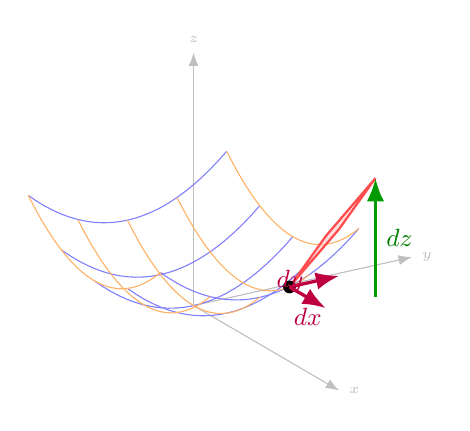
\begin{tikzpicture}[>=Latex,scale=1.4,x={(0.6cm,-0.35cm)},y={(0.9cm,0.2cm)},z={(0cm,0.85cm)}]
  \draw[->,gray!50] (0,0,0) -- (2.2,0,0) node[right,font=\tiny]{$x$};
  \draw[->,gray!50] (0,0,0) -- (0,2.2,0) node[right,font=\tiny]{$y$};
  \draw[->,gray!50] (0,0,0) -- (0,0,2.7) node[above,font=\tiny]{$z$};
  \foreach \u in {-1.0,-0.5,0,0.5,1.0}{\draw[blue!50,thin,domain=-1.0:1.0,samples=25] plot ({\u},{\x},{0.5*(\u*\u+\x*\x)});}
  \foreach \v in {-1.0,-0.5,0,0.5,1.0}{\draw[orange!60,thin,domain=-1.0:1.0,samples=25] plot ({\x},{\v},{0.5*(\x*\x+\v*\v)});}
  \pgfmathsetmacro{\xa}{0.7}\pgfmathsetmacro{\ya}{0.5}\pgfmathsetmacro{\za}{0.5*(\xa*\xa+\ya*\ya)}
  % Larger tangent plane patch
  \pgfmathsetmacro{\dxx}{0.55}\pgfmathsetmacro{\dyy}{0.5}\pgfmathsetmacro{\dzz}{2*\xa*\dxx+2*\ya*\dyy}
  \fill[red!25,opacity=0.5] (\xa,\ya,\za) -- ({\xa+\dxx},\ya,{\za+2*\xa*\dxx}) -- ({\xa+\dxx},{\ya+\dyy},{\za+\dzz}) -- (\xa,{\ya+\dyy},{\za+2*\ya*\dyy}) -- cycle;
  \draw[red!70,thick] (\xa,\ya,\za) -- ({\xa+\dxx},\ya,{\za+2*\xa*\dxx}) -- ({\xa+\dxx},{\ya+\dyy},{\za+\dzz}) -- (\xa,{\ya+\dyy},{\za+2*\ya*\dyy}) -- cycle;
  \filldraw[black] (\xa,\ya,\za) circle (1.5pt);
  \draw[->,purple,very thick] (\xa,\ya,\za) -- ({\xa+\dxx},\ya,\za) node[midway,below,font=\small,purple]{$dx$};
  \draw[->,purple,very thick] (\xa,\ya,\za) -- (\xa,{\ya+\dyy},\za) node[midway,left,font=\small,purple]{$dy$};
  \draw[->,green!60!black,very thick] ({\xa+\dxx},{\ya+\dyy},\za) -- ({\xa+\dxx},{\ya+\dyy},{\za+\dzz}) node[midway,right,font=\small,green!50!black]{$dz$};
\end{tikzpicture}
\end{center}

\textit{Tangent plane $=$ best linear approximation; error vanishes faster than $|\Delta\vec x|$.}

\begin{thm}
$f_x$, $f_y$ exist and are continuous near $(a,b)$ $\implies$ $f$ is differentiable at $(a,b)$.
\end{thm}

\textbf{Total differential.} $dz = \dfrac{\partial z}{\partial x}\,dx + \dfrac{\partial z}{\partial y}\,dy$. use to estimate errors, $\Delta z \approx dz$.

\textit{Picture.} $dz$ is the rise along the tangent plane, $\Delta z$ is the actual rise on the surface. their difference is second-order small.

\begin{center}
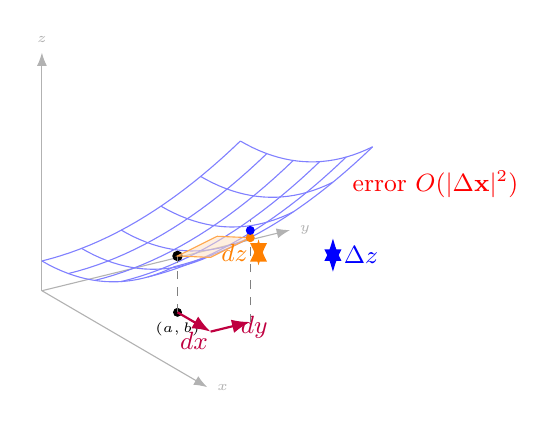
\begin{tikzpicture}[>=Latex,scale=1.4,x={(0.6cm,-0.35cm)},y={(0.9cm,0.22cm)},z={(0cm,0.9cm)}]
  \draw[->,gray!60] (0,0,0)--(2.5,0,0) node[right,font=\tiny]{$x$};
  \draw[->,gray!60] (0,0,0)--(0,2.5,0) node[right,font=\tiny]{$y$};
  \draw[->,gray!60] (0,0,0)--(0,0,2.4) node[above,font=\tiny]{$z$};
  % Surface z = 0.3 + 0.18(x^2+y^2)
  \foreach \u in {0,0.4,0.8,1.2,1.6,2.0}{
    \draw[blue!50,thin,domain=0:2.0,samples=22,variable=\v] plot (\u,\v,{0.3+0.18*(\u*\u+\v*\v)});
  }
  \foreach \v in {0,0.4,0.8,1.2,1.6,2.0}{
    \draw[blue!50,thin,domain=0:2.0,samples=22,variable=\u] plot (\u,\v,{0.3+0.18*(\u*\u+\v*\v)});
  }
  % Sample point (a,b) = (1, 0.7)
  \pgfmathsetmacro{\xa}{1.0}\pgfmathsetmacro{\yb}{0.7}
  \pgfmathsetmacro{\za}{0.3+0.18*(\xa*\xa+\yb*\yb)}
  \pgfmathsetmacro{\fxv}{2*0.18*\xa}\pgfmathsetmacro{\fyv}{2*0.18*\yb}
  \filldraw[black] (\xa,\yb,\za) circle (1.2pt);
  \filldraw[black] (\xa,\yb,0) circle (1pt) node[below,font=\tiny]{$(a,b)$};
  \draw[gray,dashed] (\xa,\yb,0)--(\xa,\yb,\za);
  % dx, dy increments
  \pgfmathsetmacro{\dxx}{0.5}\pgfmathsetmacro{\dyy}{0.4}
  \pgfmathsetmacro{\nx}{\xa+\dxx}\pgfmathsetmacro{\ny}{\yb+\dyy}
  \pgfmathsetmacro{\zT}{\za + \fxv*\dxx + \fyv*\dyy}
  \pgfmathsetmacro{\zS}{0.3+0.18*(\nx*\nx+\ny*\ny)}
  % Tangent plane patch
  \fill[orange!25,opacity=0.5] (\xa,\yb,\za)--(\nx,\yb,{\za+\fxv*\dxx})
       --(\nx,\ny,\zT)--(\xa,\ny,{\za+\fyv*\dyy})--cycle;
  \draw[orange!70] (\xa,\yb,\za)--(\nx,\yb,{\za+\fxv*\dxx})
       --(\nx,\ny,\zT)--(\xa,\ny,{\za+\fyv*\dyy})--cycle;
  % dx, dy arrows
  \draw[->,purple,thick] (\xa,\yb,0)--(\nx,\yb,0) node[midway,below,font=\small,purple]{$dx$};
  \draw[->,purple,thick] (\nx,\yb,0)--(\nx,\ny,0) node[midway,right,font=\small,purple]{$dy$};
  \draw[gray,dashed] (\nx,\ny,0)--(\nx,\ny,{\zS+0.1});
  % dz (tangent plane corner) and Delta z (surface)
  \filldraw[orange] (\nx,\ny,\zT) circle (1pt);
  \filldraw[blue] (\nx,\ny,\zS) circle (1pt);
  \draw[<->,orange,very thick] ({\nx+0.05},{\ny+0.05},\za)--({\nx+0.05},{\ny+0.05},\zT) node[midway,left,orange,font=\small\bfseries]{$dz$};
  \draw[<->,blue,very thick] ({\nx+0.5},{\ny+0.5},\za)--({\nx+0.5},{\ny+0.5},\zS) node[midway,right,blue,font=\small\bfseries]{$\Delta z$};
  \node[red,font=\small] at ({\nx+1.3},{\ny+1.0},{\zT+0.8}){error $O(|\Delta\vec x|^2)$};
\end{tikzpicture}
\end{center}

\medskip\textbf{Practice.}
\begin{enumerate}[noitemsep]
  \item Find the tangent plane to $x^2+2y^2+3z^2=21$ at the point $(2,2,1)$.
  \item Find the linear approximation of $f(x,y)=\sqrt{20-x^2-7y^2}$ at $(2,1)$ and use it to estimate $f(1.95,1.08)$.
\end{enumerate}

\subsection{14.5 The Chain Rule}

\textbf{Case 1} ($z=f(x,y)$, $x=g(t)$, $y=h(t)$):
\[
\frac{dz}{dt} = \frac{\partial z}{\partial x}\frac{dx}{dt}+\frac{\partial z}{\partial y}\frac{dy}{dt}
\]

\textbf{General version} ($z=f(x,y)$, $x=g(s,t)$, $y=h(s,t)$):
\[
\frac{\partial z}{\partial s} = \frac{\partial z}{\partial x}\frac{\partial x}{\partial s}+\frac{\partial z}{\partial y}\frac{\partial y}{\partial s}
\]

\textbf{Implicit differentiation} from $F(x,y,z)=0$:
\[
\frac{\partial z}{\partial x} = -\frac{F_x}{F_z}, \qquad \frac{\partial z}{\partial y} = -\frac{F_y}{F_z}
\]


\medskip\textbf{Practice.}
\begin{enumerate}[noitemsep]
  \item Given $w=f(x,y)$ with $x=s+t$ and $y=s-t$, show that $\dfrac{\partial w}{\partial s}+\dfrac{\partial w}{\partial t}=2\dfrac{\partial f}{\partial x}$.
  \item Let $z=x^2y$, $x=r\cos\theta$, $y=r\sin\theta$. Find $\dfrac{\partial z}{\partial\theta}$ using the chain rule.
  \item Find $\dfrac{\partial z}{\partial x}$ and $\dfrac{\partial z}{\partial y}$ for $x^2+y^2+z^2=3xyz$.
\end{enumerate}

\begin{center}
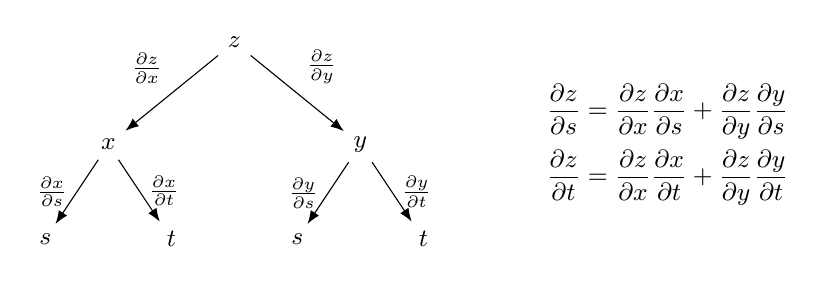
\begin{tikzpicture}[>=Latex,scale=1.0,every node/.style={font=\small}]
  % z=f(x,y), x=g(s,t), y=h(s,t)
  \node (z) at (0,2.5) {$z$};
  \node (x) at (-1.6,1.2) {$x$};
  \node (y) at (1.6,1.2) {$y$};
  \node (s1) at (-2.4,0) {$s$};
  \node (t1) at (-0.8,0) {$t$};
  \node (s2) at (0.8,0) {$s$};
  \node (t2) at (2.4,0) {$t$};
  \draw[->] (z) -- (x) node[midway,above left]{$\tfrac{\partial z}{\partial x}$};
  \draw[->] (z) -- (y) node[midway,above right]{$\tfrac{\partial z}{\partial y}$};
  \draw[->] (x) -- (s1) node[midway,left]{$\tfrac{\partial x}{\partial s}$};
  \draw[->] (x) -- (t1) node[midway,right]{$\tfrac{\partial x}{\partial t}$};
  \draw[->] (y) -- (s2) node[midway,left]{$\tfrac{\partial y}{\partial s}$};
  \draw[->] (y) -- (t2) node[midway,right]{$\tfrac{\partial y}{\partial t}$};
  \node[align=left,font=\small] at (5.5,1.2)
    {$\dfrac{\partial z}{\partial s}=\dfrac{\partial z}{\partial x}\dfrac{\partial x}{\partial s}+\dfrac{\partial z}{\partial y}\dfrac{\partial y}{\partial s}$\\[3pt]
     $\dfrac{\partial z}{\partial t}=\dfrac{\partial z}{\partial x}\dfrac{\partial x}{\partial t}+\dfrac{\partial z}{\partial y}\dfrac{\partial y}{\partial t}$};
\end{tikzpicture}
\end{center}

\subsection{14.6 Directional Derivatives and the Gradient Vector}

\medskip\textbf{calc 1 recap.} $f'(x)$ is the rate of change along the $x$-axis. here $D_{\vec u}f$ is the rate of change in the $\vec u$ direction.

\textbf{Directional derivative} in direction of unit vector $\vec{u}=\vv{a,b}$
\[
D_{\vec{u}}f(x,y) = \grad f(x,y)\cdot\vec{u} = f_x a + f_y b
\]

\begin{center}
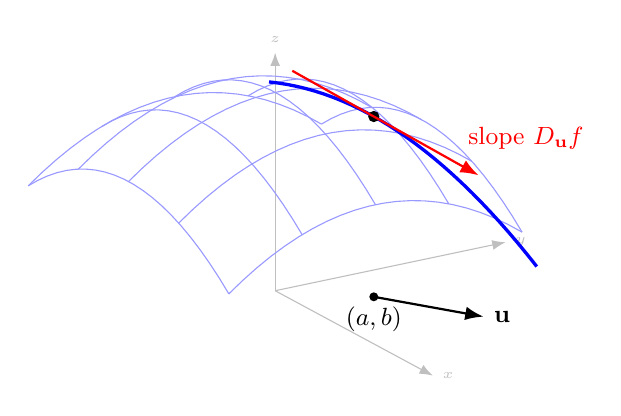
\begin{tikzpicture}[>=Latex,scale=1.4,x={(0.65cm,-0.35cm)},y={(0.95cm,0.2cm)},z={(0cm,0.9cm)}]
  \draw[->,gray!50] (0,0,0)--(2.2,0,0) node[right,font=\tiny]{$x$};
  \draw[->,gray!50] (0,0,0)--(0,2.2,0) node[right,font=\tiny]{$y$};
  \draw[->,gray!50] (0,0,0)--(0,0,2.4) node[above,font=\tiny]{$z$};
  % Surface z = 2 - 0.3(x^2+y^2)
  \foreach \u in {-1.4,-0.7,0,0.7,1.4}{
    \draw[blue!40,thin,domain=-1.4:1.4,samples=22,variable=\v] plot (\u,\v,{2-0.3*(\u*\u+\v*\v)});
  }
  \foreach \v in {-1.4,-0.7,0,0.7,1.4}{
    \draw[blue!40,thin,domain=-1.4:1.4,samples=22,variable=\u] plot (\u,\v,{2-0.3*(\u*\u+\v*\v)});
  }
  % Sample point and direction in xy-plane
  \pgfmathsetmacro{\sa}{0.5}\pgfmathsetmacro{\sb}{0.6}
  \draw[->,thick] (\sa,\sb,0) -- (\sa+0.8,\sb+0.5,0) node[right,font=\small]{$\vec u$};
  \filldraw (\sa,\sb,0) circle (1pt) node[below,font=\small]{$(a,b)$};
  % Vertical slice curve cut from surface along u direction
  \draw[blue,very thick,domain=-0.9:1.4,samples=30,variable=\s]
    plot ({\sa+0.85*\s},{\sb+0.53*\s},{2-0.3*((\sa+0.85*\s)*(\sa+0.85*\s)+(\sb+0.53*\s)*(\sb+0.53*\s))});
  % Tangent line at the sample point on the slice
  \pgfmathsetmacro{\zv}{2-0.3*(\sa*\sa+\sb*\sb)}
  \filldraw[black] (\sa,\sb,\zv) circle (1.3pt);
  % Slope = grad f . u_hat where u_hat = (0.85, 0.53, 0)/1 (already normalized roughly)
  \pgfmathsetmacro{\gx}{-0.6*\sa}\pgfmathsetmacro{\gy}{-0.6*\sb}
  \pgfmathsetmacro{\sl}{0.85*\gx+0.53*\gy}
  \draw[->,red,thick] ({\sa-0.7*0.85},{\sb-0.7*0.53},{\zv-0.7*\sl}) -- ({\sa+0.9*0.85},{\sb+0.9*0.53},{\zv+0.9*\sl});
  \node[red,font=\small] at (\sa+1.1,\sb+0.7,\zv+0.05){slope $D_{\vec u}f$};
\end{tikzpicture}
\end{center}

\textbf{Gradient.} $\grad f = \vv{f_x,f_y}$ in $\R^2$, $\vv{f_x,f_y,f_z}$ in $\R^3$.

\begin{thm}
$\max_{\vec{u}} D_{\vec{u}}f = |\grad f|$, hit when $\vec{u} = \grad f/|\grad f|$.
\end{thm}

$\grad f \perp$ level curves in $\R^2$, $\grad F \perp$ level surfaces in $\R^3$.

\textbf{Tangent plane to $F(x,y,z)=k$ at $(x_0,y_0,z_0)$}
\[
\grad F(x_0,y_0,z_0)\cdot\vv{x-x_0,y-y_0,z-z_0} = 0
\]

\textit{same as 14.4.} the graph $z=f(x,y)$ is the level set $F=z-f=0$, so $\grad F=\vv{-f_x,-f_y,1}$ and the formula collapses to $z-z_0=f_x(x-x_0)+f_y(y-y_0)$.

\begin{center}
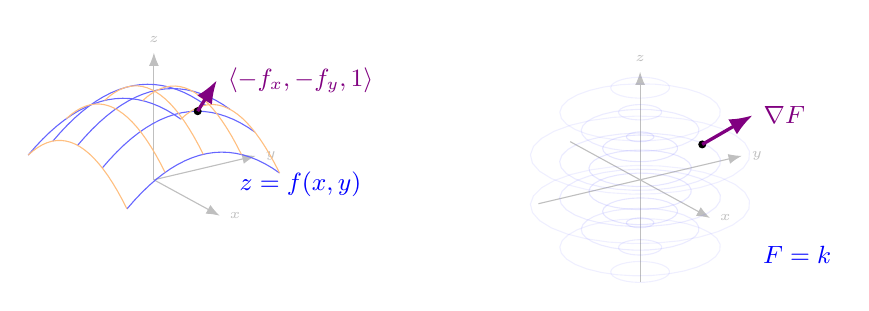
\begin{tikzpicture}[>=Latex,scale=0.95,x={(0.55cm,-0.3cm)},y={(0.85cm,0.2cm)},z={(0cm,0.85cm)}]
  \begin{scope}
    % z=f(x,y) as a proper surface mesh: bowl down (1.4 - 0.4(x^2+y^2))
    \draw[->,gray!50,thin] (0,0,0)--(1.6,0,0) node[right,font=\tiny]{$x$};
    \draw[->,gray!50,thin] (0,0,0)--(0,1.6,0) node[right,font=\tiny]{$y$};
    \draw[->,gray!50,thin] (0,0,0)--(0,0,2.0) node[above,font=\tiny]{$z$};
    \foreach \u in {-1.2,-0.6,0,0.6,1.2}
      \draw[blue!60,thin,domain=-1.2:1.2,samples=22,variable=\v] plot (\u,\v,{1.4-0.4*(\u*\u+\v*\v)});
    \foreach \v in {-1.2,-0.6,0,0.6,1.2}
      \draw[orange!50,thin,domain=-1.2:1.2,samples=22,variable=\u] plot (\u,\v,{1.4-0.4*(\u*\u+\v*\v)});
    % sample point at (0.6, 0.3)
    \pgfmathsetmacro{\sa}{0.6}\pgfmathsetmacro{\sb}{0.3}\pgfmathsetmacro{\sz}{1.4-0.4*(\sa*\sa+\sb*\sb)}
    \filldraw[black] (\sa,\sb,{\sz}) circle (1.3pt);
    \draw[->,violet,very thick] (\sa,\sb,{\sz})--({\sa+0.55*0.8*\sa},{\sb+0.55*0.8*\sb},{\sz+0.55*1.0}) node[right,violet,font=\small]{$\vv{-f_x,-f_y,1}$};
    \node[blue,font=\small] at (1.4,1.4,0.1){$z=f(x,y)$};
  \end{scope}
  \begin{scope}[xshift=6.5cm]
    % 3D level surfaces F=k: nested ellipsoids
    \draw[->,gray!50,thin] (-1.7,0,0)--(1.7,0,0) node[right,font=\tiny]{$x$};
    \draw[->,gray!50,thin] (0,-1.6,0)--(0,1.6,0) node[right,font=\tiny]{$y$};
    \draw[->,gray!50,thin] (0,0,-1.6)--(0,0,1.7) node[above,font=\tiny]{$z$};
    \foreach \k/\op in {0.7/0.16, 1.1/0.13, 1.5/0.10}{
      \foreach \phi in {15,45,...,165}
        \draw[blue!60,thin,opacity=\op,domain=0:360,samples=30,variable=\t]
          plot ({\k*sin(\phi)*cos(\t)},{\k*sin(\phi)*sin(\t)},{\k*cos(\phi)});
    }
    \pgfmathsetmacro{\ka}{1.1}
    \filldraw[black] ({\ka*0.6},{\ka*0.5},{\ka*0.6}) circle (1.3pt);
    \draw[->,violet,very thick] ({\ka*0.6},{\ka*0.5},{\ka*0.6})--({\ka*1.1},{\ka*0.9},{\ka*1.1}) node[right,violet,font=\small]{$\grad F$};
    \node[blue,font=\small] at (1.5,1.5,-1.0){$F=k$};
  \end{scope}
\end{tikzpicture}
\end{center}

\textit{gradient on contour map projects up to steepest ascent on the surface.} $\nabla f$ lives in $xy$ perp to a contour. the curve on $z=f$ directly above the $\nabla f$ line is the steepest path up.

\begin{center}
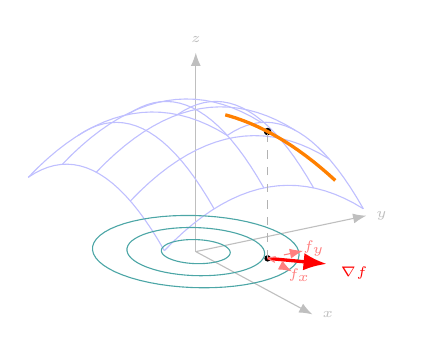
\begin{tikzpicture}[>=Latex,scale=0.95,x={(0.65cm,-0.35cm)},y={(0.95cm,0.2cm)},z={(0cm,0.95cm)}]
  \draw[->,gray!50] (0,0,0)--(2.4,0,0) node[right,font=\tiny]{$x$};
  \draw[->,gray!50] (0,0,0)--(0,2.4,0) node[right,font=\tiny]{$y$};
  \draw[->,gray!50] (0,0,0)--(0,0,2.8) node[above,font=\tiny]{$z$};
  % Surface z = 2 - 0.3(x^2 + y^2) gridded faintly
  \foreach \u in {-1.4,-0.7,0,0.7,1.4}{
    \draw[blue!25,thin,domain=-1.4:1.4,samples=22,variable=\v] plot (\u,\v,{2-0.3*(\u*\u+\v*\v)});
  }
  \foreach \v in {-1.4,-0.7,0,0.7,1.4}{
    \draw[blue!25,thin,domain=-1.4:1.4,samples=22,variable=\u] plot (\u,\v,{2-0.3*(\u*\u+\v*\v)});
  }
  % Level curves in xy plane
  \foreach \r in {0.4,0.8,1.2}{
    \draw[teal!70,domain=0:360,samples=60,variable=\t] plot ({\r*cos(\t)},{\r*sin(\t)},0);
  }
  % Sample point in xy-plane
  \pgfmathsetmacro{\sa}{0.6} \pgfmathsetmacro{\sb}{0.6}
  \pgfmathsetmacro{\zv}{2-0.3*(\sa*\sa+\sb*\sb)}
  \filldraw[black] (\sa,\sb,0) circle (1pt);
  % Gradient in xy-plane (radially outward)
  \pgfmathsetmacro{\nr}{sqrt(\sa*\sa+\sb*\sb)}
  \draw[->,red,very thick] (\sa,\sb,0) -- ({\sa+0.7*\sa/\nr},{\sb+0.7*\sb/\nr},0);
  \node[red,font=\tiny] at (1.5,1.2,0){$\nabla f$};
  % Show f_x and f_y components
  \draw[->,red!50,dashed] (\sa,\sb,0)--({\sa+0.5},\sb,0);
  \node[red!50,font=\tiny] at (1.25,\sb,0){$f_x$};
  \draw[->,red!50,dashed] (\sa,\sb,0)--(\sa,{\sb+0.5},0);
  \node[red!50,font=\tiny] at (\sa,1.25,0){$f_y$};
  % Point on surface above (a,b)
  \filldraw[black] (\sa,\sb,\zv) circle (1.2pt);
  \draw[dashed,gray!60] (\sa,\sb,0)--(\sa,\sb,\zv);
  % Steepest-ascent curve on surface: along radial direction at sample, project up
  \draw[orange,very thick,domain=-0.5:0.8,samples=30,variable=\s]
    plot ({\sa+\s*\sa/\nr},{\sb+\s*\sb/\nr},{2-0.3*((\sa+\s*\sa/\nr)*(\sa+\s*\sa/\nr)+(\sb+\s*\sb/\nr)*(\sb+\s*\sb/\nr))});
  \node[orange,font=\tiny] at ({\sa-0.6*\sa/\nr},{\sb-0.6*\sb/\nr},{2-0.3*((\sa-0.6*\sa/\nr)*(\sa-0.6*\sa/\nr)+(\sb-0.6*\sb/\nr)*(\sb-0.6*\sb/\nr))+0.2}){};
\end{tikzpicture}
\end{center}

\textit{3D case: level surfaces and gradient.} For a function $F(x,y,z)$ of three variables, level surfaces $F=k$ are 2D surfaces in 3D space. The gradient $\nabla F$ is always perpendicular to the level surface:

\begin{center}
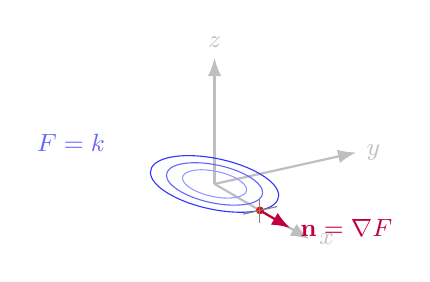
\begin{tikzpicture}[>=Latex,scale=0.8,x={(0.6cm,-0.35cm)},y={(0.9cm,0.2cm)},z={(0cm,0.8cm)}]
  % Labeled axes
  \draw[->,gray!50,thick] (0,0,0) -- (2.5,0,0) node[right,font=\small]{$x$};
  \draw[->,gray!50,thick] (0,0,0) -- (0,2.5,0) node[right,font=\small]{$y$};
  \draw[->,gray!50,thick] (0,0,0) -- (0,0,2.5) node[above,font=\small]{$z$};

  % Nested ellipsoids (level surfaces)
  % Innermost: smaller ellipsoid
  \draw[blue!40] (0,0,0) ellipse (0.6 and 0.4);

  % Middle: medium ellipsoid
  \draw[blue!60] (0,0,0) ellipse (0.9 and 0.6);

  % Outermost: larger ellipsoid
  \draw[blue!80] (0,0,0) ellipse (1.2 and 0.8);

  % Point on outermost level surface
  \filldraw[red] (1.2,0,0) circle (1.5pt);

  % Normal vector perpendicular to level surface (pointing outward along x-direction)
  \draw[->,thick,purple] (1.2,0,0) -- (2.0,0,0) node[right,font=\small]{$\vec n=\nabla F$};

  % Show tangent plane as a small orthogonal grid at the point
  \draw[gray,thin] (1.2,-0.3,0) -- (1.2,0.3,0);
  \draw[gray,thin] (1.2,0,-0.25) -- (1.2,0,0.25);

  % Labels
  \node[blue!60,font=\small] at (-1.4,-1.6,0.6){$F=k$};
\end{tikzpicture}
\end{center}

\medskip\textbf{Practice.}
\begin{enumerate}[noitemsep]
  \item Find the directional derivative of $f(x,y)=x^2y^3$ at $P(1,2)$ in the direction of $\vec{v}=\ihat+\jhat$.
  \item Find the maximum rate of change of $f(x,y,z)=x+y/z$ at $(1,1,1)$ and the direction in which it occurs.
  \item Sketch the level curves of $f(x,y)=x^2+y^2$. At the point $(1,1)$, draw the gradient vector $\nabla f$ and explain why it is perpendicular to the level curve through that point.
\end{enumerate}

\subsection{14.7 Maximum and Minimum Values}

\medskip\textbf{calc 1 recap.} for $y=f(x)$ extrema sit at $f'(x)=0$, classified by sign of $f''$. in 2 variables we use $f_x,f_y$ instead and the hessian (2nd partials) classifies.

\textbf{Critical point.} $(a,b)$ with $f_x=f_y=0$, or a partial DNE.

\begin{thm}
Local extremum at $(a,b)$ $\implies$ $(a,b)$ is a critical point.
\end{thm}

\begin{thm}[Second Derivatives Test]
Let $D = f_{xx}f_{yy}-(f_{xy})^2$ at critical point $(a,b)$:
\begin{itemize}[noitemsep]
\item $D>0$, $f_{xx}>0$: local minimum
\item $D>0$, $f_{xx}<0$: local maximum
\item $D<0$: saddle point
\item $D=0$: test inconclusive
\end{itemize}
\end{thm}

\textbf{Extreme Value Theorem.} continuous $f$ on closed bounded $D$ attains its max and min.

\textbf{strategy for absolute extrema.} interior critical points, then evaluate on the boundary then compare.

\medskip\textbf{3D pictures.} three cases: min (paraboloid up), max (paraboloid down), saddle (hyperbolic paraboloid).

\begin{center}
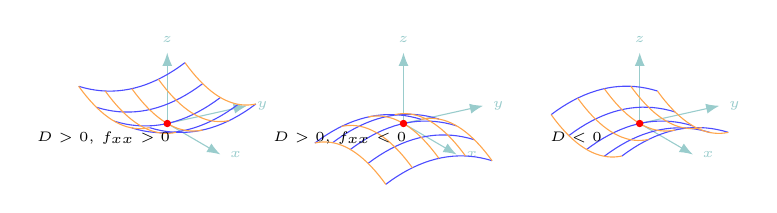
\begin{tikzpicture}[>=Latex,scale=0.75,x={(0.6cm,-0.35cm)},y={(0.9cm,0.2cm)},z={(0cm,0.8cm)}]
  % Local minimum: paraboloid opening up
  \begin{scope}
    \draw[->,teal!40,thin] (0,0,0) -- (1.5,0,0) node[right,font=\tiny]{$x$};
    \draw[->,teal!40,thin] (0,0,0) -- (0,1.5,0) node[right,font=\tiny]{$y$};
    \draw[->,teal!40,thin] (0,0,0) -- (0,0,1.5) node[above,font=\tiny]{$z$};
    \foreach \u in {-1,-0.5,0,0.5,1}{\draw[blue!70,domain=-1:1,samples=20] plot ({\u},{\x},{0.3*(\u*\u+\x*\x)});}
    \foreach \v in {-1,-0.5,0,0.5,1}{\draw[orange!70,domain=-1:1,samples=20] plot ({\x},{\v},{0.3*(\x*\x+\v*\v)});}
    \filldraw[red] (0,0,0) circle (1.5pt);
    \node[font=\tiny] at (0,-1.2){$D>0,\,f_{xx}>0$};
  \end{scope}
  % Local maximum: paraboloid opening down
  \begin{scope}[xshift=4cm]
    \draw[->,teal!40,thin] (0,0,0) -- (1.5,0,0) node[right,font=\tiny]{$x$};
    \draw[->,teal!40,thin] (0,0,0) -- (0,1.5,0) node[right,font=\tiny]{$y$};
    \draw[->,teal!40,thin] (0,0,0) -- (0,0,1.5) node[above,font=\tiny]{$z$};
    \foreach \u in {-1,-0.5,0,0.5,1}{\draw[blue!70,domain=-1:1,samples=20] plot ({\u},{\x},{-0.3*(\u*\u+\x*\x)});}
    \foreach \v in {-1,-0.5,0,0.5,1}{\draw[orange!70,domain=-1:1,samples=20] plot ({\x},{\v},{-0.3*(\x*\x+\v*\v)});}
    \filldraw[red] (0,0,0) circle (1.5pt);
    \node[font=\tiny] at (0,-1.2){$D>0,\,f_{xx}<0$};
  \end{scope}
  % Saddle point: hyperbolic paraboloid
  \begin{scope}[xshift=8cm]
    \draw[->,teal!40,thin] (0,0,0) -- (1.5,0,0) node[right,font=\tiny]{$x$};
    \draw[->,teal!40,thin] (0,0,0) -- (0,1.5,0) node[right,font=\tiny]{$y$};
    \draw[->,teal!40,thin] (0,0,0) -- (0,0,1.5) node[above,font=\tiny]{$z$};
    \foreach \u in {-1,-0.5,0,0.5,1}{\draw[blue!70,domain=-1:1,samples=20] plot ({\u},{\x},{0.3*(\u*\u-\x*\x)});}
    \foreach \v in {-1,-0.5,0,0.5,1}{\draw[orange!70,domain=-1:1,samples=20] plot ({\x},{\v},{0.3*(\x*\x-\v*\v)});}
    \filldraw[red] (0,0,0) circle (1.5pt);
    \node[font=\tiny] at (0,-1.2){$D<0$};
  \end{scope}
\end{tikzpicture}
\end{center}

\medskip\textbf{Hessian and eigenvalues.} the hessian $H = \begin{pmatrix} f_{xx} & f_{xy} \\ f_{xy} & f_{yy} \end{pmatrix}$ captures the second-order behavior at a critical point. its eigenvalues $\lambda_1,\lambda_2$ are the curvatures along the principal directions.
\begin{itemize}[noitemsep]
\item both $\lambda_i > 0$, local min, paraboloid opens up everywhere.
\item both $\lambda_i < 0$, local max, opens down everywhere.
\item $\lambda_1>0$ and $\lambda_2<0$ saddle, up one way down the other.
\end{itemize}
$D=\det H=\lambda_1\lambda_2$ and the sign of $f_{xx}$ pin down the case.

\textit{eigenvectors.} the eigenvectors of $H$ are the principal directions of curvature. when $H$ is diagonal, those are $\ihat$ and $\jhat$. when $f_{xy}\ne 0$, the principal directions tilt away from the coordinate axes. the surface looks the same as the diagonal case, just rotated.

\begin{center}
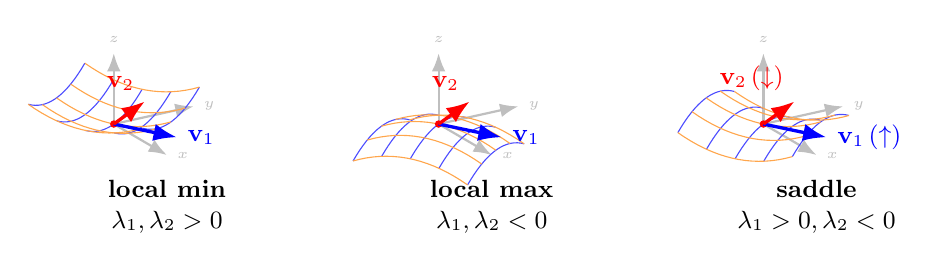
\begin{tikzpicture}[>=Latex,scale=0.75,x={(0.6cm,-0.35cm)},y={(0.9cm,0.2cm)},z={(0cm,0.8cm)}]
  % Min in rotated frame
  \begin{scope}
    \draw[->,gray!50,thick] (0,0,0)--(1.5,0,0) node[right,font=\tiny]{$x$};
    \draw[->,gray!50,thick] (0,0,0)--(0,1.5,0) node[right,font=\tiny]{$y$};
    \draw[->,gray!50,thick] (0,0,0)--(0,0,1.5) node[above,font=\tiny]{$z$};
    % rotated paraboloid grid: u,v are eigenvector dirs at 30 deg
    \foreach \uu in {-1,-0.5,0,0.5,1}{
      \draw[blue!70,thin,domain=-1:1,samples=18,variable=\vv]
        plot ({\uu*cos(30)-\vv*sin(30)},{\uu*sin(30)+\vv*cos(30)},{0.3*(\uu*\uu+\vv*\vv)});
    }
    \foreach \vv in {-1,-0.5,0,0.5,1}{
      \draw[orange!70,thin,domain=-1:1,samples=18,variable=\uu]
        plot ({\uu*cos(30)-\vv*sin(30)},{\uu*sin(30)+\vv*cos(30)},{0.3*(\uu*\uu+\vv*\vv)});
    }
    \filldraw[red] (0,0,0) circle (1.5pt);
    % Eigenvector arrows at origin in xy-plane (rotated 30 deg from axes)
    \draw[->,very thick,blue] (0,0,0)--({1.1*cos(30)},{1.1*sin(30)},0) node[right,font=\small,blue]{$\vec v_1$};
    \draw[->,very thick,red] (0,0,0)--({-1.1*sin(30)},{1.1*cos(30)},0) node[above left,font=\small,red]{$\vec v_2$};
    \node[font=\small,align=center] at (0,1.0,-2.0){\textbf{local min}\\$\lambda_1,\lambda_2>0$};
  \end{scope}
  \begin{scope}[xshift=5.5cm]
    \draw[->,gray!50,thick] (0,0,0)--(1.5,0,0) node[right,font=\tiny]{$x$};
    \draw[->,gray!50,thick] (0,0,0)--(0,1.5,0) node[right,font=\tiny]{$y$};
    \draw[->,gray!50,thick] (0,0,0)--(0,0,1.5) node[above,font=\tiny]{$z$};
    \foreach \uu in {-1,-0.5,0,0.5,1}{
      \draw[blue!70,thin,domain=-1:1,samples=18,variable=\vv]
        plot ({\uu*cos(30)-\vv*sin(30)},{\uu*sin(30)+\vv*cos(30)},{-0.3*(\uu*\uu+\vv*\vv)});
    }
    \foreach \vv in {-1,-0.5,0,0.5,1}{
      \draw[orange!70,thin,domain=-1:1,samples=18,variable=\uu]
        plot ({\uu*cos(30)-\vv*sin(30)},{\uu*sin(30)+\vv*cos(30)},{-0.3*(\uu*\uu+\vv*\vv)});
    }
    \filldraw[red] (0,0,0) circle (1.5pt);
    \draw[->,very thick,blue] (0,0,0)--({1.1*cos(30)},{1.1*sin(30)},0) node[right,font=\small,blue]{$\vec v_1$};
    \draw[->,very thick,red] (0,0,0)--({-1.1*sin(30)},{1.1*cos(30)},0) node[above left,font=\small,red]{$\vec v_2$};
    \node[font=\small,align=center] at (0,1.0,-2.0){\textbf{local max}\\$\lambda_1,\lambda_2<0$};
  \end{scope}
  \begin{scope}[xshift=11cm]
    \draw[->,gray!50,thick] (0,0,0)--(1.5,0,0) node[right,font=\tiny]{$x$};
    \draw[->,gray!50,thick] (0,0,0)--(0,1.5,0) node[right,font=\tiny]{$y$};
    \draw[->,gray!50,thick] (0,0,0)--(0,0,1.5) node[above,font=\tiny]{$z$};
    \foreach \uu in {-1,-0.5,0,0.5,1}{
      \draw[blue!70,thin,domain=-1:1,samples=18,variable=\vv]
        plot ({\uu*cos(30)-\vv*sin(30)},{\uu*sin(30)+\vv*cos(30)},{0.3*(\uu*\uu-\vv*\vv)});
    }
    \foreach \vv in {-1,-0.5,0,0.5,1}{
      \draw[orange!70,thin,domain=-1:1,samples=18,variable=\uu]
        plot ({\uu*cos(30)-\vv*sin(30)},{\uu*sin(30)+\vv*cos(30)},{0.3*(\uu*\uu-\vv*\vv)});
    }
    \filldraw[red] (0,0,0) circle (1.5pt);
    \draw[->,very thick,blue] (0,0,0)--({1.1*cos(30)},{1.1*sin(30)},0) node[right,font=\small,blue]{$\vec v_1\,(\uparrow)$};
    \draw[->,very thick,red] (0,0,0)--({-1.1*sin(30)},{1.1*cos(30)},0) node[above left,font=\small,red]{$\vec v_2\,(\downarrow)$};
    \node[font=\small,align=center] at (0,1.0,-2.0){\textbf{saddle}\\$\lambda_1>0,\lambda_2<0$};
  \end{scope}
\end{tikzpicture}
\end{center}

\medskip\textbf{Practice.}
\begin{enumerate}[noitemsep]
  \item Find and classify the critical points of $f(x,y)=x^4+y^4-4xy+1$.
  \item Find the absolute maximum and minimum of $f(x,y)=xy$ on the closed disk $x^2+y^2\le 1$.
  \item Find three positive numbers whose sum is $100$ and whose product is a maximum.
\end{enumerate}

\subsection{14.8 Lagrange Multipliers}

\textbf{Setup.} optimize $f(x,y)$ subject to $g(x,y)=k$. at an extremum the level curve of $f$ is tangent to the constraint, so $\nabla f\parallel\nabla g$.
\[
\nabla f=\lambda\nabla g,\qquad g=k.
\]
Solve the system; compare $f$ at all candidates.

\begin{center}
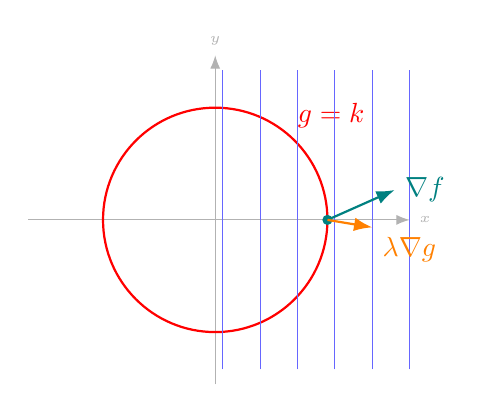
\begin{tikzpicture}[>=Latex,scale=0.95]
  \draw[->,gray!60] (-2.5,0)--(2.6,0) node[right,font=\tiny]{$x$};
  \draw[->,gray!60] (0,-2.2)--(0,2.2) node[above,font=\tiny]{$y$};
  % constraint curve
  \draw[thick,red] (0,0) circle (1.5);
  \node[red] at (1.55,1.4){$g=k$};
  % level curves of f
  \foreach \k in {-1.0,-0.5,0,0.5,1.0,1.5} {
    \draw[blue!60] (\k+1.1,-2) -- (\k+1.1,2);
  }
  % tangency point
  \filldraw[teal] (1.5,0) circle (1.7pt);
  \draw[->,thick,teal] (1.5,0) -- (2.4,0.4) node[right]{$\nabla f$};
  \draw[->,thick,orange] (1.5,0) -- (2.1,-0.1) node[below right,orange]{$\lambda\nabla g$};
\end{tikzpicture}
\end{center}

\textit{example.} Max/min of $f=xy$ on $x^2+y^2=8$: $\vv{y,x}=\lambda\vv{2x,2y}\Rightarrow x^2=y^2$, then $2x^2=8\Rightarrow x=\pm 2$. Max $f=4$ at same-sign points, min $-4$ at opposite-sign.

\textbf{Two constraints in $\R^3$.} $\nabla f=\lambda\nabla g+\mu\nabla h$ (gradient lies in plane spanned by the two normals).

\medskip
\textit{Second-derivative test, why it works.} At a critical point ($f_x=f_y=0$), moving in direction $\vec u$ has second derivative $\vec u^\top H\vec u$ where $H$ is the Hessian. The arrows below show in which directions $f$ increases (blue) vs decreases (red); $D=\det H$ and $f_{xx}$ tell you which case:

\begin{center}
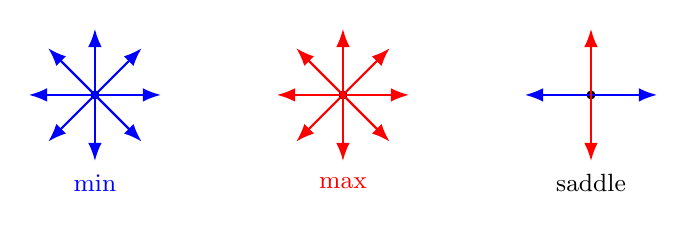
\begin{tikzpicture}[>=Latex,scale=0.7]
  \begin{scope}
    \filldraw (0,0) circle (2pt);
    \foreach \a in {0,45,...,315} \draw[->,blue,thick] (0,0) -- (\a:1.2);
    \node[blue] at (0,-1.6){\small min};
  \end{scope}
  \begin{scope}[xshift=4.5cm]
    \filldraw (0,0) circle (2pt);
    \foreach \a in {0,45,...,315} \draw[->,red,thick] (0,0) -- (\a:1.2);
    \node[red] at (0,-1.6){\small max};
  \end{scope}
  \begin{scope}[xshift=9cm]
    \filldraw (0,0) circle (2pt);
    \foreach \a in {0,180} \draw[->,blue,thick] (0,0) -- (\a:1.2);
    \foreach \a in {90,270} \draw[->,red,thick] (0,0) -- (\a:1.2);
    \node at (0,-1.6){\small saddle};
  \end{scope}
\end{tikzpicture}
\end{center}

\medskip\textbf{Practice.}
\begin{enumerate}[noitemsep]
  \item Use Lagrange multipliers to find the maximum and minimum values of $f(x,y)=x^2+y^2$ subject to $xy=1$.
  \item Find the maximum and minimum values of $f(x,y)=3x+y$ on the circle $x^2+y^2=10$.
  \item Find the point on the plane $x-y+z=4$ closest to $(1,2,3)$.
\end{enumerate}

\subsection{14.9 Taylor Approximation for Surfaces}

\textbf{Taylor series for functions of two variables.} near a point $(x_0, y_0)$, the function $f(x,y)$ can be approximated by a polynomial:
\[
f(x_0+h, y_0+k) \approx f(x_0,y_0) + f_x(x_0,y_0) \cdot h + f_y(x_0,y_0) \cdot k + \tfrac{1}{2}\big(f_{xx}(x_0,y_0) h^2 + 2f_{xy}(x_0,y_0) hk + f_{yy}(x_0,y_0) k^2\big) + \cdots
\]

The first-order terms define the tangent plane; the second-order terms capture how the surface curves away from it (determined by the Hessian).

\textit{example.} Take $f(x,y)=\sin x+\cos y$ at $(0,0)$ with $f(0,0)=1$, $f_x=\cos x$, $f_y=-\sin y$, $f_{xx}=-\sin x$, $f_{yy}=-\cos y$, $f_{xy}=0$.
At $(0,0)$: $L(x,y)=1+x$ (tangent plane, tilts in $x$, flat in $y$), $Q(x,y)=1+x-\tfrac{y^2}{2}$ (osculating paraboloid, adds downward curvature in $y$).

\begin{center}
\begin{tikzpicture}[>=Latex,scale=1.6,x={(0.6cm,-0.3cm)},y={(0.92cm,0.22cm)},z={(0cm,0.9cm)}]
  \draw[->,gray!50] (-1.3,0,0)--(1.4,0,0) node[right,font=\tiny]{$x$};
  \draw[->,gray!50] (0,-1.2,0)--(0,1.4,0) node[right,font=\tiny]{$y$};
  \draw[->,gray!50] (0,0,-0.3)--(0,0,2.4) node[above,font=\tiny]{$z$};
  % Tangent plane L = 1 + x (flat in y) orange patch
  \fill[orange!25,opacity=0.55] (-0.9,-1.0,0.1)--(0.9,-1.0,1.9)--(0.9,1.0,1.9)--(-0.9,1.0,0.1)--cycle;
  \draw[orange!80] (-0.9,-1.0,0.1)--(0.9,-1.0,1.9)--(0.9,1.0,1.9)--(-0.9,1.0,0.1)--cycle;
  % Quadratic Q = 1 + x - y^2/2 -- denser green mesh so it reads as a surface
  \foreach \v in {-1.0,-0.75,-0.5,-0.25,0,0.25,0.5,0.75,1.0}
    \draw[green!55!black,line width=1.0pt,domain=-0.9:0.9,samples=26,variable=\u] plot (\u,\v,{1+\u-0.5*\v*\v});
  \foreach \u in {-0.9,-0.6,-0.3,0,0.3,0.6,0.9}
    \draw[green!55!black,line width=0.8pt,domain=-1.0:1.0,samples=26,variable=\v] plot (\u,\v,{1+\u-0.5*\v*\v});
  % Actual z = sin x + cos y — blue mesh, slightly opaque
  \foreach \v in {-1.0,-0.5,0,0.5,1.0}
    \draw[blue,very thick,domain=-1.0:1.0,samples=30,variable=\u] plot (\u,\v,{sin(\u r)+cos(\v r)});
  % Base point
  \filldraw[red] (0,0,1) circle (1.5pt);
  % Right-side labels
  \node[blue,font=\small] at (1.3,1.1,1.4){actual $f$};
  \node[orange,font=\small] at (1.3,-0.8,2.0){tangent plane $L$};
  \node[green!60!black,font=\small] at (-1.2,-1.0,0.0){osc.\ paraboloid $Q$};
\end{tikzpicture}
\end{center}

\textit{linear gives a flat plane. quadratic adds curvature. the actual surface is in between (or beyond) in the $y$ direction.}

\textit{Meaning.} The tangent plane is the first-order approximation; the osculating paraboloid (determined by the Hessian) is the second-order approximation. This is why the second-derivative test works: the Hessian eigenvalues tell us whether the surface curves away from the tangent plane in all directions (minimum/maximum) or in mixed directions (saddle point).

\medskip\textbf{Practice.}
\begin{enumerate}[noitemsep]
  \item Write the second-order Taylor approximation of $f(x,y)=e^{xy}$ near $(0,0)$.
  \item For $f(x,y)=\sin(x+y)$, find the tangent plane at $(0,0)$ and the second-order Taylor polynomial.
  \item Compute the first three terms of the Taylor series for $f(x,y)=\sqrt{1+x+y}$ near $(0,0)$.
\end{enumerate}

\newpage
%                       --
\section{Chapter 15: Multiple Integrals}
%                       --

\subsection{15.1 Double Integrals over Rectangles and Area/Volume}

\textbf{Part A. Area in 2D.} The area of $D$ bounded below by $y=g(x)$ and above by $y=f(x)$ on $[a,b]$ is
\[
A = \int_a^b (f(x)-g(x))\,dx = \iint_D 1\,dA.
\]

\begin{center}
\begin{tikzpicture}[>=Latex,scale=0.95]
  \draw[->,gray!60] (-0.3,0)--(3.5,0) node[right,font=\tiny]{$x$};
  \draw[->,gray!60] (0,-0.3)--(0,2.4) node[above,font=\tiny]{$y$};
  \fill[blue!20] plot[domain=0.3:3,samples=40] (\x,{1.2+0.5*\x}) -- (3,0.4) -- (0.3,0.4) -- cycle;
  \draw[thick,blue,domain=0.3:3,samples=40] plot (\x,{1.2+0.5*\x});
  \node[blue,font=\small] at (3.4,2.7){$y=f(x)$};
  \draw[thick,orange,domain=0.3:3,samples=40] plot (\x,{0.4});
  \node[orange,font=\small] at (3.4,0.45){$y=g(x)$};
  \foreach \xx in {0.8,1.5,2.2} {
    \pgfmathsetmacro{\topval}{1.2+0.5*\xx}
    \draw[red,thin] (\xx,0.4)--(\xx,\topval);
  }
\end{tikzpicture}
\end{center}

\textbf{Part B. Volume in 3D.} Take the \emph{same} region $D$ in the $xy$ plane and put a surface $z=h(x,y)$ above it. The volume between $D$ and the surface is
\[
V = \iint_D h(x,y)\,dA
\]
setting $h=f(x)-g(x)$ recovers part A as a prism of height equal to the gap.

\begin{center}
\begin{tikzpicture}[>=Latex,
  x={(0.85cm,0cm)}, y={(0.30cm,0.22cm)}, z={(0cm,0.85cm)}, scale=0.85]
  \draw[->,gray!50] (0,0,0)--(4,0,0) node[right,font=\tiny]{$x$};
  \draw[->,gray!50] (0,0,0)--(0,3.5,0) node[right,font=\tiny]{$y$};
  \draw[->,gray!50] (0,0,0)--(0,0,3) node[above,font=\tiny]{$z$};
  % Same Part A region in the xy-plane: x in [0.3,3], y from g(x)=0.4 to f(x)=1.2+0.5x
  \fill[blue!18]
    plot[domain=0.3:3,samples=40,variable=\u] (\u,{0.4},0)
    -- plot[domain=3:0.3,samples=40,variable=\u] (\u,{1.2+0.5*\u},0) -- cycle;
  \draw[orange,thick,domain=0.3:3,samples=40,variable=\u] plot (\u,{0.4},0);
  \draw[blue,thick,domain=0.3:3,samples=40,variable=\u] plot (\u,{1.2+0.5*\u},0);
  \node[font=\tiny] at (1.7,0.3,0){$D$};
  % Surface z = h(x,y) above the region as a curved bowl-mesh
  \foreach \u in {0.5,0.9,1.3,1.7,2.1,2.5,2.9} {
    \pgfmathsetmacro{\vmax}{1.2+0.5*\u}
    \draw[blue!60,thin,domain=0.4:\vmax,samples=20,variable=\v]
      plot (\u,\v,{0.6+0.2*\u+0.25*sin(deg(\v))+0.18*\u*\v*0.1});
  }
  \foreach \vstar in {0.6,1.0,1.4,1.8,2.2,2.6} {
    \draw[orange!70,thin,domain=0.3:3,samples=20,variable=\u]
      plot (\u,\vstar,{0.6+0.2*\u+0.25*sin(deg(\vstar))+0.18*\u*\vstar*0.1});
  }
  \node[blue!70,font=\small] at (3.4,2.5,2.0){$z=h(x,y)$};
  % side walls (thin vertical strips at corners to anchor it)
  \draw[gray!40,thin] (0.3,0.4,0)--(0.3,0.4,{0.6+0.2*0.3+0.25*sin(deg(0.4))});
  \draw[gray!40,thin] (3,0.4,0)--(3,0.4,{0.6+0.2*3+0.25*sin(deg(0.4))+0.054});
\end{tikzpicture}
\end{center}

\textbf{Riemann sum.} Chop the floor into tiny tiles. Put a column of height $f$ above each. Add up.

\begin{center}
\begin{tikzpicture}[>=Latex,
  x={(0.85cm,0cm)}, y={(0.30cm,0.22cm)}, z={(0cm,0.85cm)}, scale=0.9]
  \draw[->,gray] (0,0,0)--(4,0,0) node[right]{$x$};
  \draw[->,gray] (0,0,0)--(0,3.5,0) node[right]{$y$};
  \draw[->,gray] (0,0,0)--(0,0,3) node[above]{$z$};
  \fill[blue!15] (0,0,0)--(3,0,0)--(3,2.5,0)--(0,2.5,0)--cycle;
  \draw[blue!60,thick] (0,0,0)--(3,0,0)--(3,2.5,0)--(0,2.5,0)--cycle;
  \def\bx{1.3}\def\by{1.0}\def\h{2.2}
  \fill[orange!20] (\bx,\by,0)--(\bx+0.7,\by,0)--(\bx+0.7,\by,\h)--(\bx,\by,\h)--cycle;
  \fill[orange!15] (\bx+0.7,\by,0)--(\bx+0.7,\by+0.7,0)--(\bx+0.7,\by+0.7,\h)--(\bx+0.7,\by,\h)--cycle;
  \fill[orange!35] (\bx,\by,\h)--(\bx+0.7,\by,\h)--(\bx+0.7,\by+0.7,\h)--(\bx,\by+0.7,\h)--cycle;
  \draw[orange!80] (\bx,\by,\h)--(\bx+0.7,\by,\h)--(\bx+0.7,\by+0.7,\h)--(\bx,\by+0.7,\h)--cycle;
  \draw[orange!70] (\bx,\by,0)--(\bx,\by,\h);
  \draw[orange!70] (\bx+0.7,\by,0)--(\bx+0.7,\by,\h);
  \draw[orange!70] (\bx+0.7,\by+0.7,0)--(\bx+0.7,\by+0.7,\h);
  \draw[red,<->] (\bx+0.85,\by,0)--(\bx+0.85,\by,\h) node[midway,right,red]{\small$f(x^*,y^*)$};
  \filldraw[red] (\bx+0.35,\by+0.35,0) circle (1.2pt);
  \node[red,font=\tiny] at (\bx+0.35,\by+0.35,-0.3){$(x^*,y^*)$};
  \draw[thick,blue,domain=0:3,samples=40] plot (\x,0,{1.8+0.3*sin(\x r)+0.15*\x});
  \node[blue] at (3.2,0,2.5){$z{=}f$};
\end{tikzpicture}
\end{center}

Refining the tiles gives
\[
\iint_R f\,dA = \lim_{m,n\to\infty}\sum_{i,j}f(x_{ij}^*,y_{ij}^*)\Delta A.
\]

\begin{center}
\begin{tikzpicture}[>=Latex,
  x={(0.85cm,0cm)}, y={(0.30cm,0.22cm)}, z={(0cm,0.85cm)}, scale=0.9]
  \draw[->,gray] (0,0,0)--(4,0,0) node[right]{$x$};
  \draw[->,gray] (0,0,0)--(0,3.5,0) node[right]{$y$};
  \draw[->,gray] (0,0,0)--(0,0,2.8) node[above]{$z$};
  \foreach \bx/\by/\h in {
    0/2/1.3, 1/2/1.7, 2/2/1.4,
    0/1/1.7, 1/1/2.2, 2/1/1.8,
    0/0/1.4, 1/0/1.9, 2/0/1.6}{
    \fill[orange!25] (\bx,\by,0)--(\bx+1,\by,0)--(\bx+1,\by,\h)--(\bx,\by,\h)--cycle;
    \fill[orange!15] (\bx+1,\by,0)--(\bx+1,\by+1,0)--(\bx+1,\by+1,\h)--(\bx+1,\by,\h)--cycle;
    \fill[orange!35] (\bx,\by,\h)--(\bx+1,\by,\h)--(\bx+1,\by+1,\h)--(\bx,\by+1,\h)--cycle;
    \draw[orange!80,thin] (\bx,\by,\h)--(\bx+1,\by,\h)--(\bx+1,\by+1,\h)--(\bx,\by+1,\h)--cycle;
    \draw[orange!70,thin] (\bx,\by,0)--(\bx,\by,\h);
    \draw[orange!70,thin] (\bx+1,\by,0)--(\bx+1,\by,\h);
    \draw[orange!70,thin] (\bx+1,\by+1,0)--(\bx+1,\by+1,\h);
  }
  \draw[thick,blue,domain=0:3,samples=40] plot (\x,0,{1.4+0.3*sin(\x r)+0.15*\x});
  \node[blue] at (3.2,0,2.2){$z{=}f$};
\end{tikzpicture}
\end{center}

\begin{thm}[Fubini]
If $f$ is continuous on $R=[a,b]\times[c,d]$:
\[
\iint_R f\,dA = \int_a^b\int_c^d f(x,y)\,dy\,dx = \int_c^d\int_a^b f(x,y)\,dx\,dy
\]
\end{thm}

\textbf{Average value.} $\bar{f} = \dfrac{1}{A(R)}\iint_R f\,dA$

\medskip\textbf{Practice.}
\begin{enumerate}[noitemsep]
  \item Evaluate $\iint_{R}(x^2y+4)\,dA$ where $R=[0,3]\times[1,2]$.
  \item Calculate $\iint_{D}(x+y)\,dA$ where $D$ is the triangular region with vertices $(0,0),(1,0),(1,1)$.
\end{enumerate}

\subsection{15.2 Double Integrals over General Regions}

\begin{center}
\begin{tikzpicture}[>=Latex,scale=0.95]
  \begin{scope}
    \fill[blue!15] plot[domain=0:3,samples=40] (\x,{1.6-0.2*\x*\x+0.1*\x}) -- plot[domain=3:0,samples=40] (\x,{0.3+0.15*\x});
    \draw[thick,blue,domain=0:3,samples=40] plot (\x,{1.6-0.2*\x*\x+0.1*\x});
    \node[blue,font=\small] at (1.4,1.95){$g_2(x)$};
    \draw[thick,orange,domain=0:3,samples=40] plot (\x,{0.3+0.15*\x});
    \node[orange,font=\small] at (3.4,0.75){$g_1(x)$};
    \foreach \xx in {0.6,1.2,1.8,2.4} \draw[red] (\xx,{0.3+0.15*\xx})--(\xx,{1.6-0.2*\xx*\xx+0.1*\xx});
    \draw[->,gray!60] (-0.2,0)--(3.3,0) node[right,font=\tiny]{$x$};
    \draw[->,gray!60] (0,-0.2)--(0,2) node[above,font=\tiny]{$y$};
    \node at (1.5,-0.6){\small Type I $\int_a^b\int_{g_1}^{g_2}\,dy\,dx$};
  \end{scope}
  \begin{scope}[xshift=6cm]
    \fill[blue!15] plot[domain=0:1.6,samples=40,variable=\t] ({0.3+0.4*\t},\t) -- plot[domain=1.6:0,samples=40,variable=\t] ({2.4-0.5*\t*\t+0.2*\t},\t);
    \draw[thick,blue,domain=0:1.6,samples=40,variable=\t] plot ({2.4-0.5*\t*\t+0.2*\t},\t) node[right]{$h_2(y)$};
    \draw[thick,orange,domain=0:1.6,samples=40,variable=\t] plot ({0.3+0.4*\t},\t) node[left]{$h_1(y)$};
    \foreach \yy in {0.3,0.7,1.1,1.4} \draw[red] ({0.3+0.4*\yy},\yy)--({2.4-0.5*\yy*\yy+0.2*\yy},\yy);
    \draw[->,gray!60] (0,-0.2)--(0,2) node[above,font=\tiny]{$y$};
    \draw[->,gray!60] (-0.2,0)--(3,0) node[right,font=\tiny]{$x$};
    \node at (1.5,-0.6){\small Type II $\int_c^d\int_{h_1}^{h_2}\,dx\,dy$};
  \end{scope}
\end{tikzpicture}
\end{center}

\textbf{Changing order.} sketch $D$; re-describe with the other slabs.

\begin{center}
\begin{tikzpicture}[>=Latex,scale=1.0]
  \begin{scope}
    \fill[blue!15] (0,0) -- plot[domain=0:1,samples=30](\x,\x) -- (1,1) -- (0,1) -- cycle;
    \draw[blue,thick] (0,0)--(1,1) node[above right]{$y=x$};
    \draw[thick] (0,0)--(1,0)--(1,1)--(0,1)--cycle;
    \foreach \xx in {0.2,0.5,0.8} \draw[red,thin] (\xx,\xx) -- (\xx,1);
    \draw[->,gray!60] (-0.1,0)--(1.3,0) node[right,font=\tiny]{$x$};
    \draw[->,gray!60] (0,-0.1)--(0,1.3) node[above,font=\tiny]{$y$};
    \node at (0.55,-0.4){\small $\int_0^1\!\!\int_x^1 e^{y^2}\,dy\,dx$};
  \end{scope}
  \begin{scope}[xshift=4.5cm]
    \fill[blue!15] (0,0) -- plot[domain=0:1,samples=30](\x,\x) -- (0,1) -- cycle;
    \draw[blue,thick] (0,0)--(1,1) node[above right]{$y=x$};
    \foreach \yy in {0.2,0.5,0.8} \draw[red,thin] (0,\yy) -- (\yy,\yy);
    \draw[->,gray!60] (-0.1,0)--(1.3,0) node[right,font=\tiny]{$x$};
    \draw[->,gray!60] (0,-0.1)--(0,1.3) node[above,font=\tiny]{$y$};
    \node at (0.55,-0.4){\small $\int_0^1\!\!\int_0^y e^{y^2}\,dx\,dy=\tfrac{e-1}{2}$};
  \end{scope}
\end{tikzpicture}
\end{center}

\medskip\textbf{Practice.}
\begin{enumerate}[noitemsep]
  \item Find the volume of the solid under $z=x^2+y^2$ above the region bounded by $y=x^2$ and $x=y^2$.
  \item Evaluate $\int_0^1\int_x^1 e^{y^2}\,dy\,dx$ by reversing the order of integration.
  \item Evaluate $\int_0^1\int_y^1\frac{\sin x}{x}\,dx\,dy$ by reversing the order.
\end{enumerate}

\subsection{15.3 Double Integrals in Polar Coordinates}

\textbf{Change of variables.} $x=r\cos\theta$, $y=r\sin\theta$, where $r\ge0$ is the distance from the origin and $\theta$ is the angle from the positive $x$-axis.

\[
\iint_D f(x,y)\,dA = \int_\alpha^\beta\int_{r_1(\theta)}^{r_2(\theta)} f(r\cos\theta,r\sin\theta)\cdot r\,dr\,d\theta
\]

\textbf{Area element.} $dA = r\,dr\,d\theta$ (a thin sector annulus of inner radius $r$, outer radius $r+dr$, and angular width $d\theta$ has area $\approx r\,dr\,d\theta$).

\begin{center}
\begin{tikzpicture}[>=Latex,scale=1.1]
  \draw[->,gray!60] (-0.3,0)--(3.4,0) node[right,font=\tiny]{$x$};
  \draw[->,gray!60] (0,-0.3)--(0,2.6) node[above,font=\tiny]{$y$};
  \fill[orange!30] ({1.4*cos(20)},{1.4*sin(20)}) arc (20:40:1.4) -- ({1.9*cos(40)},{1.9*sin(40)}) arc (40:20:1.9) -- cycle;
  \draw[red] (0,0) -- ({2.1*cos(20)},{2.1*sin(20)});
  \draw[red] (0,0) -- ({2.1*cos(40)},{2.1*sin(40)});
  \draw[blue] (0,0) circle (1.4);
  \draw[blue] (0,0) circle (1.9);
  \node[red,font=\small] at (1.85,1.25){$r\,d\theta$};
  \node[blue,font=\small] at (2.1,0.45){$dr$};
  \node[font=\small] at (3,1.7){$dA=r\,dr\,d\theta$};
\end{tikzpicture}
\end{center}


\medskip\textbf{Practice.}
\begin{enumerate}[noitemsep]
  \item Evaluate $\iint_D e^{-(x^2+y^2)}\,dA$ where $D$ is the right half-disk $x^2+y^2\le4$, $x\ge0$.
  \item Use polar coordinates to find the volume of the solid under $z=1-x^2-y^2$ above the $xy$-plane.
\end{enumerate}

\subsection{15.4 Applications of Double Integrals}

Lamina with density $\rho(x,y)$ (mass per area) over region $D$.

\textbf{Mass.} $m = \iint_D \rho(x,y)\,dA$.

\textbf{Center of mass.} $\bar{x} = M_y/m,\ \bar{y} = M_x/m$, where
\[
M_y = \iint_D x\rho\,dA,\qquad M_x = \iint_D y\rho\,dA.
\]

\textit{physics.} balance the lamina on the $y$-axis. each tile of mass $dm=\rho\,dA$ produces torque $x\,dm$ about the $y$-axis (force $\propto$ mass, lever arm $=x$). net torque zero $\Rightarrow \bar x=\frac{\int x\,dm}{\int dm}$. so $x$ in the integrand is the lever arm to the axis we balance against. same logic gives $\bar y$ with lever arm $y$.

\begin{center}
\begin{tikzpicture}[>=Latex,scale=1.0]
  \draw[->,gray!60] (-0.4,0)--(3.6,0) node[right,font=\tiny]{$x$};
  \draw[->,gray!60] (0,-0.4)--(0,2.5) node[above,font=\tiny]{$y$};
  \fill[blue!15] (0.3,0.3) rectangle (3.2,2.1);
  \draw[thick,blue] (0.3,0.3) rectangle (3.2,2.1);
  % sample tile
  \draw[orange!70,fill=orange!25] (1.8,1.2) rectangle (2.0,1.4);
  \filldraw[red] (1.9,1.3) circle (1pt) node[above right,red,font=\tiny]{$(x,y)$};
  \draw[red,dashed] (0,1.3)--(1.9,1.3);
  \draw[red,dashed] (1.9,0)--(1.9,1.3);
  \node[red,font=\tiny] at (0.95,1.45){$x$};
  \node[red,font=\tiny] at (2.05,0.65){$y$};
  \node[orange!70!black,font=\tiny] at (2.5,1.5){$\rho\,dA$};
\end{tikzpicture}
\end{center}

\textit{tile at $(x,y)$ has mass $\rho\,dA$. lever arm $x$ contributes $x\rho\,dA$ to $M_y$.}

\textbf{Average value.} The average of $f$ on $D$ is
\[
\bar{f} = \frac{1}{\text{Area}(D)} \iint_D f\,dA.
\]

\textbf{Probability density.} For a density $p(x,y)\ge 0$ on $D$
\[
\iint_D p(x,y)\,dA = 1.
\]
The probability that a random point falls in a sub-region is the integral of $p$ over that sub-region.

\medskip\textbf{Practice.}
\begin{enumerate}[noitemsep]
  \item Find the mass of a lamina bounded by $y=e^x$, $y=0$, $x=0$, $x=1$ with density $\rho(x,y)=y$.
  \item Find the center of mass $(\bar x,\bar y)$ of a semicircular plate $x^2+y^2\le a^2$, $y\ge0$ with constant density.
\end{enumerate}

\subsection{15.6 Triple Integrals}

\textbf{Triple integral} over box $B=[a,b]\times[c,d]\times[r,s]$:
\[
\iiint_B f\,dV = \int_r^s\int_c^d\int_a^b f(x,y,z)\,dx\,dy\,dz \quad \text{(any order by Fubini)}
\]

\textbf{General regions.} for a solid $E$ bounded below by $z=g_1(x,y)$, above by $z=g_2(x,y)$, with $(x,y)$ in a 2D region $D$,
\[
\iiint_E f\,dV = \iint_D \int_{g_1(x,y)}^{g_2(x,y)} f(x,y,z)\,dz\,dA.
\]

\textit{Example.} compute the volume of the tetrahedron with vertices $(0,0,0)$, $(1,0,0)$, $(0,1,0)$, $(0,0,1)$. top is $z=1-x-y$, bottom is $z=0$, projection is the triangle $x+y\le 1$, $x,y\ge 0$.
\[
V=\int_0^1\!\!\int_0^{1-x}\!\!\int_0^{1-x-y}\!dz\,dy\,dx
=\int_0^1\!\!\int_0^{1-x}(1-x-y)\,dy\,dx
=\int_0^1\tfrac{(1-x)^2}{2}\,dx=\tfrac16.
\]

\begin{center}
\begin{tikzpicture}[>=Latex,scale=2.4,x={(0.55cm,-0.32cm)},y={(0.9cm,0.2cm)},z={(0cm,0.95cm)}]
  \draw[->,gray!60] (0,0,0)--(1.5,0,0) node[right,font=\tiny]{$x$};
  \draw[->,gray!60] (0,0,0)--(0,1.5,0) node[right,font=\tiny]{$y$};
  \draw[->,gray!60] (0,0,0)--(0,0,1.5) node[above,font=\tiny]{$z$};
  % Shadow triangle in xy plane
  \fill[orange!30,opacity=0.6] (0,0,0)--(1,0,0)--(0,1,0)--cycle;
  \draw[orange!80,thick] (0,0,0)--(1,0,0)--(0,1,0)--cycle;
  % Tetrahedron solid faces (semi-transparent)
  \fill[blue!18,opacity=0.55] (1,0,0)--(0,1,0)--(0,0,1)--cycle;
  \fill[blue!12,opacity=0.55] (0,0,0)--(1,0,0)--(0,0,1)--cycle;
  \fill[blue!12,opacity=0.55] (0,0,0)--(0,1,0)--(0,0,1)--cycle;
  \draw[blue!70,thick] (1,0,0)--(0,1,0)--(0,0,1)--cycle;
  \draw[blue!70,thick] (0,0,0)--(1,0,0);
  \draw[blue!70,thick] (0,0,0)--(0,1,0);
  \draw[blue!70,thick] (0,0,0)--(0,0,1);
  % Vertical sample column showing dz integration
  \draw[red,thick,dashed] (0.3,0.3,0)--(0.3,0.3,{1-0.3-0.3});
  \filldraw[red] (0.3,0.3,0) circle (0.5pt) node[below,font=\tiny,red]{$(x,y,0)$};
  \filldraw[red] (0.3,0.3,{0.4}) circle (0.5pt) node[right,font=\tiny,red]{$(x,y,1{-}x{-}y)$};
  % Vertex labels
  \filldraw[black] (1,0,0) circle (0.8pt);
  \node[font=\tiny] at (1.12,0,-0.06){$(1,0,0)$};
  \filldraw[black] (0,1,0) circle (0.8pt);
  \node[font=\tiny] at (0.06,1.1,0){$(0,1,0)$};
  \filldraw[black] (0,0,1) circle (0.8pt);
  \node[font=\tiny] at (-0.18,0,1.05){$(0,0,1)$};
\end{tikzpicture}
\end{center}

\textit{Strategy.} pick a coordinate to integrate out first (vertical strip), then describe the shadow in the remaining 2D region.

\textbf{Applications.}
\begin{itemize}[noitemsep]
\item Volume: $V=\iiint_E dV$ (integrand $\equiv 1$).
\item Mass: $m=\iiint_E\rho\,dV$ for density $\rho(x,y,z)$.
\item Charge in a region: $Q=\iiint_E\sigma\,dV$ for charge density $\sigma$.
\item Center of mass: $\bar x=\frac{1}{m}\iiint x\rho\,dV$, similarly $\bar y,\bar z$. \textit{physics.} blob of mass $dm=\rho\,dV$ has torque $x\,dm$ about the $yz$-plane. balance point along $x$ is the mass-weighted avg of $x$ — multiply by $x$ because $x$ is the lever arm to the plane we balance against.
\item Moments of inertia about coordinate axes: $I_x=\iiint(y^2+z^2)\rho\,dV$, etc.\ (distance-squared from axis).
\end{itemize}

\medskip\textbf{Practice.}
\begin{enumerate}[noitemsep]
  \item Evaluate $\iiint_E xyz\,dV$ where $E=[0,1]\times[0,2]\times[0,3]$.
  \item Find the volume of the tetrahedron bounded by $x=0,y=0,z=0$ and $x+y+z=1$.
\end{enumerate}

\subsection{15.7 Triple Integrals in Cylindrical Coordinates}

\textbf{Conversion.} $x=r\cos\theta$, $y=r\sin\theta$, $z=z$. Here $r=\sqrt{x^2+y^2}$ is the distance from the $z$-axis.

\[
\iiint_E f\,dV = \iiint f(r\cos\theta,r\sin\theta,z)\cdot r\,dz\,dr\,d\theta
\]

\textbf{Volume element.} $dV = r\,dz\,dr\,d\theta$ (stack polar area elements $dA=r\,dr\,d\theta$ vertically by $dz$).

\begin{center}
\begin{tikzpicture}[>=Latex,scale=1.6]
  \draw[->,gray!60] (-0.3,0)--(3,0) node[right,font=\tiny]{$x$};
  \draw[->,gray!60] (0,-0.3)--(0,2.8) node[above,font=\tiny]{$z$};
  % Wider wedge at angles 20-65 deg, radii 1.5 to 2.3
  \fill[orange!30] ({1.5*cos(20)},{1.5*sin(20)}) arc(20:65:1.5) -- ({2.3*cos(65)},{2.3*sin(65)}) arc(65:20:2.3) -- cycle;
  \draw[red,thin] (0,0)--({2.5*cos(20)},{2.5*sin(20)});
  \draw[red,thin] (0,0)--({2.5*cos(65)},{2.5*sin(65)});
  % Top face shifted up by dz=1.2
  \fill[orange!50,opacity=0.5] ({1.5*cos(20)},{1.5*sin(20)+1.2}) arc(20:65:1.5) -- ({2.3*cos(65)},{2.3*sin(65)+1.2}) arc(65:20:2.3) -- cycle;
  % Vertical edges
  \draw[teal,thick] ({1.5*cos(20)},{1.5*sin(20)}) -- ({1.5*cos(20)},{1.5*sin(20)+1.2});
  \draw[teal,thick] ({2.3*cos(65)},{2.3*sin(65)}) -- ({2.3*cos(65)},{2.3*sin(65)+1.2});
  \draw[teal,thick] ({1.5*cos(65)},{1.5*sin(65)}) -- ({1.5*cos(65)},{1.5*sin(65)+1.2});
  \draw[teal,thick] ({2.3*cos(20)},{2.3*sin(20)}) -- ({2.3*cos(20)},{2.3*sin(20)+1.2});
  % Labels with arrows
  \draw[->,red,very thick] ({1.5*cos(42.5)},{1.5*sin(42.5)}) -- ({2.3*cos(42.5)},{2.3*sin(42.5)});
  \node[red,font=\small] at ({1.85*cos(42.5)-0.2},{1.85*sin(42.5)-0.25}){$dr$};
  \draw[->,blue,very thick] ({1.85*cos(20)},{1.85*sin(20)}) arc(20:65:1.85);
  \node[blue,font=\small] at ({2.15*cos(42.5)+0.25},{2.15*sin(42.5)+0.1}){$r\,d\theta$};
  \draw[->,teal,very thick] ({2.3*cos(20)+0.2},{2.3*sin(20)}) -- ({2.3*cos(20)+0.2},{2.3*sin(20)+1.2});
  \node[teal,font=\small] at ({2.3*cos(20)+0.55},{2.3*sin(20)+0.6}){$dz$};
  % theta arc near origin
  \draw[red,thick] (0.5,0) arc(0:20:0.5);
  \draw[red,thick] (0.5,0) arc(0:65:0.5);
  \node[red,font=\tiny] at (0.6,0.25){$\theta$};
  \filldraw[black] ({1.5*cos(20)},{1.5*sin(20)}) circle (1pt) node[below right,font=\tiny]{$(r,\theta,z)$};
  \filldraw[black] ({2.3*cos(65)},{2.3*sin(65)+1.2}) circle (1pt) node[above,font=\tiny]{$(r{+}dr,\theta{+}d\theta,z{+}dz)$};
\end{tikzpicture}
\end{center}

\textit{$dV=$ (radial $dr$) $\cdot$ (arc $r\,d\theta$) $\cdot$ (height $dz$).}

\medskip\textbf{Practice.}
\begin{enumerate}[noitemsep]
  \item Use cylindrical coordinates to find the volume of the solid inside $x^2+y^2=1$, below $z=4$, above $z=1-x^2-y^2$.
  \item Evaluate $\iiint_E(x^2+y^2)\,dV$ where $E$ is bounded by $x^2+y^2=4$ and $-1\le z\le2$.
\end{enumerate}

\subsection{15.8 Triple Integrals in Spherical Coordinates}

\textbf{Conversion.} $x=\rho\sin\phi\cos\theta$, $y=\rho\sin\phi\sin\theta$, $z=\rho\cos\phi$; \quad $\rho^2=x^2+y^2+z^2$

\textbf{Ranges.} $\rho\ge0$ (distance from origin), $0\le\phi\le\pi$ (\textbf{$\phi$ is angle from positive $z$-axis}), $0\le\theta\le2\pi$ (azimuthal angle in $xy$-plane).

\[
\iiint_E f\,dV = \iiint f\cdot\rho^2\sin\phi\,d\rho\,d\phi\,d\theta
\]

\textbf{Volume element.} $dV = \rho^2\sin\phi\,d\rho\,d\phi\,d\theta$.

\begin{center}
\begin{tikzpicture}[>=Latex,scale=1.2]
  \draw[->,gray!60] (0,0)--(0,2.4) node[above,font=\tiny]{$z$};
  \draw[->,gray!60] (-2.2,0)--(2.2,0) node[right,font=\tiny]{$r$ (in $xy$ plane)};
  \draw[gray] (0,0) circle (2.0);
  \draw[gray,dashed] (0,0) ellipse (2.0 and 0.5);
  \draw[->,blue,thick] (0,0)--({1.5*sin(50)},{1.5*cos(50)}) node[midway,above right,blue]{$\rho$};
  \draw[blue,thick] (0,{1.5*cos(50)+0.2}) arc (90:50:0.6);
  \node[blue,right] at (0.18,1.0){\small$\phi$};
  \draw[dashed,gray] ({1.5*sin(50)},{1.5*cos(50)})--({1.5*sin(50)},0);
  \draw[->,red,thick] (0,0)--({1.5*sin(50)},0) node[below,red,font=\small]{$r=\rho\sin\phi$};
\end{tikzpicture}
\end{center}

\textbf{Spherical wedge.} A small volume element is bounded by two concentric spheres ($\rho$ and $\rho+d\rho$), two cones from the origin with half-angles $\phi$ and $\phi+d\phi$, and two half-planes at azimuths $\theta$ and $\theta+d\theta$.

\begin{center}
\begin{tikzpicture}[>=Latex,scale=1.6,x={(0.65cm,-0.18cm)},y={(0.7cm,0.4cm)},z={(0cm,0.95cm)}]
  \draw[->,gray!50] (0,0,0)--(2.6,0,0) node[right,font=\tiny]{$x$};
  \draw[->,gray!50] (0,0,0)--(0,2.6,0) node[right,font=\tiny]{$y$};
  \draw[->,gray!50] (0,0,0)--(0,0,2.6) node[above,font=\tiny]{$z$};
  % Sample location parameters
  \pgfmathsetmacro{\rA}{1.6}\pgfmathsetmacro{\rB}{2.1}
  \pgfmathsetmacro{\pA}{40}\pgfmathsetmacro{\pB}{60}
  \pgfmathsetmacro{\tA}{25}\pgfmathsetmacro{\tB}{50}
  % Eight corners of the wedge
  \foreach \r in {\rA,\rB} \foreach \p in {\pA,\pB} \foreach \t in {\tA,\tB}{
    \pgfmathsetmacro{\xv}{\r*sin(\p)*cos(\t)}
    \pgfmathsetmacro{\yv}{\r*sin(\p)*sin(\t)}
    \pgfmathsetmacro{\zv}{\r*cos(\p)}
    \filldraw[black!70] (\xv,\yv,\zv) circle (0.6pt);
  }
  % Inner sphere face (orange) — quadrilateral on rho=rA
  \fill[orange!30,opacity=0.55]
    ({\rA*sin(\pA)*cos(\tA)},{\rA*sin(\pA)*sin(\tA)},{\rA*cos(\pA)})
    --({\rA*sin(\pA)*cos(\tB)},{\rA*sin(\pA)*sin(\tB)},{\rA*cos(\pA)})
    --({\rA*sin(\pB)*cos(\tB)},{\rA*sin(\pB)*sin(\tB)},{\rA*cos(\pB)})
    --({\rA*sin(\pB)*cos(\tA)},{\rA*sin(\pB)*sin(\tA)},{\rA*cos(\pB)}) -- cycle;
  % Outer sphere face
  \fill[orange!50,opacity=0.6]
    ({\rB*sin(\pA)*cos(\tA)},{\rB*sin(\pA)*sin(\tA)},{\rB*cos(\pA)})
    --({\rB*sin(\pA)*cos(\tB)},{\rB*sin(\pA)*sin(\tB)},{\rB*cos(\pA)})
    --({\rB*sin(\pB)*cos(\tB)},{\rB*sin(\pB)*sin(\tB)},{\rB*cos(\pB)})
    --({\rB*sin(\pB)*cos(\tA)},{\rB*sin(\pB)*sin(\tA)},{\rB*cos(\pB)}) -- cycle;
  % Edges connecting inner to outer at the four corners (radial = d_rho)
  \foreach \p in {\pA,\pB} \foreach \t in {\tA,\tB}{
    \draw[orange!80]
      ({\rA*sin(\p)*cos(\t)},{\rA*sin(\p)*sin(\t)},{\rA*cos(\p)})
      --({\rB*sin(\p)*cos(\t)},{\rB*sin(\p)*sin(\t)},{\rB*cos(\p)});
  }
  % Label the three edge lengths at the (rA, pA, tA) inner corner
  \coordinate (C) at ({\rA*sin(\pA)*cos(\tA)},{\rA*sin(\pA)*sin(\tA)},{\rA*cos(\pA)});
  \coordinate (Crho) at ({\rB*sin(\pA)*cos(\tA)},{\rB*sin(\pA)*sin(\tA)},{\rB*cos(\pA)});
  \coordinate (Cphi) at ({\rA*sin(\pB)*cos(\tA)},{\rA*sin(\pB)*sin(\tA)},{\rA*cos(\pB)});
  \coordinate (Cth) at ({\rA*sin(\pA)*cos(\tB)},{\rA*sin(\pA)*sin(\tB)},{\rA*cos(\pA)});
  \draw[->,red,very thick] (C)--(Crho);
  \node[red,font=\small\bfseries,above] at ($(C)!0.5!(Crho)$){$d\rho$};
  \draw[->,teal,very thick] (C)--(Cphi);
  \node[teal,font=\small\bfseries,left] at ($(C)!0.5!(Cphi)$){$\rho\,d\phi$};
  \draw[->,violet,very thick] (C)--(Cth);
  \node[violet,font=\small\bfseries,below right] at ($(C)!0.5!(Cth)$){$\rho\sin\phi\,d\theta$};
  % Draw rho from origin to one corner
  \draw[->,blue,thin] (0,0,0)--(C);
  \node[blue,font=\small] at (0.4,0.15,0.7){$\rho$};
  % Label 2 coordinate corners — pushed further out
  \node[font=\small] at ({\rB*sin(\pA)*cos(\tA)+0.3},{\rB*sin(\pA)*sin(\tA)+0.3},{\rB*cos(\pA)+0.4}){$(\rho{+}d\rho,\phi,\theta)$};
  \draw[gray,thin,->] ({\rB*sin(\pA)*cos(\tA)+0.2},{\rB*sin(\pA)*sin(\tA)+0.2},{\rB*cos(\pA)+0.25})--(Crho);
  \node[font=\small] at ({\rA*sin(\pA)*cos(\tA)-0.4},{\rA*sin(\pA)*sin(\tA)-0.4},{\rA*cos(\pA)-0.5}){$(\rho,\phi,\theta)$};
  \draw[gray,thin,->] ({\rA*sin(\pA)*cos(\tA)-0.25},{\rA*sin(\pA)*sin(\tA)-0.25},{\rA*cos(\pA)-0.3})--(C);
\end{tikzpicture}
\end{center}

\textbf{Key relation.} $r=\rho\sin\phi$ (cylindrical radius from $z$-axis), $z=\rho\cos\phi$ (height). The Jacobian $\rho^2\sin\phi$ is the product of the three edge lengths.

\begin{center}
\begin{tikzpicture}[>=Latex,scale=0.9]
  \draw[->,gray!60] (-0.3,0)--(3,0) node[right,font=\tiny]{$r$};
  \draw[->,gray!60] (0,-0.3)--(0,3) node[above,font=\tiny]{$z$};
  \draw[blue,thick] (0,0) -- (2.0,2.0) node[midway,above left,blue]{$\rho$};
  \draw[blue,thick] (2.0,0) -- (2.0,2.0) node[midway,right,blue]{$z=\rho\cos\phi$};
  \draw[blue,thick] (0,0) -- (2.0,0) node[midway,below,blue]{$r=\rho\sin\phi$};
  \draw[gray] (2.0,0) rectangle (1.85,0.15);
  \draw[gray,dashed] (0,0.5) arc (90:45:0.5) node[midway,right,gray,font=\small]{$\phi$};
\end{tikzpicture}
\end{center}


\medskip\textbf{Practice.}
\begin{enumerate}[noitemsep]
  \item Find the volume of the solid above the cone $z=\sqrt{x^2+y^2}$ and below $x^2+y^2+z^2=z$.
  \item Use spherical coordinates to evaluate $\iiint_E(x^2+y^2+z^2)\,dV$ where $E$ is the solid in the first octant bounded by the sphere $x^2+y^2+z^2=9$ and the coordinate planes.
\end{enumerate}

\newpage
%                       --
\section{Chapter 16: Vector Calculus}
%                       --

\subsection{16.1 Vector Fields}

\textbf{Vector field.} a function $\vec{F}:\R^n\to\R^n$. input a point $\vec{x}$, output a vector $\vec{F}(\vec{x})$ sitting at that point. in $\R^2$, $\vec{F}(x,y)=P\ihat+Q\jhat$. in $\R^3$, $\vec{F}=P\ihat+Q\jhat+R\khat$.

\begin{center}
\begin{tikzpicture}[>=Latex,scale=0.85]
  \draw[->,gray!60] (-2.5,0)--(2.5,0) node[right,font=\tiny]{$x$};
  \draw[->,gray!60] (0,-2.5)--(0,2.5) node[above,font=\tiny]{$y$};
  \foreach \px/\py/\fx/\fy in {-1/1/0.7/0.3, 1/-0.5/0.6/0.3, -0.5/-1.2/0.6/-0.3, 1.5/0.8/0.7/0.3}{
    \filldraw[black] (\px,\py) circle (1.5pt);
    \draw[dotted,gray!60] (0,0)--(\px,\py);
    \draw[->,red,thick] (\px,\py)--++(\fx,\fy);
  }
  \node[font=\tiny] at (-1.4,1.0){$\vec x$};
  \node[red,font=\tiny] at (-0.1,1.35){$\vec F(\vec x)$};
\end{tikzpicture}
\end{center}

\textbf{Conservative field.} $\vec{F}=\grad f$ for some scalar $f$, called the \emph{potential}. on a simply connected domain this is the same as curl $\vec F=0$.

\begin{center}
\begin{tikzpicture}[>=Latex,scale=0.65]
  \begin{scope}
    \draw[->,gray!50] (-2,0)--(2,0) node[right,font=\tiny]{$x$};
    \draw[->,gray!50] (0,-2)--(0,2) node[above,font=\tiny]{$y$};
    \foreach \x in {-1.5,-0.5,0.5,1.5} \foreach \y in {-1.5,-0.5,0.5,1.5}
      \draw[->,blue] (\x,\y)--++(0.6,0.3);
    \node at (0,-2.4){\small $\vec F=\vv{1,0.5}$};
    \node[green!70,font=\small] at (0,2.1){\small curl $= 0$ \checkmark};
  \end{scope}
  \begin{scope}[xshift=5cm]
    \draw[->,gray!50] (-2,0)--(2,0) node[right,font=\tiny]{$x$}; \draw[->,gray!50] (0,-2)--(0,2) node[above,font=\tiny]{$y$};
    \foreach \x in {-1.5,-0.5,0.5,1.5} \foreach \y in {-1.5,-0.5,0.5,1.5} {
      \pgfmathsetmacro{\r}{sqrt(\x*\x+\y*\y)}
      \pgfmathsetmacro{\sx}{0.5*\x/(\r+0.3)}
      \pgfmathsetmacro{\sy}{0.5*\y/(\r+0.3)}
      \draw[->,blue] (\x,\y)--++(\sx,\sy);
    }
    \node at (0,-2.4){\small $\vec F=\vv{x,y}$};
    \node[green!70,font=\small] at (0,2.1){\small curl $= 0$ \checkmark};
  \end{scope}
  \begin{scope}[xshift=10cm]
    \draw[->,gray!50] (-2,0)--(2,0) node[right,font=\tiny]{$x$}; \draw[->,gray!50] (0,-2)--(0,2) node[above,font=\tiny]{$y$};
    \foreach \x in {-1.5,-0.5,0.5,1.5} \foreach \y in {-1.5,-0.5,0.5,1.5} {
      \draw[->,blue] (\x,\y)--++({-0.3*\y},{0.3*\x});
    }
    \node at (0,-2.4){\small $\vec F=\vv{-y,x}$};
    \node[red!70,font=\small] at (0,2.1){\small curl $= 2$ \textbf{x}};
  \end{scope}
\end{tikzpicture}
\end{center}

\begin{center}
\begin{tikzpicture}[>=Latex,scale=0.8]
  % Left: conservative, level curves nested
  \begin{scope}
    \foreach \r in {0.5,1.0,1.5,2.0} \draw[blue!60] (0,0) circle (\r);
    \foreach \a in {0,45,...,315} \draw[->,red,thick] (\a:1.2)--++(\a:0.5);
  \end{scope}
  % Right: non-conservative, level curves form spiral / clash at center
  \begin{scope}[xshift=6cm]
    \foreach \k in {0,90,180,270} {
      \draw[blue!60,domain=0:6.2832,samples=60,variable=\t]
        plot ({(0.4+0.18*\t)*cos(\t r+\k)},{(0.4+0.18*\t)*sin(\t r+\k)});
    }
    \foreach \a in {0,45,...,315} \draw[->,red,thick] (\a:1.3)--++({\a-90}:0.5);
    \filldraw (0,0) circle (1.5pt);
  \end{scope}
\end{tikzpicture}
\end{center}

\textit{More examples.}

\begin{center}
\begin{tikzpicture}[>=Latex,scale=0.6]
  % Conservative: F = grad(xy) = (y, x)
  \begin{scope}
    \draw[->,gray!50] (-2,0)--(2,0); \draw[->,gray!50] (0,-2)--(0,2);
    \foreach \x in {-1.5,-0.5,0.5,1.5} \foreach \y in {-1.5,-0.5,0.5,1.5}{
      \pgfmathsetmacro{\nrm}{0.4/sqrt(\x*\x+\y*\y+0.4)}
      \draw[->,blue] (\x,\y)--++({\nrm*\y},{\nrm*\x});
    }
    \node[font=\tiny] at (0,-2.5){$\vec F{=}\vv{y,x}{=}\grad(xy)$};
    \node[green!60!black,font=\tiny] at (0,2.3){conservative};
  \end{scope}
  % Conservative: F = grad(x^2-y^2) = (2x, -2y)
  \begin{scope}[xshift=5cm]
    \draw[->,gray!50] (-2,0)--(2,0); \draw[->,gray!50] (0,-2)--(0,2);
    \foreach \x in {-1.5,-0.5,0.5,1.5} \foreach \y in {-1.5,-0.5,0.5,1.5}{
      \pgfmathsetmacro{\nrm}{0.4/sqrt(\x*\x+\y*\y+0.2)}
      \draw[->,blue] (\x,\y)--++({\nrm*\x},{-\nrm*\y});
    }
    \node[font=\tiny] at (0,-2.5){$\vec F{=}\vv{2x,-2y}$};
    \node[green!60!black,font=\tiny] at (0,2.3){conservative};
  \end{scope}
  % Non-conservative: F = (y, 0) — shear
  \begin{scope}[xshift=10cm]
    \draw[->,gray!50] (-2,0)--(2,0); \draw[->,gray!50] (0,-2)--(0,2);
    \foreach \x in {-1.5,-0.5,0.5,1.5} \foreach \y in {-1.5,-0.5,0.5,1.5}{
      \pgfmathsetmacro{\sx}{0.3*\y}
      \draw[->,blue] (\x,\y)--++(\sx,0);
    }
    \node[font=\tiny] at (0,-2.5){$\vec F{=}\vv{y,0}$};
    \node[red!70,font=\tiny] at (0,2.3){\textbf{not} conservative};
  \end{scope}
  % Non-conservative with singularity: vortex F = (-y,x)/(x^2+y^2)
  \begin{scope}[xshift=15cm]
    \draw[->,gray!50] (-2,0)--(2,0); \draw[->,gray!50] (0,-2)--(0,2);
    \foreach \x in {-1.5,-0.5,0.5,1.5} \foreach \y in {-1.5,-0.5,0.5,1.5}{
      \pgfmathsetmacro{\rsq}{\x*\x+\y*\y}
      \pgfmathsetmacro{\sx}{-0.45*\y/(\rsq+0.2)}
      \pgfmathsetmacro{\sy}{0.45*\x/(\rsq+0.2)}
      \draw[->,blue] (\x,\y)--++(\sx,\sy);
    }
    \filldraw[red] (0,0) circle (1.2pt);
    \node[font=\tiny] at (0,-2.5){$\vec F{=}\vv{-y,x}/(x^2{+}y^2)$};
    \node[orange,font=\tiny] at (0,2.3){curl $=0$ but hole};
  \end{scope}
\end{tikzpicture}
\end{center}

\textit{the fourth field has zero curl but is not conservative on $\R^2\setminus\{0\}$ because the domain has a hole.}

\textbf{Simply connected.} a region $D$ with no holes. every closed loop in $D$ shrinks to a point inside $D$. disks rectangles and all of $\R^2$ work, but $\R^2\setminus\{(0,0)\}$ doesnt (theres a hole at the origin).

\begin{center}
\begin{tikzpicture}[>=Latex,scale=0.8]
  \begin{scope}
    \draw[->,gray!50] (-1.6,0)--(1.6,0) node[right,font=\tiny]{$x$};
    \draw[->,gray!50] (0,-1.6)--(0,1.6) node[above,font=\tiny]{$y$};
    \fill[blue!12] (0,0) circle (1.2);
    \draw[thick,blue] (0,0) circle (1.2);
    \draw[red,dashed,->] (0.4,0.2) ++(0.35,0) arc (0:350:0.35);
    \filldraw[red] (0.4,0.2) circle (1pt);
  \end{scope}
  \begin{scope}[xshift=4cm]
    \draw[->,gray!50] (-1.6,0)--(1.6,0) node[right,font=\tiny]{$x$};
    \draw[->,gray!50] (0,-1.6)--(0,1.6) node[above,font=\tiny]{$y$};
    \fill[blue!12,even odd rule] (0,0) circle (1.2) (0,0) circle (0.4);
    \draw[thick,blue] (0,0) circle (1.2);
    \draw[thick,blue] (0,0) circle (0.4);
    \draw[red,dashed,->] (0.7,0) arc (0:350:0.7);
  \end{scope}
\end{tikzpicture}
\end{center}

\textbf{Key theorem.} on a simply connected domain $\text{curl}\,\vec{F}=\vec{0}\iff\vec{F}$ is conservative. without simply connectedness, curl $=0$ is needed but not enough.

\medskip\textbf{Practice.}
\begin{enumerate}[noitemsep]
  \item Sketch the vector field $\vec{F}(x,y)=\langle -y,x\rangle$.
  \item Determine whether $\vec{F}(x,y)=\langle 3+2xy,\,x^2-3y^2\rangle$ is conservative. If so, find a potential function.
\end{enumerate}

\subsection{16.2 Line Integrals}

\textbf{Arc-length element.} $ds = |\vec{r}'(t)|\,dt = \sqrt{(dx)^2+(dy)^2}$.

\textbf{Three line integrals over $C$.}

\textbf{(1) Scalar.} $\displaystyle\int_C f\,ds = \int_a^b f(\vec{r}(t))|\vec{r}'(t)|\,dt$. arclength weighted average of $f$. mass of a wire with linear density $f$. geometric, area of a fence of height $f$ over $C$.

\textbf{(2) Vector.} $\displaystyle\int_C \vec{F}\cdot d\vec{r} = \int_a^b \vec{F}(\vec{r}(t))\cdot\vec{r}'(t)\,dt = \int_C P\,dx+Q\,dy+R\,dz$. integrates the tangent component of $\vec F$. equals work done by $\vec F$.

\textbf{(3) Flux (2D).} $\displaystyle\int_C \vec{F}\cdot\vec{n}\,ds$. integrates the normal component, how much field crosses $C$.

\textbf{Orientation.} reversing $C$ flips $\int\vec F\cdot d\vec r$ and the flux. $\int f\,ds$ doesnt change.

\begin{center}
\begin{tikzpicture}[>=Latex,scale=1.4]
  \draw[->,gray!60] (-0.3,0)--(4.0,0) node[right,font=\tiny]{$x$};
  \draw[->,gray!60] (0,-0.3)--(0,2.4) node[above,font=\tiny]{$y$};
  \draw[thick,blue,->] plot[smooth,tension=0.7] coordinates {(0.3,0.3)(1.2,1.2)(2.4,0.8)(3.4,1.6)};
  \filldraw (0.3,0.3) circle (1.3pt) node[below left,font=\small]{$A$};
  \filldraw (3.4,1.6) circle (1.3pt) node[right,font=\small]{$B$};
  \node[blue] at (1.6,1.7){$C$};
  % Larger segment with dx, dy, ds at a sample point
  \coordinate (S) at (1.9,1.15);
  \coordinate (T) at (2.7,0.75);
  \draw[red,very thick,->] (S)--(T);
  \draw[gray!70,dashed] (S)--(2.7,1.15);
  \draw[gray!70,dashed] (2.7,1.15)--(T);
  \node[gray,font=\small] at (2.3,1.32){$dx$};
  \node[gray,font=\small] at (2.92,0.95){$dy$};
  \node[red,font=\small] at (2.05,0.7){$ds$};
\end{tikzpicture}
\end{center}

\textit{fence picture for $\int_C f\,ds$.} at each point of $C$ put a vertical wall of height $f$. the area of that fence is the integral.

\begin{center}
\begin{tikzpicture}[>=Latex,scale=0.9,x={(0.85cm,0cm)},y={(0.35cm,0.25cm)},z={(0cm,0.85cm)}]
  \draw[->,gray!50] (0,0,0)--(4,0,0) node[right,font=\tiny]{$x$};
  \draw[->,gray!50] (0,0,0)--(0,3,0) node[right,font=\tiny]{$y$};
  \draw[->,gray!50] (0,0,0)--(0,0,2.5) node[above,font=\tiny]{$z$};
  % Curve C in xy-plane
  \draw[thick,blue,->,domain=0:3,samples=40,variable=\t]
    plot ({0.5+\t},{0.4+0.3*\t+0.15*sin(2*\t r)},0);
  % Fence: vertical wall along the curve with height f varying
  \foreach \t in {0,0.3,0.6,...,2.7}{
    \pgfmathsetmacro{\xs}{0.5+\t}
    \pgfmathsetmacro{\ys}{0.4+0.3*\t+0.15*sin(2*\t r)}
    \pgfmathsetmacro{\hs}{1.1+0.4*sin(\t r)}
    \draw[teal!60,thin] (\xs,\ys,0)--(\xs,\ys,\hs);
  }
  % Top edge: f along the curve
  \draw[thick,teal,domain=0:3,samples=40,variable=\t]
    plot ({0.5+\t},{0.4+0.3*\t+0.15*sin(2*\t r)},{1.1+0.4*sin(\t r)});
  \node[teal,font=\tiny] at (3.5,2,2.0){$z=f$};
  \node[font=\tiny] at (1.5,0.4,-0.3){$C$};
\end{tikzpicture}
\quad
\begin{tikzpicture}[>=Latex,scale=1.0]
  % Tangent component picture for int F . dr
  \draw[->,gray!60] (-0.3,0)--(3.2,0) node[right,font=\tiny]{$x$};
  \draw[->,gray!60] (0,-0.3)--(0,2.2) node[above,font=\tiny]{$y$};
  \draw[thick,blue,->] plot[smooth,tension=0.7] coordinates {(0.3,0.3)(1.0,1.2)(2.0,1.0)(2.8,1.7)};
  \foreach \px/\py/\fx/\fy in {1.0/1.2/0.7/0.2, 2.0/1.0/0.5/0.6}{
    % Force vector
    \draw[->,red,thick] (\px,\py) -- ++(\fx,\fy);
    % Approximate tangent direction at point (computed by hand, blue arrow)
  }
  % Tangent component decomposition at one point
  \coordinate (P) at (1.0,1.2);
  \draw[->,blue!70,thick] (P)--++(0.85,0.32);
  \draw[->,violet,very thick] (P)--++(0.62,0.23);
  \draw[gray,dashed] ($(P)+(0.7,0.2)$)--++(0.0,0.13);
  \node[red,font=\small\bfseries] at (1.6,1.55){$\vec F$};
  \node[blue!70,font=\small\bfseries] at (2.1,1.65){$\vec T$};
  \node[violet,font=\small\bfseries] at (2.45,1.1){$(\vec F\cdot\vec T)\vec T$};
\end{tikzpicture}
\end{center}

\textit{left fence area equals $\int_C f\,ds$. right shows $\int_C\vec F\cdot d\vec r=\int_C(\vec F\cdot\vec T)\,ds$, only the tangent part contributes.}

\textbf{Wire mass and center of mass.} wire $C$ with linear density $\rho(x,y,z)$.
\[
m=\int_C\rho\,ds,\qquad \bar x=\frac{1}{m}\int_C x\rho\,ds,\qquad \bar y=\frac{1}{m}\int_C y\rho\,ds,\qquad \bar z=\frac{1}{m}\int_C z\rho\,ds.
\]
\textit{physics.} chop the wire into pieces of mass $dm=\rho\,ds$. balancing along the $x$-axis the piece at position $x$ contributes torque $x\,dm$ about the $yz$-plane. balance point $\bar x$ is the mass-weighted average of $x$. multiply by $x$ because $x$ is the lever arm from the plane we balance against. same logic gives $\bar y,\bar z$.

\medskip\textbf{Practice.}
\begin{enumerate}[noitemsep]
  \item Evaluate $\int_C y\,ds$ where $C$ is the right half of the unit circle from $(0,-1)$ to $(0,1)$.
  \item Find the work done by $\vec{F}(x,y)=\langle x^2,-xy\rangle$ along the quarter-circle $\vec{r}(t)=\langle\cos t,\sin t\rangle$, $0\le t\le\pi/2$.
  \item Evaluate $\int_C\vec{F}\cdot d\vec{r}$ where $\vec{F}=\langle z,x,y\rangle$ and $C$ is the helix $\vec{r}(t)=\langle\cos t,\sin t,t\rangle$, $0\le t\le\pi$.
\end{enumerate}

\subsection{16.3 The Fundamental Theorem for Line Integrals}

\begin{thm}[FTLI]
If $\vec{F}=\grad f$ and $C$ goes from $\vec{r}(a)$ to $\vec{r}(b)$:
\[
\int_C \grad f\cdot d\vec{r} = f(\vec{r}(b))-f(\vec{r}(a))
\]
\end{thm}

\textbf{Path independence.} $\int_C\vec{F}\cdot d\vec{r}$ independent of path $\iff$ $\vec{F}$ conservative.

\begin{center}
\begin{tikzpicture}[>=Latex,scale=1.2]
  \draw[->,gray!60] (-0.3,0)--(3.5,0) node[right,font=\tiny]{$x$};
  \draw[->,gray!60] (0,-0.3)--(0,2.4) node[above,font=\tiny]{$y$};
  \filldraw (0.5,0.4) circle (1.5pt) node[below left,font=\small]{$A$};
  \filldraw (3.0,1.8) circle (1.5pt) node[right,font=\small]{$B$};
  % Three different paths
  \draw[blue,thick,->] plot[smooth,tension=0.7] coordinates {(0.5,0.4)(1.2,1.4)(2.0,1.8)(3.0,1.8)};
  \draw[red,thick,->] plot[smooth,tension=0.7] coordinates {(0.5,0.4)(1.5,0.5)(2.4,1.0)(3.0,1.8)};
  \draw[teal,thick,->] (0.5,0.4)--(3.0,1.8);
  \node[font=\small] at (2.0,-0.55){all three give $f(B)-f(A)$};
\end{tikzpicture}
\end{center}

\textit{All three paths from $A$ to $B$ give the same value $f(B)-f(A)$ because $\vec F=\grad f$.}

\textbf{Closed curves.} $\vec{F}$ conservative $\iff$ $\oint_C\vec{F}\cdot d\vec{r}=0$ for every closed $C$.

\begin{center}
\begin{tikzpicture}[>=Latex,scale=1.0]
  \draw[->,gray!60] (-0.3,0)--(2.8,0) node[right,font=\tiny]{$x$};
  \draw[->,gray!60] (0,-0.3)--(0,2.4) node[above,font=\tiny]{$y$};
  \draw[blue,thick,->] (1.5,1.2) circle (0.9);
  \filldraw (2.4,1.2) circle (1.3pt);
  \node[font=\small] at (1.5,1.2){$\oint_C\vec F\cdot d\vec r=0$};
\end{tikzpicture}
\end{center}

\begin{thm}[Exactness test in $\R^2$]
On a simply-connected domain: $\vec{F}=\vv{P,Q}$ conservative $\iff$ $\dfrac{\partial P}{\partial y}=\dfrac{\partial Q}{\partial x}$.
\end{thm}

\textbf{Finding potential function.} integrate $f_x=P$ w.r.t.\ $x$, then differentiate w.r.t.\ $y$ and match $f_y=Q$.

\medskip\textbf{Practice.}
\begin{enumerate}[noitemsep]
  \item Show that $\vec{F}=\langle yz,xz,xy\rangle$ is conservative and find $f$ with $\nabla f=\vec{F}$.
  \item Use FTLI to evaluate $\int_C\nabla f\cdot d\vec{r}$ where $f(x,y)=\sin x+x^2y$ and $C$ goes from $(0,0)$ to $(\pi,2)$.
\end{enumerate}

\subsection{16.4 Green's Theorem}

\begin{thm}[Green's Theorem]
Let $C$ be a positively oriented (counterclockwise), piecewise-smooth, simple closed curve bounding region $D$:
\[
\oint_C P\,dx+Q\,dy = \iint_D \left(\frac{\partial Q}{\partial x}-\frac{\partial P}{\partial y}\right)dA
\]
\end{thm}

\begin{center}
\begin{tikzpicture}[>=Latex,scale=0.9]
  % grid of small cells in a shape
  \begin{scope}
    \draw[->,gray!50] (-0.5,-0.5)--(3.5,-0.5) node[right,font=\tiny]{$x$};
    \draw[->,gray!50] (-0.5,-0.5)--(-0.5,2.5) node[above,font=\tiny]{$y$};
    \draw[thick,blue,smooth cycle,tension=0.7] plot coordinates {(0,0)(2,-0.2)(3,0.8)(2.5,2)(1,1.8)(-0.2,1)};
    \foreach \x in {0,0.5,...,2.5} \foreach \y in {0,0.5,...,1.5}
      \draw[gray!50] (\x,\y) rectangle ++(0.5,0.5);
    % arrows on cell boundaries (a few)
    \foreach \x/\y in {0.5/0.5,1/0.5,1.5/0.5,1/1,1.5/1} {
      \draw[->,red,thin] (\x,\y) --++(0.3,0);
      \draw[->,red,thin] (\x+0.5,\y)--++(0,0.3);
      \draw[->,red,thin] (\x+0.5,\y+0.5)--++(-0.3,0);
      \draw[->,red,thin] (\x,\y+0.5)--++(0,-0.3);
    }
  \end{scope}
  % outer only with shading and TWO CCW arrows
  \begin{scope}[xshift=6cm]
    \draw[->,gray!50] (-0.5,-0.5)--(3.5,-0.5) node[right,font=\tiny]{$x$};
    \draw[->,gray!50] (-0.5,-0.5)--(-0.5,2.5) node[above,font=\tiny]{$y$};
    \fill[blue!15] plot[smooth cycle,tension=0.7] coordinates {(0,0)(2,-0.2)(3,0.8)(2.5,2)(1,1.8)(-0.2,1)};
    \draw[thick,blue,smooth cycle,tension=0.7] plot coordinates {(0,0)(2,-0.2)(3,0.8)(2.5,2)(1,1.8)(-0.2,1)};
    % TWO arrows on boundary showing counterclockwise orientation
    \draw[->,blue,very thick] (0.4,-0.05) arc (200:280:0.5);
    \draw[->,blue,very thick] (2.3,1.8) arc (45:130:0.5);
    \node[blue,font=\small] at (1.5,-0.85){$C$ (CCW)};
    \node[blue,font=\small] at (1.5,2.25){$D$};
  \end{scope}
\end{tikzpicture}
\end{center}

\textbf{Area formula.} $A = \dfrac{1}{2}\oint_C (x\,dy - y\,dx)$.

\textbf{Green with a hole.} for $D$ with outer boundary $C_{\text{out}}$ (CCW) and inner $C_{\text{in}}$ (CW),
\[
\oint_{C_{\text{out}}} P\,dx+Q\,dy - \oint_{C_{\text{in}}} P\,dx+Q\,dy = \iint_D (Q_x-P_y)\,dA.
\]
or, traverse outer CCW and inner CW so $D$ is always on the left.

\begin{center}
\begin{tikzpicture}[>=Latex,scale=1]
  \draw[->,gray!60] (-2.5,0)--(2.5,0) node[right,font=\tiny]{$x$};
  \draw[->,gray!60] (0,-2.5)--(0,2.5) node[above,font=\tiny]{$y$};
  \fill[blue!12,even odd rule] (0,0) circle (2) (0,0) circle (0.8);
  \draw[thick,blue] (0,0) circle (2);
  \draw[thick,blue] (0,0) circle (0.8);
  % CCW arrows on outer circle (right side)
  \foreach \a in {0,90,180,270} \draw[->,blue,thick] ({2*cos(\a)},{2*sin(\a)}) arc (\a:\a+25:2);
  % CW arrows on inner circle
  \foreach \a in {0,90,180,270} \draw[->,blue,thick] ({0.8*cos(\a)},{0.8*sin(\a)}) arc (\a:\a-25:0.8);
  \node[blue,font=\tiny] at (1.55,1.55){$C_{\rm out}$ (CCW)};
  \node[blue,font=\tiny] at (0,0){$C_{\rm in}$};
  \node[blue,font=\tiny] at (0,-0.5){(CW)};
  \node[font=\small] at (1.3,-2.3){$D$ between $C_{\rm in}$ and $C_{\rm out}$};
\end{tikzpicture}
\end{center}

\textit{example with a hole.} compute $\oint_C \tfrac{-y\,dx+x\,dy}{x^2+y^2}$ for any simple CCW curve $C$ around the origin. the integrand blows up at $(0,0)$ so cut out a small circle $C_\varepsilon$ of radius $\varepsilon$. on the region between $C$ and $C_\varepsilon$ we have $Q_x-P_y=0$, so green gives $\oint_C-\oint_{C_\varepsilon}=0$. parametrize $C_\varepsilon$ directly to get $\oint_{C_\varepsilon}=2\pi$ so $\oint_C=2\pi$.

\medskip\textbf{Practice.}
\begin{enumerate}[noitemsep]
  \item Use Green's Theorem to evaluate $\oint_C(y^2\,dx+3xy\,dy)$ where $C$ is the boundary of the upper semi-annulus $1\le x^2+y^2\le4$, $y\ge0$.
  \item Use Green's Theorem to evaluate $\oint_C\vec{F}\cdot d\vec{r}$ where $\vec{F}=\langle e^x-y^3,\cos y+x^3\rangle$ and $C$ is the unit circle.
\end{enumerate}

\subsection{16.5 Curl and Divergence}

\textbf{Curl} of $\vec{F}=\vv{P,Q,R}$:
\[
\text{curl}\,\vec{F} = \grad\times\vec{F} = \begin{vmatrix}\ihat&\jhat&\khat\\\partial_x&\partial_y&\partial_z\\P&Q&R\end{vmatrix} = \vv{R_y-Q_z,\;P_z-R_x,\;Q_x-P_y}
\]

\begin{thm}
$\vec{F}=\grad f$ (conservative) $\implies$ $\text{curl}\,\vec{F}=\vec{0}$. (Converse holds on simply-connected domain in $\R^3$.)
\end{thm}

\textbf{Divergence.}
\[
\text{div}\,\vec{F} = \grad\cdot\vec{F} = \frac{\partial P}{\partial x}+\frac{\partial Q}{\partial y}+\frac{\partial R}{\partial z}
\]

\begin{thm}
$\text{div}(\text{curl}\,\vec{F}) = 0$
\end{thm}

\begin{center}
\begin{tikzpicture}[>=Latex,scale=0.75]
  \begin{scope}
    \draw[->,gray!50] (-2,0)--(2,0) node[right,font=\tiny]{$x$};
    \draw[->,gray!50] (0,-2)--(0,2) node[above,font=\tiny]{$y$};
    \foreach \a in {0,30,...,330} \draw[->,blue] (\a:1.4)--++({\a+90}:0.5);
    \filldraw[red] (0,0) circle (2pt);
    \draw[red,thick] (-0.35,0)--(0.35,0);
    \draw[red,thick] (0,-0.35)--(0,0.35);
    \draw[->,red] (0.5,0.05) arc (0:60:0.5);
    \node at (0,-2.3){\small curl $\ne 0$};
  \end{scope}
  \begin{scope}[xshift=5cm]
    \draw[->,gray!50] (-2,0)--(2,0) node[right,font=\tiny]{$x$};
    \draw[->,gray!50] (0,-2)--(0,2) node[above,font=\tiny]{$y$};
    \foreach \a in {0,30,...,330} \draw[->,orange] (\a:0.4)--++(\a:1.1);
    \filldraw[red] (0,0) circle (2pt);
    \node at (0,-2.3){\small div $>0$};
  \end{scope}
  \begin{scope}[xshift=10cm]
    \draw[->,gray!50] (-2,0)--(2,0) node[right,font=\tiny]{$x$};
    \draw[->,gray!50] (0,-2)--(0,2) node[above,font=\tiny]{$y$};
    \foreach \a in {0,30,...,330} \draw[->,teal] (\a:1.5)--++({\a+180}:1.1);
    \filldraw[red] (0,0) circle (2pt);
    \node at (0,-2.3){\small div $<0$};
  \end{scope}
\end{tikzpicture}
\end{center}

\textbf{Green's Theorem (vector form).}
\[
\oint_C\vec{F}\cdot d\vec{r}=\iint_D(\text{curl}\,\vec{F})\cdot\khat\,dA \qquad \oint_C\vec{F}\cdot\vec{n}\,ds=\iint_D\text{div}\,\vec{F}\,dA
\]

\medskip\textbf{Practice.}
\begin{enumerate}[noitemsep]
  \item Find the curl and divergence of $\vec{F}(x,y,z)=\langle xz,xyz,-y^2\rangle$.
  \item Show that any field of the form $\vec{F}=\langle f(x),g(y),h(z)\rangle$ has $\text{curl}\,\vec{F}=\vec{0}$.
\end{enumerate}

\end{document}
